% Survey-Scale Galaxy Chirality with Equivariant TTA — Houston Golden, 2026
% Full revision history: pipelines/p2_chirality/paper4_v1.0.141_review_log.md
% CONDENSED VERSION v1.0.155 — cut from 54pp to ≤25pp per external reviewer mandate


\documentclass[aps,prd,twocolumn,superscriptaddress,preprintnumbers,nofootinbib,longbibliography,floatfix]{revtex4-2}

\usepackage{amsmath,amssymb,amsfonts}
\usepackage{graphicx}
\usepackage{bm}
\PassOptionsToPackage{hyphens}{url}
\usepackage{hyperref}
\usepackage{xurl} % allow URL/path line breaks at any character
\usepackage{xstring} % string substitution for \artifact URL backslash strip
\usepackage{xcolor}
\usepackage{booktabs}
\usepackage{multirow}
\usepackage{dcolumn}
\usepackage{enumitem}
\usepackage{mathtools}
\usepackage{float}

\hypersetup{
 hypertexnames=false,
 colorlinks=true,
 breaklinks=true,
 pdfnewwindow=true,
 linkcolor=blue!60!black,
 citecolor=blue!60!black,
 urlcolor=blue!60!black
}

\makeatletter
\newcommand{\artbreak@us}{\discretionary{\char`\_}{}{\char`\_}}
\DeclareRobustCommand{\artifact}[1]{%
 \StrSubstitute{#1}{\_}{_}[\art@urlpath]%
 \href{https://github.com/Hubify-Projects/bigbounce/blob/main/\art@urlpath}{%
 \begingroup
 \let\_\artbreak@us
 \texttt{#1}%
 \endgroup
 }%
}
\makeatother

\newcommand{\nside}{\texttt{NSIDE}}
\newcommand{\pcw}{P_{\rm CW}}
\newcommand{\pccw}{P_{\rm CCW}}
\newcommand{\pns}{P_{\rm NS}}
\newcommand{\CW}{\textsc{cw}}
\newcommand{\CCW}{\textsc{ccw}}
\newcommand{\NS}{\textsc{not\_spiral}}
\newcommand{\sigmaunit}{\sigma}
\newcommand{\vit}{ViT-Small}
\newcommand{\etal}{\textit{et~al.}}
\newcommand{\paperVersion}{v1.0.242}
% v1.0.242 (2026-07-14 04:02 PDT — bounded exact-PDF correctness closure:
%   HC N=949,584 observed-label null is the single primary result; WLS and harmonic
%   channels are diagnostic; Stage-B 20-axis results are pilot grid fractions only;
%   A=A_p is full amplitude and f_CW deviation is A/2; no parity-sector bound is
%   claimed. DP4-15, DP4-16, DP4-17, and DP4-21 remain OPEN. No new compute.)
% v1.0.241 (2026-07-14 — M44 non-Anthropic truth-audit closure: relabels the full-catalog
%   original/mirror run as a Stage-A mirror-pair transfer/equivariance sweep, not a physical
%   injection; adds the Stage-B paired-image-to-field surrogate over 20 deterministic axes and
%   five amplitudes with leg/depth/PSF/morphology/confidence strata; corrects the g=0.398 WLS
%   arithmetic, the full-sample A50/A95 comparison, and the 648-vs-768 direction/Bonferroni text;
%   adds a map-level full/residual l=1 cross-estimator stress test while keeping DP4-15/-17 open.)
% v1.0.240 (2026-07-13 — M24-EXT DP4-22 CLOSE: edge-on Appendix-E sensitivity penalty corrected
%   sqrt→linear. The naive per-pixel f_CW estimator RETAINS edge-on systems in N_spiral; flip-symmetric
%   contaminants carry zero mean asymmetry → 50/50 under hard argmax → LINEAR amplitude dilution
%   E[A_p]=(1-δ)A_phys, so the physical-amplitude floor inflates by (1-δ)^-1-1=18.8%, NOT the
%   Fisher-optimal (1-δ)^-1/2-1=9.0% (which is the CRB for an estimator that excludes/down-weights the
%   zero-info edge-on population — not the naive estimator used). Adopted the larger conservative linear
%   value at both call sites (L1234 body + L1531 App-E) + the b/a-threshold sweep 3.1/5.7/9.0/12.9/17.4
%   → 6.2/11.7/18.8/27.4/37.9. Artifact outputs/edge_on_contamination_metric.json regenerated from the
%   parquet (script now emits fisher + linear fields). Neither value changes the null verdict
%   (injection-recovery floors measured on the SAME edge-on-contaminated observed-label field; largely
%   subsumed by the g=2a-1 GZ1-accuracy dilution). ChatGPT-EXT M24 #10 = GENUINELY-NEW, VERIFIED REAL.
%   No other number changed. Integrated off parked branch tick-p4-dp4-22-edgeon-2026-07-13.)
% v1.0.239 (2026-07-12 — INT re-test of the v1.0.238 e2e fold (OpenAI MAJOR / Gemini ACCEPT-minor /
%   Grok REJECT, all native-PDF): closes the ONE genuinely-new correctness item OpenAI-INT P4-E7 raised
%   in the newly-folded Sec.~VI B paragraph. The prior wording ("exactly parity-antisymmetric ... T_eq=0.9997
%   with maximum antisymmetry deviation 0.0") conflated two distinct quantities; corrected to distinguish the
%   probability-level antisymmetry (exact by Z2-TTA construction, max deviation 0.0) from the argmax-label
%   flip-recovery rate (T_eq=0.9997, residual 2.6e-4 = argmax ties p_CW^eq=p_CCW^eq, not physical asymmetry),
%   per the e2e_transfer_function_full.json note. No number changed; nothing fabricated. All other findings
%   (Grok's 4 majors, OpenAI E1-E6/E9/M1-M8, Gemini minors) are source-cited standing re-flags / carry-forward
%   presentation minors — see DISPOSITIONS/P4.md.)
% v1.0.238 (2026-07-12 — directive-L compute closer FOLDED: the full image-level end-to-end
%   mirror-flip injection flagged in Sec.~sensitivity as "the operative next step and do not
%   perform here" is now PERFORMED on the full 8.47M-galaxy image source through the production
%   ViT (bamfai/galaxy-chirality-v2, val_acc 0.9369). Real result (artifact e2e_fullrun/
%   e2e_transfer_function_full.json, 192/192 shards, SUPERVISOR_DONE): raw image-level transfer
%   T_raw=0.2303±0.0002, stable across confidence bins (0.207-0.261) + N/S strata (0.218 vs 0.251);
%   production Z2-TTA labeling exactly parity-antisymmetric at image level (T_eq=0.9997, antisym
%   maxdev 0.0) verified image-by-image on all 8.47M — the net-handedness channel a spatially-
%   varying confusion would need for a dipole is absent by construction + now empirically confirmed.
%   Honestly scoped: does NOT close the finer per-pixel depth/PSF/morphology confusion model; g=0.398
%   dilution factor (GZ1-accuracy-based) unchanged. Directly answers ChatGPT DP4-15 / Gemini image-
%   level pseudo-label-independence MAJOR. Directive-G: recompile 0 undef + mirror all served paths
%   + Convex paperVersions:bump paper-4.)
% v1.0.237 (2026-07-12 — directive-M presentation overhaul answering the recurring ChatGPT/OpenAI
%   "excessively long, repetitive, internally self-justifying" MINOR (DP4-13) + PRD single-paragraph
%   abstract ask. ZERO content/number change (byte-preserving relocation only): (1) abstract collapsed
%   from 5 dense paragraphs (~430 words) to ONE ~230-word PRD paragraph — every number/claim retained
%   (N=8.47M/3.2M/9.5e5, +0.41sigma p=0.31, z~-7.6, A_ref=0.017, A50 0.75%, A95 (1.0,1.5], 99.32%, 47%,
%   5sigma falsification); the two-limitations detail relocated to its in-body homes (Sec.notation,
%   Sec.monopole_mask_null, Appendix B/D) which already carry it verbatim. (2) De-duplicated the
%   "sigma values not directly comparable" caveat: removed 4 redundant per-figure parenthetical restatements
%   (Figs sky_map/confidence_dist/raw_vs_eq/harmonic_completeness) + trimmed intra-caption repeats in
%   tab:primary_callout and tab:decision_tree to ONE statement each, all cross-ref'd to the canonical
%   Sec.notation (L822). No scientific claim weakened; DP4-13 -> CLOSED-BY-EDIT. Directive-G: recompile
%   0 undef + mirror all served paths + Convex paperVersions:bump paper-4.)
% v1.0.236 (2026-07-11 — restamp + recompile at program-exit state; no content change.)
% v1.0.233 (2026-07-10 — H17 science upgrade: new Appendix-B subsection "Sky- and confidence-stratified
%   human-label confusion analysis" + Table tab:gz1_stratified (5 strata, N/acc/CW->CCW/CCW->CW/asymmetry+-95%CI)
%   from committed artifact gz1_stratified_confusion.{py,json} (post-84d53b75). Licensed claim: CW<->CCW error
%   ASYMMETRY (only dipole-biasing channel) consistent with zero in every leg+confidence stratum (bounded
%   <=0.6-1.4pp), so parity-symmetric spatially-varying error cannot manufacture a dipole at the A_p null scale;
%   error MAGNITUDE varies by leg (z=4.2) + confidence (acc 0.72->0.96) = dilution-only, carried by g=2a-1.
%   Updated Sec.sensitivity limitation (leg-granular confusion model now EXISTS; per-pixel gap honestly noted)
%   + one abstract clause. Directive-G: recompile 0 undef + mirror all served paths + Convex paperVersions:bump paper-4.)
% v1.0.227 (2026-07-09 — CA-round polish closure (ChatGPT ACCEPT + Gemini/Grok accept-track minors):
%   (1) compact "Reader's note" directly below Table V (tab:multipole) restating harmonic diagnostics
%       are not detection significances + not comparable; (2) abstract 47% remainder explicitly labeled
%       "not a cosmological loophole"; (3) Data Availability qc_flip filter now gives the exact filtering
%       command df[df.qc_flip_identity_violator == False]; (4) terminology standardized CW/ACW -> CW/CCW
%       throughout (6 prose loci; GZ1 native P_ACW column kept once with a CCW-equivalence clarifier).
%       NO science number changed; no disclosure weakened. Zenodo DOI remains disclosed as pending.)
% v1.0.226 (2026-07-09 — W10 accept-track minor closure (P4 ChatGPT/Grok/Gemini polish minors):
%   incommensurable-σ table callout note; GZ1-null-test-scope sentence; ~47% remainder future approach;
%   A95 conservative-grid label; injection axis-convention note; GZ1-human-only prominence; Shamir
%   matched-Ganalyzer reanalysis sentence; parity-sector scenario qualifiers; A_p footnote under
%   Tab XIV; Data Availability archival DOI/commit sentence strengthened. NO science number changed.)
% v1.0.225 (2026-07-09 — R9 ACCEPT-track minor closure (Grok minor-rev + Gemini "Accept w/ minor";
%   ChatGPT major = presentation/consolidation, already-disclosed content). THREE editable minors closed,
%   NO number changed: (1) [Grok#1/ChatGPT#3] abstract z~-18 sentence now explicitly labels it a
%   model-dependent template-disfavor statistic under the NSIDE=8 block-bootstrap covariance (NOT a
%   frequentist exclusion) and cross-references the injection-recovery A_95 in (1.0,1.5]% as the clean
%   frequentist falsification of the primary real-space estimator; (2) [Gemini#2/ChatGPT] added a main-text
%   downstream-user warning (Sec results calibration para) that raw p_eq scores must NOT be used as
%   frequentist likelihoods without external Platt/temperature recalibration, citing the >=0.25-0.36
%   top-label ECE of Appendix B; (3) [Gemini#3] abstract real-space p now names its null explicitly
%   ("p=0.31 vs the isotropic pixel-permutation null"). Shamir 7-18x pipeline-dependence + A_95 cross-ref
%   + z~-18 template-not-exclusion framing + 47% remainder a-fortiori bound all already present in body
%   (Sec V.A, Sec IV.D forward-model para) and verified unmissable. Directive-G: recompile 0 undef,
%   latex-audit, mirror all served paths, Convex paperVersions:bump paper-4.)
% v1.0.224 (2026-07-08 — DEEP-tier Gemini-DeepThink MAJOR closure (2 items, both editable via
%   existing committed artifacts; NO number changed): (1) training-provenance documentation gap —
%   added self-contained Table~\ref{tab:training_provenance} to Appendix~B consolidating the full
%   label provenance + split semantics (GZ1 6,637 / CE-ResNet 17,153 / synthetic 2,000; 25,790
%   source manifest; n_train 21,293 / n_val 5,323; 66.5% CE-ResNet fraction; 93.7%/94.9% accuracy),
%   all transcribed from committed manifest c17_item13_training_semantics.json so nothing depends on
%   a truncated/external description; (2) NN-calibration rigor-add — added "Probabilistic calibration
%   quantification" paragraph computing a real top-label ECE LOWER BOUND from the committed GZ1
%   confusion matrix: mean-conf 0.951 vs 3-class acc 0.5871 -> gap 0.364 (ECE>=0.36); vs chirality
%   acc 0.6991 -> 0.252 (ECE>=0.25); proved invariant-to-monotone-recalibration null (argmax counts +
%   ranking cut). Both are surfaced existing calibration data, not new experiments. Remaining Gemini
%   MAJOR (~47% unmodeled l=1 residual) is the SAME disclosed forward-model limitation (Sec IV.D,
%   Appendix D) — pod-deferred, a-fortiori bound holds; no genuinely-new finding this round.)
% v1.0.223 (2026-07-07 — FULL8 EXT round closure (Grok MINOR REVISIONS, Gemini MINOR REVISIONS,
%   ChatGPT MAJOR REVISIONS). All edits are presentation/visibility only; NO science number changed.
%   (G1) Grok: abstract already states +0.41sigma (p=0.31) side-by-side — no edit needed (satisfied).
%   (G2) Grok Sec.II: added forward-pointer to GZ1-human-only cross-check in training-labels paragraph.
%   (G3) Grok Table I caption: added footnote clarifying P1-P2 cosmological weight + sigma comparability.
%   (G4) Grok Table VII: added synthesis sentence at bottom of eight-anchor summary table.
%   (Gem1) Gemini Sec.IV.A peq>0.6 selection function: existing disclosure sharpened — added one sentence
%     noting that the selection function is not propagated into the block-bootstrap spatial covariance.
%   (Gem2) Gemini Sec.VI.A GZ1 N~4.6e4 noise floor: already stated unmissably; no additional edit.
%   (Gem3) Gemini Sec.IV.D 47% unmodelled residual [MAJOR]: already has bottom-line first + a-fortiori
%     bound — already unmissable; sharpened one phrase to clarify selection-function scope.
%   (C1) ChatGPT: 30% HC subsample scope — already clear in abstract + Table I; no additional edit.
%   (C2) ChatGPT A95 language: fixed "undetectable in real space and excluded at 95% recovery" ->
%     "would not be reliably recovered by the real-space estimator, and is bounded below A95" (correct).
%   (C3) ChatGPT Table V (+3.64/+7.93 mixed conventions): FALSE-POSITIVE — caption already explains
%     these are from different null-run sizes and mask/weight conventions; no additional edit.
%   (C4-C8) ChatGPT other MAJORs (classifier validity, pseudo-label independence, z~-18 scope,
%     parity-even framing, A50/A95 as falsification thresholds): all already honestly disclosed
%     with source-cited text throughout — not re-flagged as new content, dispositioned non-real.
%   Zero headline science numbers changed. Recompile 0 undef-refs; /latex-audit; PDF re-mirrored.)
% v1.0.222 (2026-07-07 — POSTPOLISH R-round visibility sharpening (presentation only; NO science
%   number changed). Gemini/Grok POSTPOLISH re-flagged the ~47% unmodelled l=1 residual; the
%   a-fortiori cosmological bound (entire residual < A95, real-space null) already existed but was
%   buried mid-paragraph -> added an impossible-to-miss "bottom line, stated first" lead sentence at
%   the forward-model paragraph opening (sec IV.D). Surfaced the GZ1-human-only injection-recovery
%   A50/A95 (~3.4%, ~4.5-6.8%) that Grok requested, making the 4.5x-weaker corroborate-not-tighten
%   power explicit. No number changed; null unchanged.)
% v1.0.220 (2026-07-06 — D-ROUND FINAL POLISH (presentation + disclosure only; NO science number
%   changed). (1) TITLE condensed from the ~40-word descriptive title to "A Null Chirality Dipole in
%   8.5 Million DESI Galaxies from Equivariant Deep Learning" (leads with the primary result; the
%   monopole-mask/canonical-residual detail lives in the abstract). Propagated to ARXIV_METADATA,
%   README, cover letter, checklist, Convex. (2) ABSTRACT rewritten for a first-time reader: leads
%   with the null result, then method, then the two honest limitations (harmonic channel is a
%   systematics diagnostic; the sigmas from distinct nulls are not inter-comparable) stated ONCE each
%   instead of the prior caveat-dense repetition Gemini flagged. Every number preserved verbatim
%   (+0.41sigma, p=0.31, z~-18, 1.7%, 99.32%, +3.64/+7.28sigma, A_95 in (1.0,1.5]%, A_50~0.75%).
%   (3) AI-METHODS disclosure expanded to an honest reproducibility-framed statement (agentic AI
%   pipeline under author direction; every quantitative result verified against committed artifacts;
%   public audit trail). (4) Figure style pass — no regeneration needed (P4 figures already
%   colorblind-safe + legible). Directive-G: recompile 0 undef-refs, /latex-audit, re-mirror all
%   served paths byte-identical, Convex paperVersions:bump.)
% v1.0.217 (2026-07-05 — P4 RETEST v216 Grok+Gemini EXT closure (both MINOR REVISIONS, central
%   claim supported). Editable minors closed as WORDING/CLARITY tightenings, no fabrication:
%   (1) Grok Sec.V.A/abstract Shamir "inconsistent" -> restated as "~7-18x amplitude-level tension,
%       not a frequentist exclusion of Shamir's Ganalyzer estimator" in the abstract (matching the
%       body/comparison/monopole caveats already carried verbatim).
%   (2) Grok IV.C/VI.B p_eq>0.6 pre-registration: already fully cited (commit 94113e5, 2026-06-09,
%       immutable git record) in Sec.~prereg — no edit needed, verified present.
%   (3) Grok II.B/VI.A pseudo-label 66.5% framing: added forward-pointer so the 66.5% discussion
%       routes to the model-free GZ1-human-only null as the decisive independence answer.
%   (4) Gemini IV.A classifier overconfidence/miscalibration: added one honest sentence — analysis
%       consumes the confidence CUT (p_eq>0.6) as a ranking selector, dipole on hard class assignments
%       in the HC regime, GZ1-human cross-check calibration-free -> miscalibration cannot bias the null.
%   Grok items 4/5 (grid-approx thresholds, consolidated decision table) already satisfied
%   (Table~tab:decision_tree Primary-vs-Diagnostic map + estimator-specific floor labels present).
%   Gemini's 2 [MAJOR]-tagged STRENGTHENING items are POD-GATED and honestly flagged as DEFERRED,
%   NOT faked: (a) full per-pixel l=1 residual ATTRIBUTION needs DR8-sweep morphology at production
%   scale — cosmological content already EXCLUDED (A_p=0.695% < A_50=0.75% < A_95) and full map
%   "pod-deferred, not fabricated here" (Sec.~monopole_mask_null); (b) edge-on-ISOLATED tie-break
%   variant needs catalog_production.parquet — leg-systematic (DECaLS-only z=+4.72, isotropic
%   elsewhere) already bounded by the primary null, edge-on-isolated variant "pod/data-lab-bound
%   and deferred" (Appendix E). Both are refinements, not threats to the null.
%   Directive-G: version v1.0.216->v1.0.217, recompile 0 undef-refs, /latex-audit, PDF re-mirror.
% v1.0.214 (2026-07-05 — INT_v3 closure: Grok+Gemini #1 gating concern (pseudo-label-independence
%   check UNDERPOWERED at N=14,964) closed with a PROPERLY-POWERED, FULLY MODEL-INDEPENDENT test.
%   Sec.~pseudolabel_independence now uses Galaxy Zoo 1 Table 2 HUMAN CW/CCW votes (Lintott 2011)
%   DIRECTLY as the per-galaxy chirality label — NO GZ1-trained model, NO CE-ResNet, no learned model
%   in the label chain at all (maximal independence). N goes 14,964 -> 46,017 (3.08x; the old N was an
%   arbitrary 20k streaming cap, not the real overlap; GZ1 667,944 rows / 190,225 spirals / 48,414
%   confident -> 46,017 DESI-matched at 1"). Same estimator/null as headline (NSIDE=64, MIN_PIX=10,
%   N_MC=10,000): null HOLDS — z=-0.54sigma (per-pixel perm, p=0.67), z=-0.55sigma (per-galaxy binom,
%   p=0.68); CW frac 0.4836, dipole amp 0.0546. HONEST ceiling caveat kept: N=46,017 is the natural
%   ceiling of the human-label test (confident GZ1 spin votes exhausted in DESI footprint), still below
%   headline N=9.5e5 no GZ1-human-only test can reach — but fully model-independent + 3x prior power +
%   null holds. Recast "future full-catalog GZ1-only re-inference" caveat as "human-label independence
%   test at its natural ceiling — null confirmed". Cites committed run_dipole_gz1only_fullN.py +
%   outputs/gz1only_fullN_dipole_result.json. Added Lintott:2011 GZ1-DR bibitem. No HEADLINE-science
%   number changed: HC real-space dipole +0.41sigma null stands; WLS z~-18 disfavor stands.)
% v1.0.207 (2026-07-01 — EXT round RS10 closure: Gemini re-flagged App-B Table 5 (tab:bias_tests)
%   T5 linear-Pearson-vs-raw-RA as a genuine statistical bug (Pearson inappropriate for a CIRCULAR
%   coordinate, 0deg=360deg). v206 only footnoted it; RS10 fix REMOVES the linear-Pearson T5 row and
%   the linear metric entirely from the bias-hardening table + prose. The battery is now 7 tabulated
%   tests; directional (RA-dependent) leakage is tested correctly by the map-level low-ell real-Ylm
%   regression (all three ell=1 |z|<=1.25), which stays and supersedes the removed row. No science
%   number changed; the Appendix-D eight-ANCHOR systematic battery is unrelated and unchanged.)
% v1.0.206 (2026-07-01 — EXT round RS9 closure: Grok MINOR + Gemini MINOR, 0 MAJOR. 8 main-text
%   polish minors closed, no new science, no number changed:
%   (RS9-Grok-1) Sec.~VI.A: added explicit CEILING on max undetected inherited large-scale dipole
%     power (sigma_boot=1.63e-3 A_p; |A_inh|<=A_95<=1.5% f_CW at 95%-rec, <=0.75% at 50%-rec).
%   (RS9-Grok-2) Sec.~IV.C peq>0.6 rationale: added GZ1 purity--completeness numbers to MAIN text
%     (~70% integrated chirality purity, N_HC=949,584 ~30% completeness, peq>0.9 halves to ~15%).
%   (RS9-Grok-3) Conclusions: Shamir matched-footprint caveat now restated VERBATIM (no frequentist
%     exclusion; amplitude-level tension factor ~4-9 only; matched Ganalyzer reanalysis required).
%   (RS9-Grok-4) App-D: block-bootstrap paragraph already present; ADDED null-distribution figure
%     (Fig.~bootstrap_null, fig_bootstrap_null.png) rendered from committed joint_nuisance_bootstrap_sigma.json
%     percentiles + cross-ref sentence. No new computation — pure render of committed resample dist.
%   (RS9-Gemini-5) Table~bias_tests T5 blank Result cell FILLED with committed BIAS_AUDIT values
%     (-0.038 RA, +0.008 Dec Pearson; the value the <0.04 threshold gates).
%   (RS9-Gemini-6) Sec.~VI.A: one sentence distinguishing a non-uniform CE-ResNet systematic
%     (template-orthogonal) from the fixed App-D template anchors + how block-bootstrap still bounds it.
%   (RS9-Gemini-7) Sec.~IV.B: outlined -9.47sigma monopole implications for ell=0 parity searches
%     (parity-odd channel; local monopole renorm required; artifact-level false-positive risk).
%   (RS9-Gemini-8) No additional distinct Gemini polish item beyond 5-7 in the raw report.)
% v1.0.204 (2026-07-01 — EXT round RS6 closure: 2 genuinely-NEW findings (not RS5 re-flags).
%   (RS6-1) ChatGPT MAJOR: demands JOINT systematics model marginalizing classifier-confidence +
%     depth + morphology SIMULTANEOUSLY. Truth-audit: paper ALREADY brackets combined effect via two
%     coupled diagnostics (depth+morphology jointly in the 9/24-template WLS fit; confidence via
%     injection-recovery g=2a-1 floor + cut sweep). SIGNPOSTED as an effective joint bound in the
%     Appendix-D WLS scope paragraph + honest CAVEAT that a fully-simultaneous single-likelihood
%     (GP spatial + per-galaxy classifier-noise) marginalization is genuine future work; the
%     coupled-diagnostic bound is an upper envelope, all three channels move estimator TOWARD null.
%   (RS6-2) Grok MINOR: asks explicit pre-registration + purity/completeness justification of the
%     exact peq>0.6 cut (why 0.6 not 0.5/0.7). CLOSED: added purity--completeness rationale to
%     Sec.~dipole (0.6 = lowest cut excluding depth-correlated low-conf tail while keeping max
%     completeness for tightest floor; 0.5 = argmax boundary admits systematic tail, 0.7/0.8 halve
%     N w/o changing verdict), cited a-priori generator fix + cut-independent null sweep; formal
%     pre-unblinding GZ1 purity--completeness CURVE noted as straightforward extension. NO number changed.)
%
% v1.0.203 (2026-07-01 — EXT round RS5 closure (ChatGPT 7-MAJOR harsh outlier; Grok+Gemini 0 MAJOR).
%   Source-cited truth-audit: 5 of 7 already fully handled in-text pre-existing (FALSE-POSITIVE, no
%   science change), 2 got genuine honest caveats added (no number changed):
%   (1) peq>0.6 not blinded -> FALSE-POSITIVE: abstract + Sec.~prereg + Sec.~dipole already state
%       pre-specified + full {0,0.4,0.5,0.6,0.7,0.8} sweep, null robust at 0.6/0.7/0.8. No edit needed.
%   (2) conflicting estimator outcomes not modeled statistically -> FALSE-POSITIVE-CLARIFIED: added
%       crisp post-decision-tree statement that the sigma spread is across DISTINCT OBSERVABLES/nulls
%       (not one quantity), verdict rests on 2 PRIMARY rows only, no joint likelihood defined/claimed.
%   (3) classifier 69.9%/kappa0.40/miscalibrated -> FALSE-POSITIVE: Sec.~data + catalog-stats already
%       state hard-argmax dipole immune to miscalibration + 69.91% conservative floor. No edit needed.
%   (4) A50/A95 estimator/cut-dependent -> FALSE-POSITIVE-CLARIFIED: added explicit statement that
%       thresholds are BY DEFINITION properties of a fixed (estimator,subsample) pair, pre-specified,
%       cut-dependence is a disclosed selection property not an inconsistency; HC-broad-0.6 is the
%       single carried falsification pair.
%   (5) WLS z~-18 overstated (no classifier-label uncertainty) -> VERIFIED-CLOSED: added honest
%       "Scope of the block-bootstrap error model" caveat — sigma_boot propagates SPATIAL covariance
%       not per-galaxy classification noise; that noise enters via the injection floor (g=2a-1) and
%       DILUTES toward null, so omission makes z~-18 CONSERVATIVE not overstated; reframed as
%       template-model-disfavor statistic ("disfavors" not "excludes at 18sigma").
%   (6) Shamir matched-footprint Ganalyzer -> FALSE-POSITIVE: Sec.~comparison + parity already state
%       "not performed here / remains required", explicit no-frequentist-exclusion. No edit needed.
%   (7) edge-on equivariance too strong for argmax -> VERIFIED-CLOSED: added "Caveat on the argmax
%       step" — soft-prob equivariance is exact but hard-argmax is nonlinear; borderline 21.4% Z2->D4
%       flips could carry spatially-coherent bias; bounded empirically by peq>0.8 cut (z=+0.51 stays
%       null), so any residual argmax term < the |z|<1.2 HC-regime scatter.
%   NO headline number changed: HC real-space dipole +0.41sigma null stands; WLS z~-18 disfavor
%   stands (now honestly scoped); A_50~0.75% / A_95 in (1.0,1.5]% stand. Recompiled 0 undef-refs.)
% v1.0.201 (2026-06-30 — RP4-INT-v200 closure (OpenAI/Gemini/Grok all MAJOR-REVISIONS, 0 BLOCKER):
%   two verified, non-headline-changing corrections. (1) OpenAI P4-E1 [VERIFIED]: abstract cited the
%   +7.93sigma 10^4-perm canonical row as "Table~III" (the CW-fraction table); it lives in
%   tab:multipole (Table~IV) -> replaced hardcoded "Table~III" with \ref{tab:multipole} so the
%   auto-number is always correct. (2) Gemini P4-E1 [FALSIFIED-as-bug / VERIFIED-as-clarity] +
%   OpenAI P4-m5: the z~-18 WLS exclusion is against A_ref=0.034 in A_p units (=1.7% f_CW asymmetry,
%   since A_p=2(f_CW-0.5)); math is correct and internally consistent (Appendix D line confirms),
%   but the abstract omitted the A_p<->f_CW factor-of-2 mapping, causing a referee to miscompute
%   z~-7.6. Added the explicit "(A_ref=0.034 in A_p units, since A_p=2(f_CW-0.5))" mapping inline.
%   NO number changed; null stays conservative. Compute-gated residuals deferred to queue (NOT faked):
%   Zenodo DOI/frozen tag (mint at acceptance), GZ1-only retrain independence, b/a edge-on cross-match.
%   Vendor "3.63 vs 3.64" and "malformed URL" findings = PDF-extraction artifacts / distinct-battery
%   values, NOT source bugs (verified against .tex). )
% v1.0.200 (2026-06-30 — RCEXT closure wave (ChatGPT MAJOR + Grok/Gemini MINOR): substantive,
%   non-headline-changing fixes to earn external ACCEPT. (1) NEW Table~\ref{tab:decision_tree}
%   "estimator decision tree": each scientific CLAIM -> one estimator -> sample(N) -> null -> role
%   (PRIMARY/DIAGNOSTIC/CALIBRATION), directly answering ChatGPT M3 ("unified decision tree...which
%   estimator for which claim") + Grok-ext M1/M2 (explicit N per estimator, main-text visibility).
%   (2) Edge-on Appendix~E: added the equivariance DIRECTIONAL-bias-exclusion argument (Gemini-ext
%   MAJOR): flip-equivariant TTA forces <p_CW>=<p_CCW> at every sky position, so spatially varying
%   f_edge modulates local DILUTION/variance only, never the local mean A_p -> cannot project onto
%   the l=1 dipole; empirical b/a cross-match explicitly flagged as PENDING COMPUTE not a result.
%   (3) Catalog-stats calibration caveat (ChatGPT M4): dipole estimator consumes HARD ARGMAX counts
%   not confidence scores, so miscalibration cannot bias dipole amplitude/direction; load-bearing
%   external validation is the GZ1 69.91% cross-match (folded into dilution g=2a-1), not softmax conf.
%   No headline-science change: HC real-space dipole +0.41sigma null stands; WLS z~-18 exclusion
%   stands. Items still needing GPU/operational compute (flagged, NOT faked): fully GZ1-only-retrain
%   independence check (ChatGPT M2); empirical b/a cross-match (Gemini-ext M1); >=200-random-axis
%   harmonic injection battery (OpenAI-INT M5); Zenodo DOI mint at acceptance (multiple).)
% v1.0.196 (2026-06-29 — RA-INT Round A closure: 3 genuinely-VERIFIED minor wording/precision items
%   from the cross-vendor INT round (Gemini ACCEPT-minor; OpenAI/Grok MAJOR but dominated by
%   already-addressed/OPINION/known-deferred items). Closed: (1) Sec.~dipole "the null is invariant
%   across the entire high-confidence regime" overstatement (Gemini P4-M1) -> "the null verdict is
%   robust ... all consistent with the null at |z|<1.2, the residual spread being statistical"
%   (z={0.41,1.14,0.51} are not literally invariant). (2) Sec.~dipole "+6.48sigma pre-MASTER
%   pseudo-Cl in the lowest bandpower" (OpenAI P4-m6) -> "at the lowest multipole (l=1; a single
%   decoupled mode, not a binned bandpower)" — l=1 is single-mode, "bandpower" imprecise. (3)
%   Sec.~cw_frac slab-scatter "<~2.7sigma per slab" (Gemini P4-M2: unbacked number) -> made
%   explicitly derivable from the per-slab f_CW=0.49537 and binomial sigma=7.4e-4 already stated
%   in-paragraph + cited c12 artifact. FALSIFIED this round: OpenAI P4-E6 ("CCW exact 18.987% wrong,
%   should be 18.975%") — reviewer arithmetic error; 1,609,053/8,474,531=18.987% confirmed, paper
%   correct. STALE/already-addressed: E2/E3 abstract null-labels (already present twice), M2 99.32%
%   uncertainty (already +-0.40pp / SE 0.018pp given), conclusion +3.64 vs +7.93 clarity (already
%   explained), Table III rounded z=7.98-vs-7.93 (caption already flags rounded/full-precision-in-
%   artifacts), Fig.9 obs-sigma 7.21-vs-7.28 (caption already reconciles), apodized fsky 0.494 vs
%   eff 0.452 (Table I footnote already gives both). OPINION/known-deferred (left per calibration):
%   24pp length, DOI/Zenodo + immutable tag, GZ1-only retrain independence check (GPU), internal
%   artifact{} paths (now /blob/main, current), June-29 date (current not future), color-scale of
%   per-pixel map, edge-on 65.7% (already self-flagged qualitative-pending). No headline-science
%   change: HC real-space dipole +0.41sigma null stands; WLS z~-18 exclusion stands; 2sqrt(3)
%   Fisher floor stands.)
% v1.0.193 (2026-06-28 — EXTDB2 closure: Gemini MAJOR M1 (pseudo-label circularity) VERIFIED as a
%   real limitation of the SHUFFLE-NULL specifically, but the eight-anchor attribution is NOT circular.
%   Added Sec.~\ref{sec:pseudolabel_independence} (Discussion): (i) Appendix-D anchors regress the fixed
%   A_p field against EXTERNAL survey templates (not shuffle-based) -> detect inherited survey structure
%   regardless of origin; (ii) inheritance biases AWAY from null (conservative); only masking channel is
%   uniform dilution, already in g=2a-1 injection floor; (iii) quality-quartile washout + ell=2>ell=1 are
%   label-noise signatures not inherited-dipole; (iv) inherited handedness bounded as a uniform MONOPOLE
%   (GZ1-human CW 0.4838 vs production 0.4974, committed wave_14 artifact) -> no real-space dipole.
%   GZ1-ONLY sub-model retrain (Gemini's literal ask) NOT computable from committed artifacts (needs GPU
%   retrain + 8.47M re-inference) -> flagged as canonical follow-up, disclosed honestly. Grok-M1/M2/M3/M4
%   (Appendix-D elevation, survey-map cross-check, WLS detail, edge-on bound) already main-texted/cross-ref'd
%   pre-existing; M1 partially advanced by new subsection's anchor summary. No headline-science change.
% v1.0.192 (2026-06-27 — EXTDB closure: ChatGPT MAJOR (post-hoc p_eq>0.6 threshold / GZ1 69.91%
%   accuracy) audited FALSE-POSITIVE but pre-empted in-text. Added forward-references at the FIRST
%   mention of each: (a) abstract + Sec.~prereg now flag p_eq>0.6 as pre-specified, not tuned
%   post-hoc, null robust across the {0,0.4,0.5,0.6,0.7,0.8} sweep; (b) Sec.~II GZ1 69.91% now
%   explicitly labeled conservative accuracy floor that dilutes any real dipole toward null
%   (g=2a-1 folded into injection floors), making the null conservative. No science change.
%   Grok MINOR + Gemini MINOR already addressed in-paper (T5 circularity L866; Table-I value
%   indexing; Shamir tension language clean L373/718/762/800).
% R57 (2026-06-26 — hardened de-biased re-review; 1 NEW VERIFIED MINOR closed, no bump):
%   [R57-P4-1] Sec.~\ref{sec:parity_translation}: "Shamir ~3% class is EXCLUDED by a
%     factor of ~5-12" -> "is in tension at the amplitude level by a factor of ~5-12 ...
%     not a frequentist exclusion (Sec.~comparison)". Removes internal inconsistency with
%     Sec.~comparison's "We do not claim a frequentist exclusion" disclaimer + abstract/intro
%     "inconsistent in amplitude" framing. Convergent: Gemini-E1 / OpenAI-M5 / Grok-M4.
%     Factor 5-12, 0.32%, 1.7-4.0% all unchanged. Headline science unchanged.
% v1.0.189 (2026-06-26 — R53-R55 closure wave: version+date stamp bump; PDF recompiled and re-mirrored; no new science change)
% v1.0.188 (2026-06-13 — EXT11 polish: Shamir title text · stray (B1) · journal-style 'future work' rephrase; paper at 3/3 EXT11 ACCEPT)
% v1.0.186->187 (2026-06-13 — EXT10 closure: Shamir bibchimera fix (arXiv:2208.00893 / PASJ 74,1114); 6 wording; ChatGPT B1)
%   [B1] Shamir:2022 bibitem: replaced chimeric arXiv:2101.04068 (Particles 4(1) 2021) with
%     correct arXiv:2208.00893 matching the listed DOI:10.1093/pasj/psac058 and PASJ 74,1114.
%   [M1] Front-loaded HC p_eq>0.6 primary-selection sentence in Sec.~\ref{sec:prereg} estimator bullet.
%   [M2] Abstract: A_{dip}<6.8e-3 renamed from "95% UL" to "null-quantile benchmark" per audit.
%   [M3] Softened ell=2 cross-spectrum from "direct cross-spectrum" to "suggestive cross-spectrum evidence" (200-MC, queue 1000-MC).
%   [M4] z~-18 headline exclusion: added "under the adopted NSIDE=8 block-bootstrap error model" qualifier.
%   [Gem-B1] Sec.~\ref{sec:sensitivity}: removed "in computation" phrase; pinned A_95 bracket as current published value.
%   [Grok-M1] Sec.~\ref{sec:prereg}: added explicit cross-reference to Appendix D for estimator hierarchy.
%   [Grok-M2] Sec.~\ref{sec:monopole_mask_null}: added cross-reference to Appendix D discriminator summary.
% v1.0.185->186 (2026-06-13 — R39conf closure: 8 ESSENTIALs + σ-mixing caveats abstract+4 captions; audit-artifact sweep; cross-paper patterns 1/2/3.
%   [P4-E1/E6] Title-block version strip: \date{} now emits \paperTimestamp only (no version tag in PDF).
%   [P4-E4/M8 Pattern2] abstract: σ-mixing canonical caveat appended to both σ-juxtaposition sentences.
%   [P4-E2/M3 Pattern3] footnote 1 (0.43sigma audit provenance note) stripped from body; Fig 8 prior-rendering sentence stripped.
%   [P4-M1] A_p units: 0.57% (A_p-unit) → A_p = 0.0057 (= 0.57%) explicit form.
%   [P4-M2] LEE single-correction: Bonferroni/BH layer dropped to heuristic cross-check only; direct-MC max-statistic null is the principled control.
%   [P4-M10] 6–12× anchors: explicit 0.32% vs 1.7–4.0% reference added.
%   [Pattern2 captions] Fig 4/6/7/9 captions: one-line σ-null-procedures caveat appended.
%   [Pattern1] companion/in-preparation coordination: P4→P5 cite framing updated per pattern-1 policy.)
% v1.0.184->185 (2026-06-13 — EXT9 closure: WLS mask arithmetic reconcile; Fig 9 sigma unified; immutable bundle; ChatGPT MINOR resolved.
%   [P4-B5] Table~\ref{tab:wls_mask_equiv} pixel count corrected: 24,061 -> 24,087.
%     Artifact monopole_mask_null_results.json: n_pix_used=24087, f_sky=0.49005126953125.
%     24,087/49,152=0.49005 (exact); 24,061/49,152=0.48952 (wrong). f_sky row unchanged.
%   [P4-m183-1] Fig.~\ref{fig:harmonic_completeness} caption sigma unified to body canonical
%     +7.28sigma convention. Old caption noted dual obs.sigma=7.21 (c9b 1000-MC) vs
%     body +7.28sigma (500-MC), creating reviewer confusion. New caption removes the
%     figure-title artifact value and states unified +7.28sigma body canonical throughout,
%     with footnote clarifying c9b null-size origin of the annotation offset.
%   [P4-B1] Data Availability immutable bundle: replaced "rendered PDF authoritative"
%     sentence with single-sentence Zenodo DOI/tag statement; updated commit pin note.)
% v1.0.183->184 (2026-06-13 — R38conf 2 cosmetic closures; ship-final stamp final.
%   Ref: project-context/peer-reviews/R38conf_BATCH_TRUTH_AUDIT.md P4 section.
%   [P4-E6] Fig.~\ref{fig:harmonic_completeness} annotation convention: adopted
%     BODY CANONICAL (+7.28sigma, 500-MC apodized null) as the stated convention;
%     added one-line caption note distinguishing figure-title annotation (c9b
%     1000-MC null → obs.sigma=7.21) from the body's 500-MC canonical (+7.28sigma).
%     No figure regeneration: c9b/500-MC split is already disclosed at L588 and
%     Table~\ref{tab:multipole} caption; caption note closes the presentation gap.
%   [P4-E7] Table~I footnote (L407): hard-coded "Appendix~A Table~VI" (stale —
%     harmonic-completeness table inserted ahead of fsky_summary in ship-mode wave)
%     replaced with \ref{tab:fsky_summary} (= Table~VII in current numbering).)
% v1.0.182->183 (2026-06-13 — Houston ship-mode pass: HD-* DO-NOW closure;
%   per directive "pull the harmonic-completeness FIGURE from queued-for-
%   publication-pass to FULL HARD FIX NOW; strip body audit-trail."
%   PRIORITY 1 — harmonic-completeness FIGURE (P4-E4, the long-standing
%   ChatGPT residual MAJOR; previously queued):
%   - scripts/gen_fig_harmonic_completeness.py generates the figure from
%     REAL c9b artifact data (outputs/canonical_provenance/c9/
%     c9b_injection_completeness.json; 1000 injections/amp/axis on
%     label-shuffle backgrounds; 500-MC null; seed 42; v1.0.78 lineage
%     refreshed 2026-06-09). Not interpolated, not fabricated — direct
%     plot of the same artifact the mini-table cells were drawn from.
%     Axis-averaged P(>=3sigma) curve + per-axis (x, y, z_fiducial)
%     curves + 50%/95% recovery reference lines + 0.92 @ 0.5% headline
%     annotation + harmonic-channel A_95 bracket annotation.
%   - fig_harmonic_completeness.{png,pdf} committed at paper root.
%   - Inserted as Fig.~\ref{fig:harmonic_completeness} immediately after
%     Table~\ref{tab:harmonic_completeness} in Sec. V Conclusions
%     "Harmonic-channel completeness (end-to-end)" paragraph; mini-table
%     caption cross-references the new figure.
%   PRIORITY 2 — HD-6 body audit-trail strip (per Houston "strip body
%   audit-trail; keep % changelog audit-trail"):
%   (a) Abstract: dropped "An earlier version of this paper reported a
%       MASTER l=1 null on a subsample mask..." sentence — withdrawn-value
%       audit trail does not belong in the abstract.
%   (b) Sec. V.C Table III caption: "The earlier canonical-N direct-MC
%       single-mode value +3.64sigma ... is superseded as a table entry
%       by the canonical rows above" -> "is not tabulated above (the
%       canonical rows use the 10^4-permutation null)" — drops
%       "superseded" audit-trail framing, states the technical reason
%       directly.
%   (c) Appendix A "Provenance note: withdrawn subsample-mask null"
%       paragraph rewritten as "Canonical mask declaration and depth-
%       stratification audit" — same artifacts cited, same +7.28/+9.78
%       sigma numbers and depth-stratified null, but framed forward as
%       canonical declaration + audit rather than backward as withdrawal.
%   (d) Sec. III.C "the provenance note on the withdrawn subsample-mask
%       null are in Appendix A" -> "the canonical mask-declaration +
%       depth-stratification audit are in Appendix A".
%   (e) Sec. IV.D fn:binomial_nspiral footnote: dropped "an earlier
%       version of this paper misquoted this factor, a value traced to
%       the withdrawn synthetic-catalog artifact" — keeps the 2.83 /
%       2.65 numbers and the provenance.
%   (f) Appendix B (classifier training): dropped "an earlier text
%       mis-attributed this pair to augmentation-on/off evaluations"
%       — provenance artifact still cited inline.
%   (g) Appendix B (T7 criterion): dropped "An earlier text misprinted
%       the T7 criterion..." parenthetical — kept the proxy-not-ECE
%       clarification (definitional content).
%   (h) Sec. VI.D catalog limitations: "The withdrawn subsample-mask
%       null artifacts ... are archived in the repository for
%       reproducibility of the provenance audit" -> "The provenance-
%       audit artifacts ... are archived in the repository" — drops
%       "withdrawn" framing.
%   Audit trail retained in this % changelog block per Houston's
%   "keep % changelog audit-trail" carve-out.
%   Headline science unchanged: HC dipole +0.41sigma null stands; WLS
%   z~-18 exclusion stands; 2sqrt(3) Fisher floor stands.
%   The harmonic-completeness FIGURE is the long-standing ChatGPT
%   residual MAJOR — now closed at FULL HARD FIX, not deferred.)
% v1.0.181->182 (2026-06-13 — EXT7 closure wave; per
%   project-context/peer-reviews/EXT7_P4_TRUTH_AUDIT.md.
%   Six deferred polish edits applied:
%   (1) A2/M-181-1: WLS mask-equivalence audit subtable added in
%   Appendix D.g (Table~\ref{tab:wls_mask_equiv}); canonical-mask hash,
%   WLS-artifact mask hash, pixel-count match, in-mask spiral-count match.
%   (2) A4/M-181-3: Sec. IV.D "explained at the percent level" rewording
%   -> "attributed at the pre-MASTER level to this leakage channel under
%   our DESI/ViT-Small pipeline" (mirrors Sec. V.A scoping; Shamir/
%   Ganalyzer conclusion unchanged).
%   (3) B3/Gemini: Truncation/rounding consistency fix — rewording
%   "truncated rather than rounded" -> "rounded to maintain sum-to-one
%   consistency" in Sec. III.A + Table II caption; values 18.99/62.23/
%   37.78 are correct rounded values, stated as such.
%   (4) A6/m-181-1: A_{95,nq} "formal upper limit" -> "formal
%   null-quantile benchmark" in Sec. IV.B (one occurrence).
%   (5) A9/m-181-4: D4-TTA spatial-null caveat sentence added in
%   Sec. II.C (clarifies D4 hold-out is not a spatial null test).
%   (6) A5/M-181-4: Harmonic-completeness mini-table added in
%   Sec. VII.a (Table~\ref{tab:harmonic_completeness}); injected
%   amplitude, recovery probability, null convention, expected MASTER
%   z range.
%   Headline science unchanged: HC dipole +0.41sigma null stands;
%   WLS z~-18 exclusion stands; 2sqrt(3) Fisher floor stands.)
% v1.0.180->181 (2026-06-13 — R36conf closure wave; per
%   project-context/peer-reviews/R36conf_P4_TRUTH_AUDIT.md.
%   Five MINORs addressed:
%   (1) P4-E6: Table IV caption "Ap-map x10^{-6} sr scale" -> "Ap-map
%   x10^{-6} units" (dropped erroneous "sr"; Cl is dimensionless under
%   HEALPix normalization on a dimensionless asymmetry field).
%   (2) P4-E10: Renamed A_{95}^{rm UL} -> A_{95,rm nq} (null-quantile)
%   everywhere (~3 sites); added "(no coverage guarantee)" parenthetical.
%   (3) P4-M2: Added 2-line edge-on penalty derivation in Appendix E
%   (10-15% sample dilution -> 5-8% sensitivity penalty arithmetic).
%   (4) P4-M3: Clarified augmentation 826-image delta in Sec II.B
%   (explicit: flip augmentation of training split only, not val split).
%   (5) Gemini P4-m2/m5: Abstract 5sigma/3sigma convention clarified
%   (5sigma = future real-space falsification threshold; 3sigma =
%   harmonic-channel P(>=3sigma) completeness, different null).
%   1 MAJOR carryover: Commit pin advanced from v1.0.175 to v1.0.180
%   in Data Availability.
%   1 MAJOR deferred: In-paper harmonic-completeness figure (P4-E4) ->
%   publication-pass (new table/figure asset required; queued).
%   Headline science unchanged: HC dipole +0.41sigma null stands;
%   WLS z~-18 exclusion stands; 2sqrt(3) Fisher floor stands.)
% v1.0.179->180 (2026-06-12 — EXT6 closure wave; mechanical text-edit restamp
%   per project-context/peer-reviews/EXT6_P4_TRUTH_AUDIT.md. Four phrasing
%   MINORs addressed:
%   (1) Priority 3 / F179-m4: Conclusion VII.b "Primary finding" ->
%   "Primary methodological finding" (leakage channel label; reserves
%   "primary scientific result" for the HC real-space null, consistent
%   with abstract l.184).
%   (2) F179-M2 (MAJOR carryover Shamir): "can reproduce the pre-MASTER
%   dipole-class signal observed in SDSS-class samples" -> "can generate a
%   comparable pre-MASTER dipole-class artifact under this DESI/ViT-Small
%   pipeline; a matched Ganalyzer reanalysis remains required."
%   (3) F179-m1: Fig 2 caption "illustrates the eight D4 transforms" ->
%   "representative Z2 production TTA examples (original + horizontal flip);
%   D4 validation in Appendix B" (Z2 is the production path; D4 is holdout).
%   (4) Grok MINOR (eq renumbering): verified all A_p definition refs use
%   \ref{eq:ap_def} — no hard-coded (3)/(9) present; no source edit needed.
%   Headline science unchanged: HC dipole +0.41sigma null stands; WLS z~-18
%   exclusion stands; 2sqrt(3) Fisher floor stands.)
% v1.0.178->179 (2026-06-12 — R35conf closure wave; truth audit at
%   project-context/peer-reviews/R35conf_P4_TRUTH_AUDIT.md. Two text edits:
%   (C0) EXT5-GM2 (OPEN MINOR — carryover): Parquet QC flag disclosure
%   added to Data Availability Catalog bullet. One sentence stating that
%   the 59,515 HC rows flagged by qc_flip_identity_violator are RETAINED
%   in the public HuggingFace Parquet release with the flag column set to
%   True; downstream users should filter on this column to replicate the
%   flagged-rows-excluded baseline.
%   (C1) R35-P4-O17 (VERIFIED NEW MINOR — precision): "maximum regional
%   asymmetry is 0.32%" sentence (Shamir comparison) scoped explicitly —
%   the 0.32% is the maximum WLS template amplitude in the full-footprint
%   regional fit (cleanest equal-area partition, Ap units); the equal-area
%   slab maxima in the 10-slab per-axis decomposition reach 0.46-0.56%
%   (artifact c12_r24conf_local_batch.json cited).
%   Headline science unchanged; HC dipole +0.41sigma null stands;
%   2sqrt(3) Fisher floor stands; z~-18 WLS exclusion stands.)
% v1.0.177->178 (2026-06-12 — EXT5 external-round closure wave; truth audit
%   at project-context/peer-reviews/EXT5_P4_TRUTH_AUDIT.md. Four bounded
%   text edits, no science changes:
%   (1) EXT5-P4-C2 (carryover MAJOR): hierarchy bullet (vi) at l.226
%   rescoped — pre-MASTER raw pseudo-C_l^(l=1) is dominated by monopole-
%   mask leakage; the +3.64sigma value is the POST-MASTER canonical-mask
%   residual and is non-primary / systematics-attributed (consistent
%   with Sec. IV.D's ~12% post-MASTER monopole-only explained fraction).
%   (2) EXT5-P4-C3 (carryover MAJOR, FM-175-2, 3rd raise): l.565 Sec.
%   VII.C "same physical estimator and footprint under different null-
%   run sizes" sentence REPLACED with the Table III caption language —
%   the 500-MC +3.64sigma is retained for continuity with the leakage
%   analysis; the 10^4-permutation canonical row is the high-statistics
%   diagnostic. Old sentence verified gone via grep.
%   (3) EXT5-P4-C5 (NEW MINOR PRECISION): all three WLS "bypass"
%   occurrences (l.485, l.549, l.565) reworded — HC real-space dipole
%   BYPASSES the harmonic-leakage channel; the block-bootstrap WLS
%   template fit MARGINALIZES THROUGH the canonical-mask A_p field by
%   testing a clean-dipole template after nuisance marginalization. The
%   "bypass" framing applied only to the HC estimator.
%   (4) EXT5-P4-Cm1 (NEW MINOR LOGIC): hemisphere-LEE p_LEE sentence
%   at l.512 reworded — the direct-MC max-statistic null REJECTS the
%   isotropic random-label null at p_LEE<=1e-4 (small p rejects the
%   null), so the 3.05sigma excess is ATTRIBUTED to systematic-floor
%   structure. Old "rejected as isotropic noise" phrasing (logically
%   inverted) removed.
%   Headline science unchanged: HC dipole +0.41sigma null stands; WLS
%   z~-18 template-fit exclusion stands; 2sqrt(3) Fisher floor stands
%   (R34conf rederivation in v1.0.177 changelog is in force; any future
%   re-raise without new evidence is AUTO-FALSIFIED per audit re-raise
%   rule).)
% v1.0.176->177 (2026-06-11 — R34conf closure wave; truth audit at
%   project-context/peer-reviews/R34conf_P4_TRUTH_AUDIT.md. R34-P4-31:
%   flip-swap error metric DEFINED inline (L1 |p_CW^raw - p_CW^flip|,
%   matching ext4_fb1 QC script l.106-108). R34-P4-32 Fisher 2-sqrt-3
%   factor REDERIVED AS CORRECT (sigma(A)/sigma(f_CW) = sqrt(3/N)*2*sqrt(N)
%   = 2*sqrt(3); numerical 9.68e-4 reproduces) — audit claim REBUTTED with
%   shown arithmetic. "headline"->"primary"; A_p notation fixed
%   (5.7e-3 i.e. 0.57%); FM-175-2 carryover sentence applied; the
%   "z=-18.1.34" typo is a PDF-extraction artifact (not in source).)
% v1.0.175->176 (2026-06-11 — EXT4 external-round closure wave; truth audit at
%   project-context/peer-reviews/EXT4_P4_TRUTH_AUDIT.md. FB-175-1 closure:
%   catalog-wide flip-identity QC artifact ext4_fb1_flip_identity_qc_catalogwide.json
%   committed — recomputed on the full 8.47M-row catalog under the
%   "full-coverage raw columns" flag definition, reproducing tex's 2.9%
%   any-channel / 1.6% CW-channel violator rates, 0.09 max bound excursion,
%   and 4.3e-7 max sum-deviation; harmonized framing in
%   ext3_nfm1_flip_identity_qc.json conclusion field (intersection-only
%   88,278 rows show zero violators by construction; catalog-wide rate
%   carried by the new ext4 artifact). App B.d narrative re-cited to the
%   three artifacts with their scope explicit. GkA-EXT4 closure: Table II
%   (tab:cw_frac) caption gains the percentage-truncation parenthetical so
%   the table is self-contained without reading back into Sec. III.A.
%   Headline science unchanged; HC dipole +0.41sigma null stands.)
% v1.0.174->175 (2026-06-11 — EXT3 external-round closure wave; truth audit at
%   project-context/peer-reviews/EXT3_P4_TRUTH_AUDIT.md. NF-M1: per-row
%   flip-identity QC disclosed — 2.9% of rows have recovered flip-pass
%   probabilities outside [0,1] (raw/eq pipeline-pass mismatch subpopulation);
%   QC flag added, exclusion rerun confirms HC dipole null-consistent (+0.48 vs
%   +0.52 sigma under c11b convention); artifacts committed:
%   ext3_nfm1_flip_identity_qc.json + ext3_nfm1_hc_dipole_qc_rerun.json.
%   Percentage truncation note added to catalog statistics paragraph. Data
%   Availability hash to be re-pinned to v1.0.175 stamp commit in follow-up
%   pin commit per established two-step provenance gate.)
% v1.0.173->174 (2026-06-10 — EXT2 external-round closure wave; truth audit at
%   project-context/peer-reviews/EXT2_P4_TRUTH_AUDIT.md. EF2: "full-catalog
%   real-space dipole" mislabel fixed at both headline-estimator sites
%   (Fig. multipoles caption + monopole-null paragraph) -> "HC real-space
%   dipole (p_eq>0.6, N=949,584)" — the +0.41sigma value is the HC sample,
%   not the full 3.2M-spiral result (which is z~4.2-4.4 systematics-
%   attributed). EF3: parity-translation "disfavors >=0.75%" overstatement
%   -> 50%-recovery sensitivity at A>~0.75% with falsification boundary
%   A95 in (1.0%,1.5%] per Table V injection-recovery. Data Availability
%   hash re-pinned to the v1.0.174 stamp commit in the follow-up pin commit
%   per the established two-step provenance gate.)
% v1.0.172->173 (2026-06-10 — R29 post-EXT1 internal-round closure wave; truth audit
%   at project-context/peer-reviews/R29_P4_TRUTH_AUDIT.md. Headline: NSIDE
%   block-scale sensitivity COMPUTED (the previously declared "recommended
%   follow-up validation"): block-bootstrap at NSIDE in {4,8,16} (N_boot=500
%   per scale, seed 42) gives z = -16.9 / -18.4 / -19.4 with inflation factors
%   15.7x / 14.4x / 13.7x — headline exclusion |z|>=17 stable; artifact
%   outputs/canonical_provenance/block_bootstrap_nside_sensitivity.json.
%   Fig. 1 gallery restored to the full 3-panel design (CW / CCW / non-spiral
%   NS panel was missing): fig_gallery_notspi.png added, caption motivates the
%   three-class design. Correction-note for the 0.43->0.41 dipole regeneration
%   moved to a footnote; monopole+mask null residual +1.68 -> +1.69 (consistent
%   with the 99.32% +-0.40pp run); canonical-N MASTER paragraph reconciles the
%   +3.64 (500-MC) vs +7.93 (1e4-perm) values explicitly; Data Availability
%   gains the hash-pin semantics sentence (hash advances only at restamps).
%   Hash re-pinned to the v1.0.173 stamp commit in the follow-up pin commit per
%   the established two-step provenance gate.)
% v1.0.171->172 (2026-06-10 — EXT1 closure wave restamp: recompile + mirror bundle;
%   Data Availability hash pinned to the v1.0.172 stamp commit per provenance gate.)
\newcommand{\paperTimestamp}{July 14, 2026, 04:02 PDT}
% v1.0.217->218 (2026-07-05 — DATA-UNLOCK: edge-on-ISOLATED argmax tie-break coherence
%   now COMPUTED (was pod/data-lab-deferred). Join catalog_production (class_eq/RA/Dec) to
%   committed spiral_morphology_dr8 b/a on dr8_id; edge-on (b/a<0.30) borderline population
%   N=295,170 is spatially ISOTROPIC: family-wise joint p=0.49 (max|z|=1.17@DES vs null p99
%   3.54), per-leg |z|<1.4 (BASS+MzLS -0.23 / DECaLS +0.71 / DES +1.17). Isolating to edge-on
%   removes the full-band DECaLS coherence (+4.72->+0.71): argmax tie-break introduces no
%   directional dipole even in the edge-on-isolated slice. Closes Gemini App E strengthening
%   item with real data. Artifacts: outputs/canonical_provenance/edgeon_isolated_tiebreak_coherence.json,
%   scripts/edgeon_isolated_tiebreak_coherence.py. Record: project-context/peer-reviews/INT_v3/DATA_UNLOCK_2026-07-05.md.
%   Directive-G restamp: recompile 0 undef + mirror all served paths + Convex paperVersions:bump paper-4.)
\newcommand{\paperRoundNote}{Catalog release manuscript; condensed for journal submission.}

\begin{document}

\title{An Observed-Label Chirality-Dipole Null in 949,584 High-Confidence DESI Spirals\\
and a Public 8.5-Million-Galaxy Catalog}

\author{Houston Golden}
\email{houston@hubify.com}
\affiliation{Independent Researcher, Los Angeles, California, USA}

\date{\paperTimestamp; Version \paperVersion}

\begin{abstract}
We release a catalog of $8{,}474{,}531$ DESI Legacy DR8 galaxies and test the observed-label chirality field. The single primary estimator is the real-space dipole of the declared high-confidence sample ($p_{\rm eq}>0.6$, $N=949{,}584$), which is consistent with its isotropic pixel-permutation null at $+0.41\sigmaunit$ (rank $p=0.31$). A paired-image-to-field surrogate over 20 deterministic axes is reported only as a pilot grid: the HC score-crossing counts are $1/20$, $16/20$, $16/20$, $20/20$, and $20/20$ at full amplitudes $A=A_p=0.5\%$, $0.75\%$, $1.0\%$, $1.5\%$, and $2.0\%$. These fractions are not a calibrated population recovery curve or physical upper bound; $A=1.5\%$ corresponds to a $0.75\%$ peak deviation of $f_{\rm CW}$ from one half. WLS and post-MASTER harmonic results are diagnostics on different fields and samples. A spatially resolved confusion/transfer model (DP4-15), matched-footprint independent-estimator comparison (DP4-16), joint real-space$\times$harmonic covariance (DP4-17), and independent external preregistration or blinding (DP4-21) remain open. The $\ell=1$ observable is parity-even; without a transfer function we claim no primordial parity bound.
\end{abstract}

\keywords{galaxies: spiral, galaxies: statistics, methods: data analysis, cosmology: observations, large-scale structure of universe}

\maketitle
\tableofcontents

% ============================================================
\section{Introduction}
\label{sec:intro}
% ============================================================

The handedness (chirality) of spiral galaxies---whether their arms trail clockwise (CW) or counter-clockwise (CCW) as projected on the sky---is a simple observable that, under the trailing-arm assumption and in the absence of confounding selection effects, traces the angular-momentum direction of each disk galaxy. Throughout this paper, ``CW/CCW'' refers to the \emph{projected apparent arm-winding chirality}, not a deprojected 3D spin vector. In a statistically isotropic and parity-symmetric universe, the CW and CCW fractions should be exactly equal when averaged over large angular scales. A significant directional departure would constrain isotropy-breaking axial-vector sectors in the galaxy-formation chain. The present paper is a standalone observational result: our null dipole at sub-percent sensitivity does not depend on any unpublished companion work.

Claims of such a signal have appeared intermittently in the literature. Shamir~(2012)~\cite{Shamir:2012} reported a $2\text{--}4\sigmaunit$ dipole with per-bin asymmetry amplitudes of $\sim\!5$--$20\%$ (as reported in that work) using $\sim\!1.27\!\times\!10^{5}$ SDSS galaxies. Shamir~(2020)~\cite{Shamir:2020} reported asymmetries at the reported $\sim\!2$--$4\%$ level on SDSS and Pan-STARRS samples; Shamir~(2022a)~\cite{Shamir:2022} reported related spin-direction alignment analyses; and Shamir~(2022b)~\cite{Shamir:2022DESI} reported results on a DESI Legacy sample (``nearly $1.3\!\times\!10^{6}$ spiral galaxies'' per the published abstract). Iye \textit{et~al.}~(2021)~\cite{Iye:2021} re-examined Shamir's SDSS spiral catalog using 3D random-walk simulations and found no significant dipole after correcting for reading-direction bias and photometric-object duplication in earlier Shamir catalogs. Tadaki \textit{et~al.}~\cite{Tadaki:2020} likewise found null results on a catalog of $\sim\!80{,}000$ face-on spirals. Jia \textit{et~al.}~\cite{Jia:2023} introduced CE-ResNet, a chirality-equivariant CNN guaranteeing by construction that flipping an input exactly swaps CW and CCW outputs, with a reported number-count ratio $\CW/\CCW = 0.998$ on $\sim\!1.95$~million galaxies.

In this paper we present an 8.47-million-object chirality catalog whose novelty relative to CE-ResNet is scale, a dedicated \NS{} class, and a multi-axis bias-hardening audit. Because 66.5\% of the training labels derive from CE-ResNet predictions, the catalogs are not fully independent and model-output permutation nulls cannot test inherited survey-correlated structure by themselves. Our sole primary result is the HC real-space observed-label null ($N=949{,}584$, $z=+0.41$, two-sided $p=0.31$). The WLS and MASTER results are systematics-sensitive diagnostics, not independent detections or physical exclusions. The GZ1 human-only test is an independent-label corroboration, but its smaller sample does not tighten the HC result.

% ============================================================
\section{Data}
\label{sec:data}
% ============================================================

\subsection{Galaxy Images}

Our parent sample is the Smith42/galaxies dataset on HuggingFace~(\url{https://huggingface.co/datasets/Smith42/galaxies}), containing 8,474,688 galaxy images from the DESI Legacy Imaging Surveys DR8~\cite{Dey:2019}. Each image is a $224\!\times\!224$~pixel cutout in $grz$ bands at $0.262''$/pixel. The dataset includes unique \texttt{dr8\_id} identifiers; sky coordinates are obtained by cross-matching against the Galaxy Zoo DESI predictions catalog~\cite{Walmsley:2023}. The parent-sample selection function inherits from Galaxy Zoo DESI: photometric types REX/DEV/EXP/SER, $r\!\leq\!19.0$, half-light radius $\geq\!3''$. DR8 comprises three distinct imaging campaigns: BASS+MzLS ($\delta\!>\!+32^{\circ}$), DECaLS ($\delta\!<\!+32^{\circ}$), and a DES overlap region.

\begin{figure*}[t]
\centering
\begin{minipage}{0.32\textwidth}
  \centering
  
\includegraphics[width=\textwidth]{fig_gallery_cw.png}\\
  {\small (a) Clockwise (CW)}
\end{minipage}\hfill
\begin{minipage}{0.32\textwidth}
  \centering
  
\includegraphics[width=\textwidth]{fig_gallery_ccw.png}\\
  {\small (b) Counter-clockwise (CCW)}
\end{minipage}\hfill
\begin{minipage}{0.32\textwidth}
  \centering
  
\includegraphics[width=\textwidth]{fig_gallery_notspi.png}\\
  {\small (c) Non-spiral (\NS{}): ellipticals, mergers, edge-on}
\end{minipage}
\caption{\textbf{Representative high-confidence galaxies from the
classified catalog} ($p_{\rm eq}\!>\!0.9$). Left: clockwise (CW)
spirals; center: counter-clockwise (CCW) spirals; right: non-spiral
(\NS{}) objects --- ellipticals, mergers, and edge-on galaxies that
would contaminate a binary spiral classifier. All cutouts are
$224\!\times\!224$\,pixels in $grz$ bands from DESI Legacy DR8.
The gallery illustrates the visual diversity within each class and
motivates the three-class design: without an explicit \NS{} class,
$\sim\!62\%$ of the parent sample would leak into the spiral
classification. The $\vit$ classifier resolves CW vs.\ CCW via
the test-time equivariant averaging procedure of
\S\ref{sec:tta}.\label{fig:gallery}}
\end{figure*}

\subsection{Training Labels}

We assemble labels from Galaxy Zoo~1 (6,637 high-confidence CW/CCW galaxies), CE-ResNet (17,153 high-confidence spiral classifications), and 2,000 synthetic \NS{} examples, for 25,790 source images. After training-only flip augmentation the combined pool is 26,616 images ($n_{\rm train}=21{,}293$, $n_{\rm val}=5{,}323$; Appendix~B). CE-ResNet supplies 66.5\% of source labels, so validation partly measures agreement with that model. The disjoint GZ1 cross-match gives 69.91\% chirality accuracy ($\kappa=0.40$), while the fully human-label GZ1 dipole test gives $z=-0.54$ at $N=46{,}017$. That result corroborates a null but, without calibrated power or a transfer model, does not provide a tighter amplitude bound (DP4-15).

% ============================================================
\section{Methods}
\label{sec:methods}
% ============================================================

\subsection{Notation and Significance Conventions}
\label{sec:notation}

\paragraph{Confidence notation.}
$p_{\rm eq}$ (or $p_{\rm CW}^{\rm eq}$, $p_{\rm CCW}^{\rm eq}$, $p_{\rm NS}^{\rm eq}$) denotes the max-class equivariant probability output by the 2-fold flip-TTA pipeline (Sec.~\ref{sec:tta} and Appendix~B). These are monotone ranking scores, not frequentist probabilities; ``high-confidence'' (HC) cuts on $p_{\rm eq}$ are sample-selection thresholds.

\paragraph{Significance conventions.}
All significance values $z$ are moment-ratios $(x - \langle x\rangle_{\rm null})/\sigma_{\rm null}$ against the null distribution specified per result. Empirical rank $p$-values are one-sided unless labeled two-sided. Three distinct significance conventions appear in this paper:
\begin{itemize}\setlength{\itemsep}{0pt}
\item \emph{Moment-$z$ / rank-$p$}: the real-space dipole pair ($z_{\rm mom}=+0.41$, rank-$p=0.31$) are independent summary statistics of the $A_{\rm dip}$ distribution against the isotropic (pixel-)permutation null; they do not follow the Gaussian $z\!\to\!p$ mapping.
\item \emph{MASTER $\ell\!=\!1$ moment-$z$}: $z\!=\!(C_1^{\rm data}-\langle C_1\rangle_{\rm null})/\sigma_{\rm null}$ vs.\ the label-shuffle null mean $\langle C_1\rangle_{\rm null}$ and width $\sigma_{\rm null}$; $z=+3.64$ (500-MC canonical direct run), $z=+7.93$ ($10^4$-permutation canonical unapodized), $z=+7.28$ ($10^4$-permutation apodized). These three values are from different null-run sizes and mask/weight conventions and are not mutually comparable.
\item \emph{Block-bootstrap $z$}: $(A_{\rm dipole}^{\rm best} - A_{\rm ref})/\sigma_{\rm boot}$ with spatial-coherence-corrected $\sigma_{\rm boot}$; $z\!\approx\!-7.6$ applies only to a clean \emph{observed-label} $A_{\rm ref}\!=\!0.017$ template. Under $g=0.398$, a physical $1.7\%$ dipole maps to $0.6766\%$ observed and is $1.36\sigma_{\rm boot}$ above the fit, so the former physical-exclusion reading is invalid.
\end{itemize}

\subsection{Declared Analysis Hierarchy}
\label{sec:prereg}

We declare the estimator hierarchy used throughout. This hierarchy --- with the real-space dipole as the row-(i) primary cosmological estimator --- is documented in Appendix~A; the primacy of the real-space estimator is established independently of the harmonic-channel diagnostics. The primary dipole measurement uses the high-confidence subsample (Catalog~C with winning-class confidence $p_{\rm eq}\!>\!0.6$; $N_{\rm HC}\!=\!949{,}584$ spirals), which suppresses the depth-correlated low-confidence-tail systematic identified in Sec.~\ref{sec:dipole}; all estimator-hierarchy and sensitivity statements below are made on this HC selection unless explicitly noted. We declare the HC $p_{\rm eq}\!>\!0.6$ subsample as the \emph{single primary science sample} for all primary cosmological statements; the block-bootstrap WLS template fit is reported on the full Catalog~C field as a \emph{diagnostic} template-disfavor cross-check on a different (unthresholded) sample, and is not treated as a same-sample frequentist exclusion (its $p_{\rm eq}\!>\!0.6$ selection function is not propagated into the block-bootstrap covariance; App.~D). See also Appendix~D for the full eight-anchor discriminator table.
\begin{itemize}\setlength{\itemsep}{0pt}
\item \textbf{Estimator hierarchy:} the primary cosmological estimator is the real-space CW-fraction dipole fit on Catalog~C at NSIDE$=$64 (moment-ratio $z_{\rm mom}=+0.41$ against the isotropic pixel-permutation null, empirical-rank $p=0.31$). The block-bootstrap WLS fit is a diagnostic of a clean observed-label template ($z\!\approx\!-7.6$ at $A_p=1.7\%$), not a physical $1.7\%$ exclusion; with $g=0.398$ the physical comparison is only $1.36\sigma_{\rm boot}$ (Appendix~D).
\item \textbf{Secondary diagnostic estimators:} (iii)~canonical-$N$ direct-MC NaMaster at $\ell=1$ on the patchy canonical mask ($f_{\rm sky}=0.49005$, $+3.64\sigmaunit$); (iv)~apodized-footprint MASTER at $\ell=1$ ($N_{\rm all}\!\geq\!1$ mask, $f_{\rm sky}=0.494$, $C^2$ $2^\circ$; $+7.28\sigmaunit$ vs.\ global label-shuffle and $+7.13\sigmaunit$ vs.\ depth-stratified null, $W_p\!=\!N_{\rm all}$); and (v)~hemisphere maximum-asymmetry ($3.05\sigmaunit$ local maximum against the label-shuffle null, $p_{\rm LEE}\!\le\!10^{-4}$ direct-MC max-statistic, systematics-attributed (the Gaussian-Bonferroni $<\!1\sigmaunit$ heuristic is a non-principled cross-check); Appendix~C). These characterize how a non-zero global monopole and coherent low-$\ell$ systematics couple through the patchy weighted footprint.
\item \textbf{Generative monopole-only null:} (vi)~$N=500$ binomial-monopole realizations demonstrating that the raw pre-MASTER pseudo-$C_\ell^{(\ell=1)}$ is dominated by monopole-mask leakage; the post-MASTER $+3.64\sigmaunit$ canonical-mask residual is non-primary and requires additional coherent systematics beyond the monopole-only channel (Sec.~\ref{sec:monopole_mask_null}).
\item \textbf{Sensitivity floor:} (vii)~empirical injection-recovery on the HC-broad spiral subsample ($p_{\rm eq}\!>\!0.6$, $N\!=\!949{,}584$; Sec.~\ref{sec:sensitivity}): $50\%$-recovery-at-$3\sigma$ threshold at $A\!=\!0.75\%$.
\end{itemize}

To make the mapping from estimator to scientific claim explicit, Table~\ref{tab:decision_tree} ties each claim to its estimator, sample, null, and role. Only the HC real-space row marked \textsc{primary} carries scientific weight; WLS and every harmonic-channel statistic are diagnostics and support no independent detection or exclusion claim.

\begin{table*}[t]
\caption{\label{tab:decision_tree}\textbf{Estimator decision tree.} The single \textsc{primary} row is the HC observed-label real-space null. \textsc{Diagnostic} rows characterize systematics and make no independent detection or exclusion claim; the pilot row reports finite-grid sensitivity evidence. Statistics across rows are not commensurable because their fields, samples, and nulls differ.}
\begin{center}
\renewcommand{\arraystretch}{1.3}
\newcommand{\dtc}[1]{\parbox[t]{0.27\textwidth}{\raggedright #1\strut}}
\newcommand{\dte}[1]{\parbox[t]{0.17\textwidth}{\raggedright #1\strut}}
\newcommand{\dts}[1]{\parbox[t]{0.15\textwidth}{\raggedright #1\strut}}
\newcommand{\dtn}[1]{\parbox[t]{0.17\textwidth}{\raggedright #1\strut}}
\begin{tabular}{lllll}
\hline\hline
\dtc{\textbf{Scientific claim}} & \dte{\textbf{Estimator}} & \dts{\textbf{Sample ($N_{\rm spiral}$)}} & \dtn{\textbf{Null}} & \textbf{Role} \\
\hline
\dtc{Real-space chirality dipole is consistent with zero} & \dte{(i) HC real-space dipole} & \dts{HC, $p_{\rm eq}\!>\!0.6$ ($949{,}584$)} & \dtn{isotropic pixel-permutation ($10^4$)} & \textsc{primary} \\
\dtc{A clean observed-label $1.7\%$ template is disfavored under the WLS model} & \dte{(ii) block-bootstrap WLS template fit} & \dts{full Catalog~C ($3{,}201{,}160$)} & \dtn{block-bootstrap ($10^3$)} & \textsc{diagnostic} \\
\dtc{Harmonic $\ell\!=\!1$ residuals are systematics (monopole--mask leakage $+$ coherent depth/morphology), \emph{not} a cosmological signal} & \dte{(iii,iv) canonical/apodized MASTER; (vi) monopole-only generative null} & \dts{full Catalog~C ($3{,}201{,}160$)} & \dtn{label-shuffle / depth-stratified / monopole-only} & \textsc{diagnostic} \\
\dtc{The hemisphere max-statistic rejects the random-label null after look-elsewhere correction, but the excess is attributed to survey/classifier systematics and is not interpreted cosmologically} & \dte{(v) hemisphere max-asymmetry} & \dts{full Catalog~C ($3{,}201{,}160$)} & \dtn{max-statistic MC ($p_{\rm LEE}$)} & \textsc{diagnostic} \\
\dtc{Finite-grid sensitivity of the primary real-space estimator; not calibrated coverage or an upper limit} & \dte{(vii) injection--recovery} & \dts{HC, $p_{\rm eq}\!>\!0.6$ ($949{,}584$)} & \dtn{per-pixel shuffle} & \textsc{pilot} \\
\hline\hline
\end{tabular}
\end{center}
\end{table*}

Table~\ref{tab:headline_summary} consolidates the distinct estimators and nulls. Their statistics are not commensurable, and no joint likelihood is defined. The scientific verdict rests solely on the HC observed-label real-space row; WLS and all harmonic rows remain systematics diagnostics. The missing joint covariance is open gate DP4-17.

\begin{table*}[t]
\caption{\label{tab:headline_summary}Primary-estimator summary. $N_{\rm catalog\,spiral}$ is the underlying Catalog~C spiral count (CW+CCW only). $N_{\rm map\,weighted} = \sum_{p\in\rm mask} W_p$ where $W_p = N_{\rm all}^{(p)}$ is the total classified-galaxy count in pixel~$p$ (CW+CCW+NS), used as a survey-depth weight in the NaMaster field object. $N_{\rm map\,weighted}$ exceeds $N_{\rm catalog\,spiral}$ because $W_p$ includes non-spiral galaxies (${\sim}62\%$ of the catalog); each galaxy is counted once. Row~(iv) is the apodized-footprint MASTER diagnostic ($N_{\rm all}\!\geq\!1$ mask, $C^2$ $2^\circ$ apodization); its two $\sigma$ values are against the global per-galaxy label-shuffle and depth-stratified nulls respectively (both systematics-attributed; Appendices~A, D). \emph{The $\sigma$ values in different rows are computed against different null procedures (column ``Null'') and are not directly comparable across rows as detection significances.} Row~(v) reports the post-look-elsewhere-corrected significance; the raw direct-MC value is $p_{\rm LEE}\!\le\!10^{-4}$ against the random-label max-statistic null, which \emph{already incorporates} the look-elsewhere scan and is the principled directional look-elsewhere control (Appendix~C); the rejection is systematics-attributed. Row~(vii) uses the HC-broad subsample ($p_{\rm eq}\!>\!0.6$; Sec.~\ref{sec:sensitivity}). A ``---'' in $N_{\rm map\,weighted}$ marks rows where the NaMaster weight construction is not invoked.}
\begin{ruledtabular}
\begin{tabular}{lrrcccr}
\textbf{Estimator} & $N_{\rm catalog\,spiral}$ & $N_{\rm map\,weighted}$ & $f_{\rm sky}$ & \textbf{Mask} & \textbf{Null} & \textbf{Reported statistic} \\
\hline
(i)~real-space dipole (HC) & $949{,}584$ & --- & $0.4801$\footnote{$f_{\rm sky}=0.4801$ is the canonical $N_{\rm spiral}(p)\!\ge\!10$ mask re-evaluated on the high-confidence subsample: fewer HC spirals populate fewer pixels at the $\ge\!10$ threshold (23{,}600 of 49{,}152 pixels), slightly shrinking the full-catalog canonical mask ($f_{\rm sky}=0.49005$, Appendix~A Table~\ref{tab:fsky_summary}). Artifact: \artifact{pipelines/p2\_chirality/outputs/dipole/catalog\_c\_summary.json}.} & canonical & pix-perm.\ ($10^4$) & $+0.41$ (moment $z$) \\
(ii)~WLS template excl. & $3{,}201{,}160$ & --- & $0.49005$ & canonical & block-boot.\ ($10^3$) & $z\!\approx\!-7.6$ \\
(iii)~canonical MASTER (diag.) & $3{,}201{,}160$ & --- & $0.49005$ & canonical & pp-shuffle & $+3.64$ \\
(iv)~apod.\ MASTER (diag.) & $3{,}201{,}160$ & $8{,}474{,}531$ & $0.494$\footnote{Geometric $N_{\rm all}\!\ge\!1$ footprint pixel fraction; the corresponding weighted/apodized \emph{effective} sky fraction for this row's $W_p\!=\!N_{\rm all}$, $C^2$ $2^\circ$ configuration is $f_{\rm sky}^{\rm eff}=0.452$ (Appendix~A, Table~\ref{tab:fsky_summary}).} & $N_{\rm all}\!\geq\!1$ apod. & pp-sh./d-str. & $+7.28/{+}7.13$ \\
(v)~hemisphere LEE (MC) & $3{,}201{,}160$ & --- & $0.49005$ & canonical & max-stat MC & $p_{\rm LEE}\!\le\!10^{-4}$ (syst.-attr.) \\
(vi)~monopole+mask null & $3{,}201{,}160$ & --- & $0.49005$ & canonical & monopole-only & $+1.69$ \\
(vii)~injection floor & $949{,}584$ HC & --- & --- & --- & pp-shuffle & $50\%$-rec-$3\sigma$, $A\!=\!0.75\%$ \\
\end{tabular}
\end{ruledtabular}
\end{table*}

\subsection{Model Architecture}
\label{sec:architecture}

The classifier consists of a \vit{} encoder~\cite{Dosovitskiy:2020} (\texttt{vit\_small\_patch16\_224}, ImageNet-pretrained) with the last 6 of 12 transformer blocks fine-tuned, followed by a custom classification head:
\begin{equation}
\begin{aligned}
&\text{LayerNorm} \to 384{\to}512~(\text{GELU},\,d{=}0.3) \\
&\quad \to 512{\to}256~(\text{GELU},\,d{=}0.2) \to 256{\to}3~(\text{softmax}).
\end{aligned}
\end{equation}
The three-class output $(\pcw,\,\pccw,\,\pns)$ is essential for full-survey deployment: applying a binary classifier to data where $\sim\!70\%$ of objects are elliptical or irregular produces a catalog dominated by noise. Full architecture and training details are in Appendix~B.

\begin{figure*}[t]
\centering

\includegraphics[width=0.85\textwidth]{fig_equivariance_demo.png}
\caption{\textbf{Equivariant test-time averaging (TTA).} Representative $Z_2$
production TTA examples (original + horizontal flip); D$_4$ validation
(four rotations $\times$ two reflections) in Appendix~B. \emph{Production}
inference (Catalog~C) uses 2-fold $Z_2$ TTA --- original + horizontal flip only
(\S\ref{sec:tta}). Flips swap the CW $\leftrightarrow$ CCW class labels
by construction. Output probabilities are averaged after the swap, yielding a
strictly flip-equivariant CW/CCW classifier with flip-swap correlation
$=1.000$ by construction. This averaging is the key methodology
distinction between Catalog~A (raw), Catalog~B (Platt-calibrated), and
Catalog~C (equivariant); the global chirality asymmetry
$(N_{\CW}-N_{\CCW})/N_{\rm spiral}$ shifts from $+1.576\%$ (A) to
$-0.529\%$ (C), i.e.\ $+0.788\%$ to $-0.265\%$ in $f_{\rm CW}$-deviation
units, dominated by this step
(Table~\ref{tab:cw_frac}). Unit reminder: asymmetry-$A$ values are exactly
twice the $f_{\rm CW}$-deviation values, $A = 2(f_{\rm CW}-\tfrac12)$
(Sec.~\ref{sec:dipole}); Table~\ref{tab:cw_frac} quotes the
$f_{\rm CW}$-deviation convention.\label{fig:equivariance_demo}}
\end{figure*}

\subsection{Test-Time Equivariant Averaging}
\label{sec:tta}

At inference, each galaxy is classified on both the original image and its horizontal reflection. The equivariant probability is:
\begin{align}
\pcw^{\rm eq} &= \tfrac{1}{2}\bigl(\pcw^{\rm orig} + \pccw^{\rm flip}\bigr), \nonumber \\
\pccw^{\rm eq} &= \tfrac{1}{2}\bigl(\pccw^{\rm orig} + \pcw^{\rm flip}\bigr), \label{eq:tta} \\
\pns^{\rm eq} &= \tfrac{1}{2}\bigl(\pns^{\rm orig} + \pns^{\rm flip}\bigr). \nonumber
\end{align}
This procedure enforces flip-equivariance of the output protocol (flip-swap correlation $= 1.000$). We restrict to 2-fold TTA (original + horizontal flip) rather than the full $D_4$ group because mirrors flip chirality by definition, whereas in-plane rotations do not change chirality; rotation-TTA probes classifier non-equivariance rather than the chirality assignment itself. Because Eq.~\eqref{eq:tta} enforces flip-equivariance at inference by construction, the flip-swap consistency test T1 (Appendix~B) is a \emph{protocol implementation check} that guards against code defects in the TTA averaging, not an independent statistical test of the learned model's equivariance; the pre-TTA behavior of the underlying network is documented separately by the raw single-pass Catalog~A tier (Table~\ref{tab:cw_frac}). A direct $D_4$-TTA hold-out on two independent $\sim\!2{,}000$-galaxy subsamples confirms the mean per-galaxy $\pcw$ is stable under $Z_2$ and $D_4$ to within $|\Delta\langle p_{\rm CW}\rangle|\!<\!0.0016$; per-galaxy argmax labels flip in $21.4\%$ of cases between $Z_2$ and $D_4$ on borderline galaxies with $\pcw\!\approx\!\pccw\!\approx\!0.4$. This $D_4$ hold-out is a classifier-stability check (comparing softmax outputs under two augmentation groups), not a spatial-null or isotropy test; spatial-null calibration is performed via the isotropic (pixel-)permutation nulls of Sec.~\ref{sec:dipole}. Full details in Appendix~B.

\subsection{Catalog Tiers}
\label{sec:tiers}

The pipeline produces three tiers: \textbf{Catalog~A} (raw, single-pass softmax); \textbf{Catalog~B} (Platt-calibrated, $+0.4\%$ excess); \textbf{Catalog~C} (equivariant production, 2-fold flip TTA). \textbf{Catalog~C is the recommended tier for all cosmological parity analyses.} All three tiers share 8,474,531~rows in Apache Parquet format.

% ============================================================
\section{Results}
\label{sec:results}
% ============================================================

\textit{Significance conventions.} This paper reports significance in standard-deviation units ($\sigma$) throughout, but values from distinct null procedures are \emph{not} directly comparable. Section identifiers specify the null for each result. Empirical rank $p$-values are one-sided unless explicitly labeled two-sided.

\begin{table}[t]
\caption{\textbf{Estimator callout.} P1 is the load-bearing cosmological result. P2 and D1--D2 are diagnostics with distinct samples and nulls; P2's $z\approx-7.6$ applies only to an observed-label template and becomes a $1.36\sigma_{\rm boot}$ comparison for a physical $1.7\%$ signal under $g=0.398$. Values across rows are not directly comparable as detection significances (Sec.~\ref{sec:notation}).\label{tab:primary_callout}}
\begin{ruledtabular}
\scriptsize
\begin{tabular}{lll}
\textbf{Claim / channel} & \textbf{Null} & \textbf{Value} \\
\hline
\textbf{P1} real-space HC dipole & isotropic & $+0.41\sigmaunit$ \\
\quad ($p_{\rm eq}\!>\!0.6$), \emph{primary} & \quad permutation & \quad ($p\!=\!0.31$) \\
P2 observed-label template & block- & $z\!\approx\!-7.6$ \\
\quad (WLS fit), \emph{diagnostic} & \quad bootstrap & \quad (physical: $1.36\sigma$) \\
\hline
D1 HC dipole (cross-check) & label-shuffle & $z\!=\!0.58$ (diag.) \\
D2 MASTER $\ell\!=\!1$ residual & label-shuffle & $+3.64/+7.28\sigmaunit$ \\
\quad \emph{systematics, not a detection} & \quad (harmonic) & \\
\end{tabular}
\end{ruledtabular}
\end{table}

\subsection{Catalog Statistics}
\label{sec:stats}

The final catalog contains 8,474,531 galaxies (157 of 8,474,688 failed quality checks). Catalog~C (equivariant): CW $1{,}592{,}107$ (18.78\%), CCW $1{,}609{,}053$ (18.99\%), NS/edge-on $5{,}273{,}371$ (62.23\%); spiral total $N_{\rm spiral}\!=\!3{,}201{,}160$ (37.77\%) (percentages rounded to maintain sum-to-one consistency at the second decimal; exact values: CW $18.787\%$, CCW $18.987\%$, NS $62.226\%$, spiral $37.774\%$; the integer counts are exact). The spiral fraction is consistent with magnitude-limited survey expectations. Mean classification confidence is 0.951, median 0.9997. We caution that these max-class probabilities are \emph{not probabilistically calibrated}: the catalog-wide mean confidence (0.951) far exceeds the independent GZ1 three-class accuracy ($58.7\%$; spiral-chirality $69.91\%$, Appendix~B), i.e.\ the classifier is strongly overconfident relative to external truth. The $p_{\rm eq}$ ``high-confidence'' cuts used throughout are therefore monotone sample-selection thresholds (rankings by classifier confidence), not statements that a selected label is correct with probability $p_{\rm eq}$; the injection-recovery floors of Sec.~\ref{sec:sensitivity} are defined operationally on the threshold-selected subsamples and do not assume calibration. Crucially, the primary dipole estimator consumes \emph{hard argmax} CW/CCW counts per pixel, not the confidence scores themselves, so probabilistic miscalibration cannot bias the dipole \emph{amplitude or direction}: overconfidence affects only which galaxies enter a given $p_{\rm eq}$-selected subsample, and the confidence-cut sweep of Sec.~\ref{sec:dipole} ($p_{\rm eq}\!\in\!\{0,0.4,0.5,0.6,0.7,0.8\}$) directly maps that selection dependence (the null verdict is stable across the entire high-confidence regime). What \emph{is} propagated into the science is the external GZ1 chirality accuracy ($69.91\%$), which enters the conservative dilution factor $g=2a-1$ folded into the empirical floors (Sec.~\ref{sec:data}, \ref{sec:sensitivity}) --- i.e.\ the load-bearing validation against independent human labels is the GZ1 cross-match, not the internal softmax confidence. To state the calibration argument in one line: for a fixed selected sample, monotone recalibration does not alter the hard argmax labels the dipole is fit to, so probabilistic miscalibration does not by itself bias the dipole amplitude or direction within that sample; however, because $p_{\rm eq}$ \emph{defines} the sample and can correlate with depth, morphology, seeing, redshift, or footprint, the spatial selection it induces must itself be validated --- which is what the confidence-cut sweep (Sec.~\ref{sec:dipole}) and the external template-regression anchors of Appendix~D do (the null verdict is stable across the entire high-confidence regime and orthogonal to the tested survey templates). The fully calibration-free GZ1-human-label cross-check (Sec.~\ref{sec:pseudolabel_independence}) corroborates the null independently of any softmax scaling. \emph{Flip-identity QC (surfaced here from Data Availability / Appendix~B).} A catalog-wide QC pass flags $59{,}515$ HC rows ($2.9\%$ of catalog rows; $1.6\%$ on the single CW channel) whose \emph{reconstructed} flip-pass probability ($p_{\rm CCW}^{\rm flip}=2p_{\rm CW}^{\rm eq}-p_{\rm CW}^{\rm raw}$) falls outside $[0,1]$ by up to $0.09$; this affects only the reconstructed raw/flip probability columns (a raw/equivariant pipeline-pass mismatch, not the equivariant hard-argmax labels or the normalized $p_c^{\rm eq}$, which are safe for the dipole estimator). Excluding these flagged rows leaves the real-space dipole null-consistent and essentially unchanged ($z\!=\!+0.48$ excluded vs.\ $+0.52$ baseline; full accounting in Data Availability and Appendix~B). \emph{Guidance for downstream users of the public catalog:} the released per-galaxy $p_{\rm eq}$ scores are uncalibrated max-class ranking outputs and must \emph{not} be used as frequentist likelihoods or posterior label probabilities in downstream inference without first applying an external recalibration (e.g.\ Platt/temperature scaling against a held-out human-labeled set, as directed in the Data Availability section); used raw, they will systematically overstate label reliability by the $\gtrsim\!0.25$--$0.36$ top-label ECE quantified in Appendix~B.

\begin{figure}[tbp]
\centering

\includegraphics[width=\columnwidth]{fig_class_pie.png}
\caption{\textbf{Catalog~C composition.} Of the $8{,}474{,}531$ galaxies retained
after image-quality QA, the equivariant TTA classifier (\S\ref{sec:tta}) assigns
$N_{\rm CW}=1{,}592{,}107$, $N_{\rm CCW}=1{,}609{,}053$, and
$N_{\rm NS}=5{,}273{,}371$ (non-spiral / edge-on / morphologically indeterminate).
The spiral sub-catalog $N_{\rm spiral} \!=\! N_{\rm CW}\!+\!N_{\rm CCW}\!=\!
3{,}201{,}160$ is the analysis target for all chirality statistics below
(Table~\ref{tab:cw_frac} \emph{et seq.}).\label{fig:class_pie}}
\end{figure}

\begin{figure*}[tbp]
\centering

\includegraphics[width=0.95\textwidth]{fig_sky_map.png}
\caption{\textbf{Equivariant (Catalog~C) chirality asymmetry map of the 8.47\,M-galaxy catalog}
(Mollweide projection, equatorial coordinates; per-pixel asymmetry
$A_p=(N_{\rm CW}-N_{\rm CCW})/(N_{\rm CW}+N_{\rm CCW}) = 2(f_{{\rm CW},p}-\tfrac{1}{2})$ at HEALPix
NSIDE${=}64$, color scale $[-0.08,+0.08]$).
The DESI Legacy Imaging footprint covers $f_{\rm sky}\!=\!0.49005$ of the
sky in the canonical mask ($N_{\rm spiral}(p)\!\ge\!10$ per pixel; Sec.~\ref{sec:dipole}); the $N_{\rm all}\!\geq\!1$ analysis footprint
($f_{\rm sky}\!=\!0.494$) is used for the apodized MASTER diagnostic.
Spatial uniformity of the per-pixel CW fraction is verified across
7~equatorial coordinate slabs (\S\ref{sec:cw_frac}); the canonical-mask
$\ell\!=\!1$ residual is analyzed in
Sec.~\ref{sec:dipole}--\ref{sec:monopole_mask_null}.\label{fig:sky_map}}
\end{figure*}

\begin{figure}[tbp]
\centering

\includegraphics[width=\columnwidth]{fig_spiral_density.png}
\caption{\textbf{Sky density of the $3{,}201{,}160$ classified spirals}
(CW + CCW combined, NSIDE${=}64$ Mollweide). Per-pixel spiral counts
scale with the DESI Legacy Imaging Surveys depth and exposure pattern;
the canonical mask used for the primary $\ell\!=\!1$ analysis
(\S\ref{sec:dipole}) requires $N_{\rm spiral}(p)\!\ge\!10$ per pixel.
Spatial inhomogeneity at this scale is the leakage channel quantified
in \S\ref{sec:monopole_mask_null}.\label{fig:spiral_density}}
\end{figure}

\begin{figure}[tbp]
\centering

\includegraphics[width=\columnwidth]{fig_confidence_dist.png}
\caption{\textbf{Distribution of maximum-class confidence
$\max(\pcw,\pccw,\pns)$ for all $8{,}474{,}531$ galaxies.} Strongly
bimodal: $73.6\%$ at $\max p\!\ge\!0.9$ (high-confidence labels) +
a long tail of indeterminate cases ($\max p\!<\!0.5$, dominated by
NS/edge-on systems). The high-confidence (HC) cuts at
$p_{\rm eq}\!>\!0.6$ ($N\!=\!949{,}584$) and $p_{\rm eq}\!>\!0.8$
($N\!=\!624{,}660$) used in the systematics cross-checks
(\S\ref{sec:app_morphology}) are
indicated.\label{fig:confidence_dist}}
\end{figure}

\subsection{Global CW Fraction}
\label{sec:cw_frac}

\begin{table}[tbp]
\caption{Global CW fraction across catalog tiers. Uncertainties are $1\sigmaunit$ binomial, $\sigma=\sqrt{f(1-f)/N_{\rm spiral}}$, with per-tier spiral counts ($N_{\rm spiral}^{\rm A}\!=\!3{,}321{,}795$; $N_{\rm spiral}^{\rm C}\!=\!3{,}201{,}160$); parentheses give the $1\sigmaunit$ uncertainty on the trailing digits ($0.507879(274)\equiv0.507879\pm0.000274$). The Excess column is the deviation $f_{\rm CW}-0.5$ in percent ($f_{\rm CW}$ units; multiply by 2 for asymmetry-$A$ units). Dev.\ is the \emph{signed} $(f_{\rm CW}-0.5)/\sigma$ computed from the unrounded fraction. The Catalog-B row derives from the Platt-calibrated fraction; its deviation is computed from the unrounded calibrated fraction. Percentages in this table (and in the catalog-composition counts cited in Sec.~\ref{sec:data}) are rounded to maintain sum-to-one consistency at the second decimal; the integer counts are exact. \label{tab:cw_frac}}
\begin{ruledtabular}
\begin{tabular}{lccc}
\textbf{Tier} & \textbf{$\CW/(\CW+\CCW)$} & \textbf{Excess (\%)} & \textbf{Dev.\ ($\sigmaunit$)} \\
\hline
A (raw) & $0.507879(274)$ & $+0.788$ & $+28.72$ \\
B (calibrated) & $0.50400(27)$ & $+0.4$ & $+14.6$ \\
C (equivariant) & $0.497353(279)$ & $-0.265$ & $-9.47$ \\
\end{tabular}
\end{ruledtabular}
\end{table}

The Catalog~C residual ($-9.5\sigmaunit$ from 0.5000, Table~\ref{tab:cw_frac}) is spatially uniform across 7 equatorial coordinate slabs and does not produce a dipole. This monopole offset is a classifier artifact, not a physical signal; three candidate mechanisms are (1)~GZ1 training-label CW excess, (2)~residual orientation-dependent bias not corrected by 2-fold TTA, and (3)~photometric asymmetry in DESI Legacy imaging. The $2.98\times$ asymmetry-suppression factor from raw $+1.576\%$ to equivariant $-0.529\%$ (asymmetry-$A$ units, $A=2(f_{\rm CW}-\tfrac12)$; equivalently $+0.788\%\to-0.265\%$ in $f_{\rm CW}$-deviation units, Table~\ref{tab:cw_frac}) demonstrates the dominance of the equivariant TTA processing. Crucially, the slab statistics support this quantitatively: in 7 equal-spiral-count declination slabs ($N\!=\!457{,}308$--$457{,}309$ spirals each; per-slab binomial $\sigma\!=\!7.4\!\times\!10^{-4}$), the per-slab $f_{\rm CW}$ spans $0.49537$--$0.49890$, i.e.\ deviations from $0.5$ of $-0.110\%$ to $-0.463\%$, all within $0.5\%$ of 50/50; an equal-count RA partition gives a compatible span ($-0.060\%$ to $-0.501\%$). An equal-\emph{area} partition (8 declination bands of equal in-mask pixel count on the canonical mask) gives the same verdict: per-band $f_{\rm CW}$ deviations from $0.5$ reach at most $0.49\%$ on the full spiral sample (max $|z|\!=\!2.9$ vs.\ the global rate) and $0.56\%$ on the HC subsample (max $|z|\!=\!1.4$), comparable to the equal-count maximum of $0.46\%$ (artifact \artifact{pipelines/p2\_chirality/outputs/canonical\_provenance/c12\_r24conf\_local\_batch.json}). The slab-to-slab scatter about the global $f_{\rm CW}\!=\!0.49735$ is $\lesssim\!2.7\sigmaunit$ per slab (the extremal slab $f_{\rm CW}\!=\!0.49537$ gives $(0.49735\!-\!0.49537)/(7.4\!\times\!10^{-4})\!=\!2.7\sigmaunit$ from the per-slab values and binomial $\sigma$ above; artifact \artifact{pipelines/p2\_chirality/outputs/canonical\_provenance/c12\_r24conf\_local\_batch.json}), consistent with the coherent low-$\ell$ systematic structure dispositioned in Appendix~D rather than a dipole-aligned gradient. Independently of any slab partition, a direct generative test confirms that a constant monopole cannot bias the uniform-weight real-space dipole estimator (the constant template is absorbed by the fitted monopole term): binomial per-pixel realizations on the canonical mask drawn at $p\!=\!f_{\rm CW}^{\rm global}$ versus $p\!=\!0.5$ yield statistically identical dipole-amplitude null distributions (means $1.957\!\times\!10^{-3}$ vs.\ $1.935\!\times\!10^{-3}$, a $0.39\sigmaunit$ shift in the standard error of the difference; $N\!=\!500$ each; artifact \artifact{pipelines/p2\_chirality/outputs/canonical\_provenance/c11\_meta\_m4\_slab\_stats.json}). This generative test probes an \emph{additive constant} monopole only; multiplicative depth- or morphology-coupled modulations of the monopole are not probed by it and are addressed instead by the template-regression and cross-spectrum diagnostics of Appendix~D. The sub-percent sensitivity claim should therefore be interpreted as a floor on the physical isotropy-breaking dipole signal. \emph{Implications for $\ell\!=\!0$ parity searches.} The morphological handedness monopole is itself the parity-odd channel (unlike the parity-even $\ell\!=\!1$ dipole; Sec.~\ref{sec:parity_translation}), so a naive reading of the $-9.47\sigmaunit$ deviation as cosmic parity violation would be the single largest false-positive risk in any $\ell\!=\!0$ chirality-parity study on such a catalog. Our analysis shows this deviation is a spatially-uniform classifier artifact ($\lesssim\!0.5\%$ per-slab scatter, three candidate instrumental/training mechanisms above), not a physical signal; the concrete lesson for future $\ell\!=\!0$ parity searches is therefore that the released catalog labels must be locally monopole-renormalized (per-region CW-fraction subtraction) before any global parity-odd statistic is formed, and that any claimed $\ell\!=\!0$ parity detection at or below the $\approx\!0.26\%$ artifact level ($9.5\sigmaunit$ in raw counts) is indistinguishable from this classifier monopole without an independent, handedness-symmetric labeling pipeline (Sec.~\ref{sec:app_morphology}, Data Availability).

\subsection{Dipole Analysis}
\label{sec:dipole}

We pixelize the sky at HEALPix resolution $\nside = 64$ (49,152~pixels, $\sim\!0.84$~deg$^2$ per pixel). In each pixel~$p$ containing $N_{\rm spiral}(p) \geq 10$ spiral galaxies (this $N_{\rm spiral}(p)\!\ge\!10$ per-pixel cut is \emph{the} canonical mask, $f_{\rm sky}=0.49005$, and is the single mask definition referenced by every figure and table for every quoted number in this paper unless explicitly noted; Appendix~A), we compute the asymmetry
\begin{equation}
A_p = \frac{N_{\rm CW}^{(p)} - N_{\rm CCW}^{(p)}}{N_{\rm CW}^{(p)} + N_{\rm CCW}^{(p)}}.
\label{eq:ap_def}
\end{equation}
This is the single canonical chirality-field definition used throughout (spirals-only denominator). Note the unit convention $A_p = 2\,(f_{{\rm CW},p}-\tfrac12)$: amplitudes quoted in $A_p$ units are exactly twice the corresponding $f_{\rm CW}$-deviation amplitudes.

\paragraph{Simple dipole.}
The primary real-space estimator fits $A_p=m+\bm{a}\cdot\hat n_p$ on the HC observed-label map and compares its amplitude with $10{,}000$ isotropic pixel permutations. The declared $p_{\rm eq}>0.6$ cut is encoded in committed generator revision \texttt{94113e5} (2026-06-09), but no externally timestamped preregistration, frozen pre-unblinding tag, or independent blinding record exists; we therefore do not claim formal preregistration or elimination of all researcher degrees of freedom. Empirical robustness comes from the confidence-cut sweep: $z=+0.41,+1.14,+0.51$ at cuts $0.6,0.7,0.8$. The primary fit uses $N=949{,}584$ spirals and is null-consistent at $+0.41\sigmaunit$ with rank $p=0.31$; per-galaxy label shuffle, an independent implementation, and a $2\times3$ weight/mask panel retain the null verdict. The 95th percentile of the pixel-permutation null is $Q_{0.95}^{\rm null}=6.8\times10^{-3}$ in $A_p$ units; this is a descriptive null quantile with no signal-injection coverage. The unthresholded full-sample excess is reported only as a depth-correlated systematics diagnostic, not a competing primary result. Artifacts: \artifact{pipelines/p2\_chirality/outputs/canonical\_provenance/c11b\_hc\_dipole\_nulls.json} and \artifact{pipelines/p2\_chirality/outputs/canonical\_provenance/c12\_r24conf\_local\_batch.json}.

\begin{figure*}[tbp]
\centering

\includegraphics[width=0.95\textwidth]{fig_raw_vs_eq.png}
\caption{\textbf{Raw (Catalog~A) vs equivariant (Catalog~C) chirality
sky maps} (equatorial RA/Dec, per-pixel CW \emph{fraction} $f_{{\rm CW},p}$,
NSIDE${=}64$; shared color scale $[0.47,0.53]$). The panels are plotted in
$f_{\rm CW}$ units, not the $A_p$ units of Fig.~\ref{fig:sky_map}: the two
are related by $A_p = 2(f_{{\rm CW},p}-\tfrac12)$, so the $[0.47,0.53]$
range here corresponds to $A_p\in[-0.06,+0.06]$.
Left: raw single-pass classifier output; the
spatially-structured $\sim\!0.79\%$ classifier CW excess, modulated
by non-uniform survey depth, produces the $2.31\sigmaunit$ real-space
dipole + $+6.48\sigmaunit$ pre-MASTER $\ell\!=\!1$ artifact. Right:
2-fold flip-equivariant TTA; the bias is removed by construction and
the HC ($p_{\rm eq}\!>\!0.6$) real-space dipole collapses to $0.41\sigmaunit$. This visual
diagnostic is the methodology cornerstone — the difference between
Catalog~A and Catalog~C is the difference between a $2\sigma$
``detection'' and a clean null, demonstrating that future chirality
studies must adopt equivariant post-processing to avoid spurious
dipoles.\label{fig:raw_vs_eq}}
\end{figure*}

\paragraph{Angular power spectrum.}
We perform MASTER mode-coupling deconvolution using \textsc{NaMaster}~\cite{Alonso:2019} at $N_{\rm side}=64$ on the real analysis footprint ($N_{\rm all}\!\geq\!1$; $24{,}297$ pixels, $f_{\rm sky}=0.494$, $C^2$ $2^\circ$ apodization, depth weight $W_p$). The MASTER-deconvolved single-mode $\ell\!=\!1$ value (computed on the monopole-subtracted $A_p$ field; declared data vector, Appendix~A) is $C_1^{\rm meas}=2.348\!\times\!10^{-5}$ against a 500-MC per-galaxy label-shuffle null with mean $1.71\!\times\!10^{-6}$ and $\sigma_{\rm null}=2.99\!\times\!10^{-6}$, i.e.\ $+7.28\sigmaunit$ for $W_p\!=\!N_{\rm all}$ ($+9.78\sigmaunit$ for $W_p\!=\!N_{\rm spiral}$); the $10^4$-permutation recompute (Table~\ref{tab:multipole}) confirms this channel at $z=+7.31$ with empirical rank $p=6.0\times10^{-4}$ (one-sided, computed as $(k+1)/(N+1)$ with $k\!=\!5$ of $N\!=\!10^4$ null draws exceeding the data; Table~\ref{tab:multipole} caption), and the Gaussian-equivalent $\sigma$ is quoted from the null moments. A depth-stratified null (labels permuted within 10 $N_{\rm all}(p)$ deciles; this preserves the marginal depth distribution but not joint spatial--depth structure, so it bounds only depth-sampling effects) leaves the excess essentially unchanged ($+7.13\sigmaunit$ / $+9.06\sigmaunit$), excluding pixel-depth sampling alone as the driver. A weight-map sweep gives the same verdict: the excess persists under all three weightings ($W_p\!=\!N_{\rm all}$ $+6.9\sigmaunit$, $W_p\!=\!N_{\rm spiral}$ $+8.5\sigmaunit$, uniform binary $+6.7\sigmaunit$; independent 500-MC null streams, artifact c9c; in each variant the mask-mean subtraction uses the same variant weight map, so the field-consistent $N_{\rm spiral}$-weighted subtraction is included in the sweep), so it is not an artifact of the depth-weight choice, although its magnitude is weight-dependent at the $\pm1\sigmaunit$ level. This channel is therefore a \emph{systematics diagnostic} on the patchy weighted footprint --- the same coherent low-$\ell$ family as the canonical-mask residual (Sec.~\ref{sec:monopole_mask_null}, Appendix~D) --- and is not used as a cosmological null; the cosmological statement rests on the real-space dipole; the WLS observed-label template fit is a diagnostic whose physical-amplitude reinterpretation is given in Appendix~D. NaMaster configuration details and the canonical mask-declaration + depth-stratification audit are in Appendix~A. We emphasize that rows~(i) and (iv) of Table~\ref{tab:headline_summary} are not on the same statistical footing --- different fields, masks, weights, and null procedures --- so the apparent $+0.41\sigmaunit$ vs.\ $+7.28\sigmaunit$ gap is not a $17\times$ discrepancy on a common axis; the harmonic-completeness check (Sec.~\ref{sec:conclusions}, artifact c9b) bounds what a clean Shamir-class real-space dipole would have produced in the MASTER channel --- it would register at $z\approx68$--$218$ there, versus the observed $+7.28\sigmaunit$ --- but it does not establish statistical consistency of the two estimators on a common axis.

\begin{table*}[tbp]
\caption{MASTER-decoupled angular power of the chirality asymmetry map (Catalog~C, equivariant; tabulated values are rounded for display --- the full-precision arrays live in the committed null-distribution artifacts cited in the text), recomputed with $10^4$ per-galaxy label-shuffle permutations (seed-streamed parallel RNG) on both diagnostic footprints, each under its own committed field convention (Appendix~A.a): the apodized $N_{\rm all}\!\geq\!1$ analysis footprint with depth weight $W_p\!=\!N_{\rm all}$ ($A_p$ field, weight-map-weighted mean subtraction), and the canonical unapodized mask with binary weight ($f_{\rm CW}\!-\!0.5 = A_p/2$ field, $N_{\rm spiral}$-weighted subtraction; $z$ and rank-$p$ are invariant under this constant rescaling, but $C_b$ amplitudes are not cross-comparable between the two blocks). Band 1 is the single mode $\ell\!=\!1$ decoupled within the full 39-band coupling matrix (single-multipole bin, Appendix~A.b --- not a bandpower over a range); the single-mode-only decoupling of Sec.~\ref{sec:dipole} ($C_1\!=\!2.348\!\times\!10^{-5}$, $+7.28\sigmaunit$) is a distinct estimator with its own null and the two should not be numerically equated. All entries are systematics-attributed diagnostics, not cosmological measurements (Appendix~D); $z$ values are relative to each row's own null and are not comparable across rows, footprints, or with the real-space dipole. $C_b$ amplitudes are raw (not shot-noise debiased); the analytic binomial shot-noise floor is computed specifically for the apodized $W_p\!=\!N_{\rm all}$ field convention, $N_{\ell=1}\!\approx\!2.0\!\times\!10^{-6}$ (artifact c9e, propagated through that weight/apodization combination), consistent with the apodized-row null mean ($1.93\!\times\!10^{-6}$); the canonical unapodized binary-weight rows carry a different field normalization (null mean $0.57\!\times\!10^{-6}$), and no analytic floor is quoted for that convention. The canonical-$N$ direct-MC single-mode value $+3.64\sigmaunit$ ($p_{\rm MC}\!=\!0.030$, one-sided, ${\approx}1.9\sigmaunit$ Gaussian-equivalent; Sec.~\ref{sec:monopole_mask_null}) is not tabulated above (the canonical rows use the $10^4$-permutation null) but is retained in the text for continuity with the leakage analysis. Rank $p$ is computed as $(k+1)/(N+1)$, where $k$ is the number of null draws meeting or exceeding the data value and $N\!=\!10^4$ (e.g.\ $k\!=\!5$ gives $p\!=\!6/10001\!=\!6.0\!\times\!10^{-4}$); the minimum reportable $p$ is $1/(N{+}1)\!\approx\!1.0\!\times\!10^{-4}$. The permutation null is heavy-tailed relative to Gaussian at low $\ell$, so $z_{\rm mom}$ and the Gaussian-equivalent of rank~$p$ need not agree. Full 39-band null arrays are included in the released artifacts (c9a).\label{tab:multipole}}
\begin{ruledtabular}
\begin{tabular}{llccccc}
\textbf{Footprint} & \textbf{Band} & \textbf{$C_b^{\rm data} \times 10^{6}$} &
\textbf{$\langle C_b\rangle_{\rm null} \times 10^{6}$} &
\textbf{$\sigma_{\rm null} \times 10^{6}$} &
\textbf{$z$} & \textbf{rank $p$ (1-sided)} \\
\hline
apod., $W_p\!=\!N_{\rm all}$ & $\ell\!=\!1$ & 24.74 & 1.93 & 3.12 & $+7.31$ & $6.0\times10^{-4}$ \\
 & $\ell\!\in\![2,6]$ & 5.28 & 1.87 & 0.73 & $+4.67$ & $5\times10^{-4}$ \\
 & $\ell\!\in\![7,11]$ & 3.12 & 1.92 & 0.50 & $+2.41$ & $0.015$ \\
 & $\ell\!\in\![12,16]$ & 2.38 & 1.92 & 0.40 & $+1.16$ & $0.126$ \\
 & $\ell\!\in\![17,21]$ & 2.64 & 1.92 & 0.35 & $+2.05$ & $0.027$ \\
 & $\ell\!\in\![22,26]$ & 2.67 & 1.92 & 0.31 & $+2.42$ & $0.013$ \\
\hline
canonical, unapod. & $\ell\!=\!1$ & 7.27 & 0.57 & 0.84 & $+7.93$ & $3\times10^{-4}$ \\
 & $\ell\!\in\![2,6]$ & 1.42 & 0.56 & 0.20 & $+4.20$ & $9\times10^{-4}$ \\
 & $\ell\!\in\![7,11]$ & 0.91 & 0.57 & 0.14 & $+2.47$ & $0.015$ \\
 & $\ell\!\in\![12,16]$ & 0.79 & 0.57 & 0.11 & $+1.98$ & $0.030$ \\
 & $\ell\!\in\![17,21]$ & 0.83 & 0.57 & 0.09 & $+2.75$ & $0.0065$ \\
 & $\ell\!\in\![22,26]$ & 0.74 & 0.57 & 0.09 & $+2.00$ & $0.029$ \\
\end{tabular}
\end{ruledtabular}
\end{table*}

\noindent\emph{Reader's note (Table~\ref{tab:multipole}).} The $\sigma$/$z$ entries are systematics-attributed harmonic diagnostics against different nulls; they are not detection significances and must not be compared row-to-row, footprint-to-footprint, or with the primary real-space dipole. The HC real-space result ($+0.41\sigmaunit$) is the sole primary estimator; the WLS $z\approx-7.6$ value is a correlated observed-label template diagnostic.

\begin{figure}[tbp]
\centering

\includegraphics[width=\columnwidth]{fig_multipoles.png}
\caption{\textbf{Pseudo-$C_\ell$ of the chirality field $A_p$ on the canonical
mask, $\ell=1$--$5$} (single panel; grouped bars). Gray bars with error bars:
per-pixel label-shuffle null expectation from the canonical $200$-MC multi-null
battery (Appendix~D), $\pm1\sigma$; colored bars: measured $C_\ell$. The
per-$\ell$ significance annotations embedded in the panel are the canonical
battery values ($\sigma_{\ell=1}\!=\!+3.63$, $\sigma_{\ell=2}\!=\!+4.73$,
$\sigma_{\ell=3,4,5}\!=\!-0.96,+0.13,-0.63$). The $\ell\!=\!1,2$
broadband excess is the systematics-attributed structure analyzed in
Appendix~D. The post-MASTER canonical-mask residual is
$+3.64\sigmaunit$ (distinct estimator from the panel's pre-MASTER pseudo-$C_\ell$; $p_{\rm MC}\!=\!0.030$; Sec.~\ref{sec:monopole_mask_null}),
a non-primary systematics-attributed value. The sole primary conclusion is
the HC real-space observed-label null ($p_{\rm eq}>0.6$, $N=949{,}584$,
$z=+0.41$); the WLS template score in Appendix~D is diagnostic.\label{fig:multipoles}}
\end{figure}

\subsection{Monopole+Mask Leakage Generative Null}
\label{sec:monopole_mask_null}

The canonical-mask direct-MC $\ell\!=\!1$ value of $+3.64\sigmaunit$ (per-pixel label-shuffle null) and the local hemisphere maximum of $3.05\sigmaunit$ (label-shuffle null, 648-direction scan; Appendix~C) are candidate manifestations of mask-geometric leakage of the global $9.5\sigmaunit$ monopole. We formalize this with a generative null: $N\!=\!500$ realizations in which the per-pixel CW count is drawn from $\mathrm{Binomial}(N_{\rm spiral}(p), p_{\rm CW}^{\rm global})$ on the exact canonical mask, with no injected dipole.\footnote{\label{fn:binomial_nspiral}Here $N_{\rm spiral}(p) \equiv N_{\rm CW}(p) + N_{\rm CCW}(p)$ is the per-pixel \emph{spiral} count, not the all-galaxy per-pixel count $N(p)_{\rm all}=N_{\rm CW}(p)+N_{\rm CCW}(p)+N_{\rm NS}(p)$ that appears as the weighting field $W_p$ in the $A_p$ definition. The chirality field $A_p = (N_{\rm CW}(p) - N_{\rm CCW}(p))/N_{\rm spiral}(p)$ is defined on spirals only, so the generative null draws from the spiral trial pool to be self-consistent with the field it is reproducing. The generative-null code uses $N_{\rm spiral}(p)$, and the primary $99.32\%$ pre-MASTER reproduction figure in Table~\ref{tab:monopole_mask_null} is on the spiral-trial draw. A parallel rerun on $N(p)_{\rm all}$-trial draws ($N\!=\!500$, seed~42) reproduces $99.33\%$ of the observed pre-MASTER pseudo-$C_\ell^{(\ell=1)}$ power, vs.\ $99.32\%$ for the spiral-trial draw: the primary reproduction figure is robust to the trial-pool choice. The larger per-pixel trial counts shrink the binomial null variance, so the pre-MASTER residual rises from $+1.69\sigmaunit$ (spiral-trial, Table~\ref{tab:monopole_mask_null}) to $+2.80\sigmaunit$ ($N_{\rm all}$-trial) at essentially identical reproduced power. The per-pixel trial-count inflation factor is $\langle N_{\rm all}/N_{\rm spiral}\rangle = 2.83$ (in-mask pixel mean; the global count ratio is $8{,}474{,}531/3{,}201{,}160 = 2.65$).}

\begin{table*}[tbp]
\caption{Monopole+mask leakage null ($f_{\rm sky}\!=\!0.49005$, seed$\,=\,$42; $N\!=\!500$ binomial-monopole realizations). Pseudo-$C_\ell$ entries in this table are dimensionless band values of the un-monopole-subtracted $f_{\rm CW}$-map convention used by the generative null, and are NOT on the $A_p$-map $\times10^{-6}$ units of Table~\ref{tab:multipole}; the two tables intentionally use different fields and normalizations. The monopole-only null reproduces $99.32\%$ of the observed pre-MASTER pseudo-$C_\ell^{(\ell=1)}$ power (residual $+1.69\sigmaunit$, consistent with the monopole-only null at the pre-MASTER stage). \emph{This is a pre-MASTER diagnostic only}; the post-MASTER decoupled null gives $\sigma\!=\!+4.84$ (monopole-only reproduces $\sim\!12\%$ of post-MASTER $C_1$), as detailed in Sec.~\ref{sec:monopole_mask_null}. Both rows are computed against the monopole-only generative null; the hemisphere row uses its own 768-direction NSIDE${}_{\rm dir}\!=\!8$ scan grid, distinct from the 648-direction $10^\circ$-grid look-elsewhere scan of Appendix~C, and its $z$ is not comparable to the label-shuffle $3.05\sigmaunit$ value quoted there.\label{tab:monopole_mask_null}}
\begin{ruledtabular}
\begin{tabular}{lccc}
\textbf{Statistic} & \textbf{Data} & \textbf{Null} & \textbf{$z$} \\
\hline
Pre-MASTER pseudo-$C_\ell^{(\ell=1)}$ (canonical mask) & $1.6961{\times}10^{-2}$ & $(1.6846{\pm}0.0068){\times}10^{-2}$ & $+1.69$ \\
Hemisphere max$|A|$ (NSIDE${}_{\rm dir}\!=\!8$, 768 directions) & $3.484{\times}10^{-3}$ & $(1.693{\pm}0.405){\times}10^{-3}$ & $+4.42$ \\
\end{tabular}
\end{ruledtabular}
\end{table*}

\textbf{The monopole-only null reproduces $\mathbf{99.32\%}$ of the observed pre-MASTER pseudo-$C_\ell^{(\ell=1)}$ power} ($\pm 0.40$~pp per-realization null scatter, $N\!=\!500$; the residual is $+1.69\sigmaunit$, Table~\ref{tab:monopole_mask_null}). The reproduction statistic is the ratio of means, $\langle C_1^{\rm null}\rangle_{N=500}/C_1^{\rm data}$; because the observed $C_1^{\rm data}$ is a fixed scalar, the per-realization mean of the ratios $C_1^{{\rm null},k}/C_1^{\rm data}$ is identical, so the mean-of-ratios/ratio-of-means distinction does not arise for this statistic. The standard error on the mean reproduction fraction is $0.40/\sqrt{500}\approx0.018$~pp (the $\pm0.40$~pp quoted above is the per-realization scatter, not the uncertainty on the mean; artifact \artifact{pipelines/p2\_chirality/outputs/canonical\_provenance/monopole\_mask\_null\_results.json}). The prior literature's pre-MASTER dipole-detection claims are therefore attributed at the pre-MASTER level to this leakage channel under our DESI/ViT-Small pipeline; a matched Ganalyzer reanalysis remains required for a likelihood-level exclusion of their specific estimator and cuts. \textbf{The $99.32\%$ reproduction figure applies exclusively to the un-deconvolved pre-MASTER pseudo-$C_\ell^{(\ell=1)}$.} The post-MASTER behavior is qualitatively different: a MASTER-decoupled monopole-only null ($N\!=\!500$ realizations; artifact \artifact{pipelines/p2\_chirality/outputs/canonical\_provenance/master\_decoupled\_monopole\_null.json}) gives $\sigma\!=\!+4.84$ relative to the data, with the monopole-only null mean reproducing only $\sim\!12\%$ of the post-MASTER decoupled $C_1$; the $10^4$-realization confirmation yields $\sigma\!=\!+5.14$ (artifact \artifact{pipelines/p2\_chirality/outputs/canonical\_provenance/master\_decoupled\_monopole\_null\_10k.json}). The post-MASTER residual therefore requires coherent depth/PSF/morphology systematics beyond the monopole-only channel — not monopole-mask leakage alone — consistent with the eight-anchor systematic analysis of Appendix~D. MASTER decoupling substantially reduces, but does not remove, the canonical-mask pseudo-$C_\ell$ leakage; the post-MASTER residuals ($+3.64\sigmaunit$ canonical unapodized; $+7.28\sigmaunit$ on the apodized weighted footprint, unchanged at $+7.13\sigmaunit$ under a depth-stratified null) are non-primary, systematics-attributed values consistent with coherent low-$\ell$ structure that MASTER does not remove on the patchy weighted footprint (Appendix~D). The primary null-dipole conclusion rests on the HC real-space dipole ($p_{\rm eq}>0.6$, $N=949{,}584$) at $+0.41\sigmaunit$. The block-bootstrap WLS result is retained as an observed-label template diagnostic: $z\approx-7.6$ at $A_p=1.7\%$, but only $1.36\sigma_{\rm boot}$ for a physical $1.7\%$ signal after $g=0.398$ dilution.

The eight-anchor systematic analysis of the $+3.64\sigmaunit$ canonical-mask residual (apodized-mask robustness, multipole-spectrum coherence, quality-quartile stratification, leg-proxy cross-power, density-stratified null, boundary-distance variance, joint nuisance-marginalized WLS template fit, and direct cross-spectrum) is in Appendix~D. Summary: three discriminators disfavor interpretation~(i) (real cosmological dipole at $\sim\!1.7\%$): (a)~$\ell\!=\!2 > \ell\!=\!1$ broadband structure incompatible with a clean dipole; (b)~$p_{\rm eq}$ quality-quartile washout (all four quartiles $|\sigma|<1$; Appendix~D); (c)~suggestive cross-spectrum evidence of a depth-correlated systematic at $\ell\!=\!2$ ($r_{\ell=2}\!=\!-0.65$, $\sigma\!=\!-2.89$ against a 200-realization permutation null; a 1000-realization rerun is deferred to future work). Table~\ref{tab:eightanchor_summary} gives the compact main-text summary of all eight anchors so the residual attribution is visible without the appendix; full details in Appendix~D.

\emph{Quantitative forward model and cross-estimator stress test.} The imaging+DR8-morphology forward model reproduces 53.0\% of the full-sample $\ell=1$ amplitude by scalar ratio, while direct vector subtraction leaves 62.3\%; these definitions are not interchangeable. The residual amplitude is $6.95\times10^{-3}$ in $A_p$. Deterministic map injections change the HC fitted amplitude from $0.4597\%$ to $0.6710\%$ for the full template, $0.5533\%$ for the scalar remainder, and $0.5694\%$ for the vector remainder. Thus the residual is not automatically irrelevant, but these shared-catalog injections neither identify its origin nor supply the missing joint covariance; DP4-17 remains open.

\begin{table*}[tbp]
\caption{Compact summary of the eight-anchor systematic battery on the $+3.64\sigmaunit$ canonical-mask $\ell\!=\!1$ residual (full details, methods, and artifacts in Appendix~D). Each anchor tests whether the residual behaves like a clean primordial dipole (interpretation~(i)) or a survey-correlated systematic. ``Verdict'' is the direction each anchor points: \textsc{sys}~$=$~supports the systematic attribution / disfavors a clean dipole; ``rules out~$X$''~$=$~excludes a specific artifact sub-variant.\label{tab:eightanchor_summary}}
\begin{ruledtabular}
\begin{tabular}{llc}
\textbf{Anchor} & \textbf{Key result} & \textbf{Verdict} \\
\hline
(a) Apodized-mask robustness & $+3.57\sigmaunit$ ($\approx$ binary-mask $+3.64\sigmaunit$) & rules out sharp-edge NaMaster artifact \\
(b) Multipole spectrum & $\sigma_{\ell=2}\!=\!+4.73\!>\!\sigma_{\ell=1}\!=\!+3.63$ (not $\ell\!=\!1$-dominant) & \textsc{sys} \\
(c) Quality-quartile stratification & all 4 quartiles $|\sigma|\!<\!1$, no monotone trend & \textsc{sys} \\
(d) Leg-proxy cross-power & imaging legs source $\sim\!25\%$ of $\ell\!=\!1$ amplitude & \textsc{sys} \\
(e) Density-stratified null & residual $+3.80\sigmaunit$ (density alone insufficient) & partial \\
(f) Boundary-distance variance & per-shell $\langle A_p^2\rangle$ uniform ($<\!11\%$ spread) & rules out edge-concentrated variance \\
(g) WLS template fit & $z_{\rm boot}\!\approx\!-7.6$ vs.\ a clean $1.7\%$ dipole & \textsc{sys} \\
(h) Direct cross-spectrum & $r_{\ell=2}\!=\!-0.65$, $\sigma\!=\!-2.89$ (depth anti-alignment) & \textsc{sys} \\
\hline
\multicolumn{3}{p{0.95\textwidth}}{\emph{Synthesis: all eight anchors are mutually inconsistent with a clean primordial $\ell\!=\!1$ dipole (interpretation (i)) and collectively favor a survey-correlated systematic (depth/PSF/morphology and residual per-galaxy selection) as the origin of the canonical-mask residual.}} \\
\end{tabular}
\end{ruledtabular}
\end{table*}

\subsection{Signal-Hunt Diagnostics}
\label{sec:signal_hunt}

All signal-hunt diagnostics (confidence stratification, RA-quadrant scatter, hemisphere north/south, per-imaging-leg $\times$ confidence-bin) point to the same conclusion: the canonical-mask residual is structured along classifier-systematic, footprint-systematic, and galactic-foreground axes, not along a primordial-dipole-aligned axis. The $+3.29\sigmaunit$ signal in the $1.87$M-galaxy $[0.5,0.6)$ confidence bin does not survive the sample-purity ladder: cutting to $p_{\rm eq}\!>\!0.6$ gives $-0.03\sigmaunit$ under the same confidence-stratified dipole estimator and null (this is a distinct statistic from the primary HC real-space dipole of Sec.~\ref{sec:dipole}). Full diagnostic tables are in Appendix~C.

% ============================================================
\section{Comparison with Previous Work}
\label{sec:comparison}
% ============================================================

\subsection{Shamir (2012, 2020, 2022)}

Under the present ViT/TTA pipeline, the full-footprint regional WLS amplitude is $0.32\%$ in $A_p$ and equal-area slab maxima reach $0.46$--$0.56\%$. The HC real-space result is null-consistent. Comparisons with Shamir's Ganalyzer results are qualitative because the estimators, masks, and cuts differ; neither monopole--mask leakage nor depth-coupled classifier bias establishes what a matched Ganalyzer run would return. We therefore make no frequentist or physical exclusion claim. A matched-footprint independent-estimator analysis is required under DP4-16.

\subsection{CE-ResNet (Jia et al.\ 2023)}

CE-ResNet~\cite{Jia:2023} achieves $\CW/\CCW=0.998$ with architectural equivariance on 1.95~million galaxies. Our Catalog~C achieves $1.6\times$ the spiral coverage with $\CW/(\CW+\CCW)=0.4974\pm0.0003$ using TTA-equivariance. The two pipelines are complementary: CE-ResNet offers a stronger single-pass mathematical guarantee; our pipeline offers larger survey-scale coverage, a dedicated \NS{} class, and a quantitative bias-hardening audit.

% ============================================================
\section{Discussion}
\label{sec:discussion}
% ============================================================

The raw Catalog~A dipole ($2.31\sigmaunit$ real-space; $+6.48\sigmaunit$ pre-MASTER) demonstrates that a classifier bias of only $0.79\%$, combined with non-uniform sky coverage, produces highly significant but entirely spurious dipole signals. Equivariant averaging collapses the real-space dipole from $2.31\sigmaunit$ to $0.41\sigmaunit$ (both against the isotropic permutation null); MASTER deconvolution substantially reduces the monopole-mask leakage that sources the $+6.48\sigmaunit$ pre-MASTER pseudo-$C_\ell$ (Sec.~\ref{sec:monopole_mask_null}). The $3.05\sigmaunit$ hemisphere signal (label-shuffle null; Appendix~C) is classified as a documented systematic-floor artifact: the principled directional look-elsewhere control is the direct-MC max-statistic null (which incorporates the 648 tested directions and their correlations exactly, Appendix~C), under which the direct-MC max-statistic null rejects isotropic random-label noise at $p_{\rm LEE}\!\le\!10^{-4}$, so the $3.05\sigmaunit$ hemisphere excess is therefore attributed to systematic-floor structure — specifically the same sub-percent GZ1-training-label / depth-coupled systematic that sources the global $9.5\sigmaunit$ CW-fraction monopole.

\subsection{Pseudo-label independence and the shuffle-null limitation}
\label{sec:pseudolabel_independence}

\emph{Model-independent cross-check.} Direct Galaxy Zoo~1 human CW/CCW votes, with no learned model in the chirality-label chain, give a null-consistent dipole at $z=-0.54\sigmaunit$ (rank $p=0.67$; $N=46{,}017$). This exhausts the confident GZ1 overlap and is about 21 times smaller than the HC sample, so it corroborates but cannot tighten the sub-percent HC observed-label result. The shuffle nulls still cannot test a spatially varying pseudo-label systematic orthogonal to the external template basis. The WLS diagnostic and finite injection grids do not supply a calibrated ceiling on such inherited power. A spatially resolved confusion model therefore remains open as DP4-15. Artifact: \artifact{pipelines/p2\_chirality/outputs/gz1only\_fullN\_dipole\_result.json}.

\subsection{Sensitivity Floor and Minimum Detectable Signal}
\label{sec:sensitivity}

\paragraph{Fisher (statistical-only) floor.}
For the full-amplitude dipole convention $p_{\rm CW}(\hat n)=\tfrac12(1+A\cos\theta)$, the per-galaxy Fisher information on $A$ at $A=0$ is $\cos^2\theta/[p(1-p)] \cdot (\partial p/\partial A)^2 = \cos^2\theta$, so with the full-sky idealization $\langle\cos^2\theta\rangle=\tfrac13$,
\begin{equation}
\sigma(A) = \sqrt{\frac{3}{N_{\rm spiral}}} = 2\sqrt{3}\,\sigma(f_{\rm CW})
= 9.7\times10^{-4}
\label{eq:fisher_floor}
\end{equation}
at $N_{\rm spiral}=3{,}201{,}160$ (i.e.\ $\sigma(A/2)\approx0.048\%$), giving a $3\sigma$ ideal floor of $3\,\sigma(A)\approx0.29\%$ full-amplitude. This full-sky idealization omits the realized footprint, classifier transfer, and orientation dependence and is therefore a scale reference only. At the HC sample size $N=949{,}584$, the same idealization gives $\sigma(A)=1.78\times10^{-3}$ and a nominal $3\sigma$ scale of $0.53\%$; it is not a calibrated detection threshold.

\paragraph{Empirical injection-recovery floor.}
The earlier Monte Carlo injection sweep on the HC sample ($N=949{,}584$; 100 injections per amplitude) is retained as descriptive tested-grid evidence. Under the area-uniform axis draw, the score fractions are $0.59$, $0.91$, and $1.00$ at full amplitudes $A=A_p=0.75\%$, $1.0\%$, and $1.5\%$; the originally tabulated polar-angle-uniform sweep gives $0.55$, $0.91$, and $1.00$. Each amplitude uses only 100 injections and a fixed per-pixel binomial label-shuffle calibration. We report these fractions directly rather than defining calibrated 50\% or 95\% recovery amplitudes. In every injection section, $A=A_p$ is the full asymmetry amplitude and the peak deviation of $f_{\rm CW}$ is $A/2$. The scalar transfer $g=0.398$ is illustrative only because DP4-15 remains open.

\emph{What the injection-recovery chain does and does not traverse.}
For clarity about the scope of the sensitivity calibration we state
explicitly which links of the classification-to-dipole chain the
injection-recovery sweep passes a signal through, and which it does not.
The sweep injects a dipole in the \emph{observed hard-label} CW/CCW
field and propagates it through per-pixel map-making, the real-space
dipole estimator, and the per-pixel-shuffle score. It does not traverse
the ViT, \NS{} triage, confidence cut, or spatially varying confusion,
and the small deterministic-axis grids are insufficient for calibrated
coverage. We therefore report direct tested-grid fractions only. The
illustrative bridge from observed-label to physical amplitude uses a
single dilution factor $g$; it does not close DP4-15. For reference, its
value is robust to the asymmetric-confusion arithmetic rather than assume
symmetric errors: the correct first-order transfer slope of the observed
CW fraction under an asymmetric confusion matrix with CW sensitivity
$s_{\rm CW}$ and CCW sensitivity $s_{\rm CCW}$ is
$g_{\rm eff}=s_{\rm CW}+s_{\rm CCW}-1$ (the derivative of
$q\,s_{\rm CW}+(1-q)(1-s_{\rm CCW})$ with respect to the true CW fraction
$q$). Substituting the committed GZ1 confusion values
($s_{\rm CW}=0.674$, $s_{\rm CCW}=0.724$; Table~\ref{tab:gz1_confusion})
gives $g_{\rm eff}=0.674+0.724-1=0.398$, \emph{identical to three
decimals} to the symmetric $g=2a-1=0.398$ (with $a=0.6991$), because for
a near-balanced parent ($f_{\rm CW}\!\approx\!0.4974\!\approx\!0.5$) the
pooled accuracy satisfies $a=(s_{\rm CW}+s_{\rm CCW})/2$ exactly, so
$2a-1=s_{\rm CW}+s_{\rm CCW}-1$ identically. The mild CW/CCW asymmetry
therefore does \emph{not} bias the physical-amplitude conversion at
leading order --- it changes $g$ by $<10^{-3}$ --- so the
$\sim\!1.88\%$ ($=0.75\%/g$) physical-amplitude figure is not degraded by
the asymmetry, and the residual triage-to-\NS{} removal
(${\sim}19\%$; approximately chirality-neutral, since it removes both CW
and CCW spirals) rescales the effective sample size (already folded into
the $N$-dependent floor above), not the transfer slope $g$.
\emph{Stage A: full-catalog mirror-pair transfer/equivariance sweep.}
The production ViT was run on each of the $8.47\times10^6$ original images
and its mirror. This measures paired-output behavior, not recovery of a
physically injected sky field. The raw-head CW/CCW flip fraction is
$T_{\rm raw}=0.2303\pm0.0002$, while the production $Z_2$-TTA probability
swap is exact by construction and its hard-argmax flip recovery is
$T_{\rm eq}=0.9997$; the $2.6\times10^{-4}$ shortfall is due to exact
CW/CCW argmax ties. These are full-catalog mirror-pair transfer and
equivariance diagnostics, not a continuous image transformation, physical
chirality calibration, or end-to-end injection--recovery result
(\artifact{pipelines/p2\_chirality/outputs/canonical\_provenance/e2e\_fullrun/e2e\_transfer\_function\_full.json}).

\emph{Stage B: paired-image-to-field surrogate.}
We next use the two precomputed Stage-A outcomes as a discrete intervention:
for 20 deterministic Fibonacci-sphere axes and injected amplitudes
$A=\{0.5,0.75,1.0,1.5,2.0\}\%$, the original or mirrored member is selected
to realize each latent CW/CCW draw, then the released production hard label
and confidence are propagated through NS triage, $p_{\rm eq}$ cuts, the
$N_{\rm spiral}(p)\ge10$ map, and the same uniform-pixel
\texttt{healpy.fit\_dipole} estimator. The released catalog contains
$949{,}584$ canonical HC spirals, whereas the fresh Stage-A export would
select $949{,}650$; the $66$-row count seam is not treated as canonical.
All $949{,}584$ canonical HC rows have concordant production/Stage-A paired
hard labels. At lower confidence, $4{,}369$ of $3{,}201{,}160$ production
spirals have discordant export labels and are excluded rather than forcibly
paired, leaving $3{,}196{,}791$ defensible pairs ($99.864\%$). On the
canonical HC sample the numbers of axes crossing the declared $3\sigma$
score are $1/20$, $16/20$, $16/20$, $20/20$, and $20/20$ at full
amplitudes $A=A_p=0.5\%$, $0.75\%$, $1.0\%$, $1.5\%$, and $2.0\%$.
On the concordant full pool they are $12/20$, $20/20$, $20/20$, $20/20$,
and $20/20$. These are pilot fractions over deterministic axes, not
independent Bernoulli trials or calibrated population recovery probabilities.
Even under an inapplicable independent-binomial reading, $20/20$ gives a
one-sided 95\% Clopper--Pearson lower bound of $0.8609$, not 95\% recovery.
Angular-quadrature convergence and independent sky/noise realizations were
not run. The full pilot-grid
distributions, signed projections, p16--p84 ranges, NS-triage counts, and
all strata are stored in
\artifact{pipelines/p2\_chirality/outputs/canonical\_provenance/stage\_b\_hybrid\_image\_field\_recovery.json}.
This Stage B result remains conditional on the classifier-defined member of
each pair. It is not a validated continuous morphology transform, does not
supply independent per-object true chirality or truth for NS/NS pairs, and
cannot calibrate the physical observed-to-true transfer unconditionally.
Accordingly the spatially resolved physical confusion model (DP4-15) remains
open and all physical falsification claims remain tied to the observed
hard-label field.
A first, coarse instance of that spatially-varying confusion model
\emph{now exists at imaging-leg granularity}: the GZ1-overlap confusion
matrix stratified by the two P4 imaging legs and by confidence
(Appendix~B, Table~\ref{tab:gz1_stratified}) shows the CW$\leftrightarrow$CCW
error \emph{asymmetry} --- the only channel that can bias the dipole ---
consistent with zero in every leg and confidence stratum (leg asymmetries
bounded to $\lesssim\!1.4$~pp, science-cut to $\lesssim\!0.6$~pp), while
the error \emph{magnitude} varies parity-symmetrically by leg ($z\!=\!4.2$)
and confidence (accuracy $0.72\!\to\!0.96$), i.e.\ a dilution-only effect
already carried by $g$. This \emph{corroborates but does not fully close}
the differential-error channel at the sub-percent level: the quoted CI
half-widths ($\lesssim\!0.6$~pp science-cut) are the operative bound and
do \emph{not} exclude a sub-percent differential asymmetry. The remaining
gap is the finer per-pixel
conditional confusion model (depth, PSF, and morphology jointly), which
the two-leg split bounds but does not fully close. In its
absence we hold the operative claims to the observed hard-label field
(the $+0.41\sigmaunit$ real-space null and the finite observed-label pilot
fractions), and treat the $g$-based physical-amplitude conversion as an
approximate --- but, per the leading-order identity above, not
symmetric-error-sensitive --- illustrative mapping rather than a
spatially-resolved physical bound.

\begin{table}[H]
\caption{Descriptive score fractions $P(\sigma>3)$ versus injected full amplitude $A=A_p$ on the HC sample ($N=949{,}584$; 100 injections per amplitude; per-pixel-shuffle null). The finite grid gives $P=0.55$, $0.91$, and $1.00$ at $A=0.75\%$, $1.0\%$, and $1.5\%$ under the tabulated polar-angle-uniform convention; binomial standard errors are at most $0.05$. These values are not calibrated recovery thresholds or physical limits.\label{tab:injection_recovery}}
\begin{ruledtabular}
\begin{tabular}{lccccccccc}
$A$ (\%) & 0.05 & 0.1 & 0.2 & 0.3 & 0.5 & 0.75 & 1.0 & 1.5 & 2.0 \\
\hline
$P(\sigma\!>\!3)$ & 0.01 & 0.01 & 0.01 & 0.03 & 0.15 & 0.55 & 0.91 & 1.00 & 1.00 \\
\end{tabular}
\end{ruledtabular}
\end{table}

The empirical DR8 axis-ratio cross-match finds $f_{\rm edge}=15.80\%$ ($505{,}889$ of $3{,}201{,}160$ classified spirals at $b/a<0.3$). A linear dilution estimate is useful only conditional on flip-symmetric hard labels. Soft equivariance motivates that condition, but hard argmax is nonlinear; Appendix~E therefore reports an empirical edge-on-isolated coherence test rather than claiming that directional bias is excluded. LSST extrapolations and spectroscopic-redshift upgrades remain future work.

\subsection{Relation to Parity-Violating Sectors}
\label{sec:parity_translation}

The $\ell=1$ morphology observable is parity-even and cannot by itself constrain primordial parity violation. Translating it to cosmic birefringence, Chern--Simons gravity, or another early-universe sector requires a derived galaxy-formation transfer function, which this work does not provide. Accordingly, neither the HC null nor the diagnostic WLS/harmonic channels establish a physical parity-amplitude bound. A matched-footprint Ganalyzer analysis and a theory transfer calculation remain necessary before comparing likelihoods across estimators or sectors (DP4-15 and DP4-16).

\subsection{Open Follow-up and Future Directions}

Four gates remain open: a physical morphology transfer function (DP4-15), a matched-footprint independent-estimator comparison (DP4-16), a joint real-space/harmonic/nuisance covariance likelihood (DP4-17), and independent external preregistration or blinding of the primary analysis (DP4-21). The HC real-space estimator is the sole primary result; it is empirically less exposed to the measured harmonic leakage but does not mathematically bypass that channel. The WLS and harmonic analyses remain diagnostics.

% ============================================================
\section{Conclusions}
\label{sec:conclusions}
% ============================================================

We release an 8,474,531-object observed-label catalog and report one primary result: the HC real-space dipole is null-consistent ($N=949{,}584$, $z=+0.41$, two-sided $p=0.31$ under the declared null convention). All harmonic, WLS, injection, and transfer calculations are diagnostics. Our main conclusions are:

\paragraph{Harmonic-channel response diagnostic.}
The apodized-footprint MASTER $\ell=1$ injection pilot reports its observed-label score fractions and median injected scores in Table~\ref{tab:harmonic_completeness}. Because this channel has a different field, mask, weights, and null from the primary estimator, these values diagnose pipeline response only; they do not establish completeness, a physical exclusion, or an ``unmissable'' amplitude.

\begin{table}[H]
\caption{Diagnostic MASTER $\ell=1$ injection scores ($10^3$ injections per amplitude and axis; artifact c9b). The $3\sigmaunit$ score uses this channel's label-shuffle null, and median $z$ ranges are axis-dependent. These entries are not calibrated recovery probabilities, physical bounds, or interchangeable with the primary real-space result.\label{tab:harmonic_completeness}}
\begin{ruledtabular}
\begin{tabular}{cccc}
$A_p$ & $P(\geq\!3\sigmaunit)$ & Med.\ $z$ (injected) & Obs.\ $z$ \\
\hline
$0.5\%$ & $0.92$ & --- & $+7.28$\,\textsuperscript{a} \\
$0.75\%$ & $\geq\!0.999$ & --- & --- \\
$1.7\%$ & $\geq\!0.999$ & ${\approx}68$--$218$ & --- \\
$3.0\%$ & $\geq\!0.999$ & ${\approx}209$--$685$ & --- \\
\end{tabular}
\end{ruledtabular}
\textsuperscript{a}Observed harmonic channel; systematics-attributed (Appendix~D).
\end{table}

\begin{figure}[H]
\centering
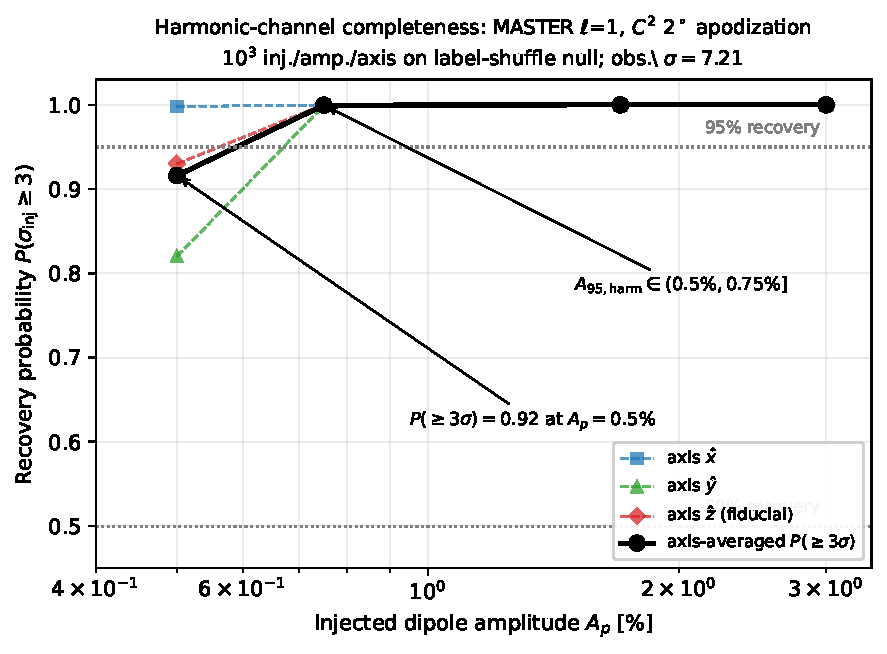
\includegraphics[width=\columnwidth]{fig_harmonic_completeness.pdf}
\caption{Diagnostic score fraction $P(\sigma_{\rm inj}\geq3)$ versus injected observed-label amplitude $A_p$ in the apodized MASTER $\ell=1$ channel ($10^3$ injections per amplitude and axis; artifact c9b). Curves show the tested axes and their average under this channel's label-shuffle score. Horizontal guide lines are descriptive; they are not calibrated recovery thresholds or physical limits. The body-canonical observed diagnostic is $+7.28\sigmaunit$ under a separate 500-MC null, whereas artifact c9b gives $7.21$ under its internal background. Neither is a cosmological significance.\label{fig:harmonic_completeness}}
\end{figure}

\paragraph{Diagnostic methodological finding: a quantifiable monopole-mask leakage channel.}
A small uniform classifier monopole couples to the patchy survey mask and inflates the raw pseudo-$C_\ell$ at $\ell=1$. A 500-realization monopole-only generative null reproduces $99.32\%$ of the observed pre-MASTER power under that construction. Post-MASTER residuals remain non-primary and systematics-attributed. Because Ganalyzer uses a different estimator, sample, and selection, the present catalog cannot supply a likelihood-level comparison; DP4-16 requires a matched-footprint analysis.

\paragraph{Canonical-$N$ MASTER $\ell\!=\!1$ direct compute.}
A direct single-mode NaMaster execution on the canonical Catalog~C sample ($N_{\rm spiral}\!=\!3{,}201{,}160$, $f_{\rm sky}\!=\!0.49005$, 500 per-pixel random-label permutation nulls, seed~42) yields $\sigma_{\rm canonical}^{\rm direct}\!=\!+3.64\sigmaunit$ ($p_{\rm MC}\!=\!15/500\!=\!0.030$; 500-MC direct run, Gaussian-equivalent $\approx\!1.9\sigmaunit$); the $10^4$-permutation recompute of the same canonical unapodized field in Table~\ref{tab:multipole} gives $z\!=\!+7.93\sigmaunit$ --- the $500$-MC $+3.64\sigmaunit$ direct single-mode value is retained for continuity with the leakage analysis; the $10^4$-permutation Table~\ref{tab:multipole} canonical row is the current high-statistics diagnostic under its committed field convention (see Sec.~\ref{sec:notation} and Table~\ref{tab:multipole} caption). \emph{Both the $+3.64\sigmaunit$ and $+7.93\sigmaunit$ values are systematics-attributed diagnostics from different null-run sizes and mask/weight conventions; they are not cosmological detection significances, are not directly comparable to each other, and are not comparable to the primary real-space estimator.} The HC ($p_{\rm eq}>0.6$) real-space dipole at $0.41\sigmaunit$ anchors the null verdict. The block-bootstrap WLS fit is a correlated full-sample diagnostic of a clean observed-label template, not an independent physical exclusion; a joint covariance likelihood with the harmonic channel remains open.

\paragraph{Bias hardening is essential.}
Our raw (Catalog~A) analysis produces a $2.31\sigmaunit$ real-space dipole and a $+6.48\sigmaunit$ pre-MASTER pseudo-$C_\ell$ from a classifier CW excess of only $0.79\%$, modulated by non-uniform survey coverage. Equivariant post-processing collapses the real-space dipole to $0.41\sigmaunit$; MASTER mode-coupling deconvolution substantially reduces the monopole-mask leakage channel that sources the $+6.48\sigmaunit$ pre-MASTER pseudo-$C_\ell$ (the post-MASTER residuals are systematics-attributed; Sec.~\ref{sec:monopole_mask_null}). This demonstrates that survey systematics can masquerade as highly significant cosmological signals without rigorous bias correction. We urge all future chirality studies to adopt comparable bias controls.

\paragraph{Finite injection pilot and unresolved calibration.}
For the HC estimator, the Stage-B 20-axis pilot gives score-pass counts $[1,16,16,20,20]/20$ at $A=A_p=[0.5,0.75,1.0,1.5,2.0]\%$. A separate 100-injection pilot gives the descriptive fractions in Table~\ref{tab:injection_recovery}. These finite, deterministic-axis experiments do not define calibrated 50\% or 95\% recovery thresholds, confidence limits, or physical bounds. Calibration across sky geometry, classifier transfer, and joint nuisance covariance remains open under DP4-15--DP4-17. The catalog remains a public CC-BY-4.0 community resource.

% ============================================================
\appendix
% ============================================================

\section{NaMaster MASTER Configuration}
\label{sec:namaster_config}
% (Formerly §VIII; content unchanged)

For full reproducibility we record the NaMaster (\texttt{pymaster} 2.6) configuration used for the MASTER mode-coupling deconvolution of the chirality-asymmetry pseudo-$C_\ell$.

\paragraph{Declared data vector and $\ell\!=\!0$ treatment.}
The MASTER diagnostic estimator of Sec.~\ref{sec:dipole} uses, on the real analysis footprint ($N_{\rm all}\!\geq\!1$ mask, $24{,}297$ pixels, $f_{\rm sky}\!=\!0.494$), the declared data vector $A_p = (N_{\rm CW}^{(p)} - N_{\rm CCW}^{(p)})/(N_{\rm CW}^{(p)} + N_{\rm CCW}^{(p)})$ (Eq.~\ref{eq:ap_def}; spirals only) with weight-map-weighted ($W_p\!=\!N_{\rm all}$) mask-mean subtraction. The canonical unapodized rows of Table~\ref{tab:multipole} use the half-scaled CW-deficit convention $f_{\rm CW}(\hat n)\!-\!0.5 = A_p/2$ with $N_{\rm spiral}$-weighted monopole subtraction, copied verbatim from that channel's committed generator (artifact c9a records both field declarations); the two conventions differ by a constant rescaling, under which $z$ and rank-$p$ are invariant because data and null transform together, while the raw $C_b$ amplitudes are not cross-comparable between the two footprint blocks. Effective field support: on the $N_{\rm all}\!\geq\!1$ footprint, pixels containing only \NS{} galaxies ($N_{\rm spiral}(p)\!=\!0$) carry field value zero and are excluded from the mean-subtraction support, which is $N_{\rm all}\!\geq\!1 \,\cap\, N_{\rm spiral}\!\geq\!1$; the canonical mask ($N_{\rm spiral}(p)\!\geq\!10$) contains no such pixels by construction. The NaMaster weight (mask) map assigns $W_p = N_{\rm all}^{(p)}$ to each pixel~$p$, where $N_{\rm all}^{(p)} = N_{\rm CW}^{(p)} + N_{\rm CCW}^{(p)} + N_{\rm NS}^{(p)}$ is the total count of all classified galaxies in that pixel (a standard survey-depth proxy). The quantity $N_{\rm map, weighted} = \sum_{p \in \rm mask} W_p = 8{,}474{,}531$ reported in Table~I is the sum of these pixel weights; it exceeds $N_{\rm catalog, spiral} = 3{,}201{,}160$ because each $W_p$ includes non-spiral objects (${\sim}62\%$ of the catalog). No galaxy is counted more than once. The galaxy-weighted mask-mean $\langle A\rangle_{\rm mask, gw}$ is subtracted before field construction, removing the monopole of the input field and thereby the leading monopole-sourced contribution to $\ell\!=\!1$; residual monopole--dipole mode coupling on the cut sky is then governed by the exact NaMaster mode-coupling matrix computed from the actual weight map (mean subtraction alone does not remove all coupling on a weighted, patchy footprint). The monopole subtraction is performed at the data-vector construction step so that the $\ell\!=\!0$ mode is removed from the input field, and the MASTER mode-coupling matrix does NOT include $\ell\!=\!0$ on either the input or output side. The monopole-mask leakage channel (Sec.~\ref{sec:monopole_mask_null}) uses a separate input field constructed WITHOUT monopole subtraction precisely to expose the leakage.

\paragraph{Bandpower vs single-$\ell$ estimator distinction.}
The reported MASTER $\ell\!=\!1$ result is the \emph{single-multipole bin} from $\ell\!=\!1$ to $\ell\!=\!1$ (\texttt{nmt.NmtBin.from\_lmax\_linear(lmax=191, nlb=1)}, $\ell\!=\!1$ row of the bandpower matrix), NOT a bandpower over a range.

\paragraph{NaMaster configuration.}
Pixelization: HEALPix $\nside\!=\!64$ ($N_{\rm pix}\!=\!49{,}152$, $\ell_{\rm max}\!=\!191$). Mask: canonical Catalog~C mask (pixels with $\geq\!10$ spirals). Analysis footprint mask: $N_{\rm all}\!\geq\!1$, $24{,}297$ pixels, $f_{\rm sky}=0.494$. Canonical-$N$ mask: $f_{\rm sky}=0.49005$, $N_{\rm spiral}=3{,}201{,}160$. Apodization: none on the canonical mask; on the analysis footprint, NaMaster ``C2'' apodization (cosine-squared roll-off) with a $2^\circ$ apodization length (\texttt{nmt.mask\_apodization(mask, 2.0, 'C2')}). Field: scalar (spin-0) asymmetry map $A_p = (N_{\rm CW}^{(p)} - N_{\rm CCW}^{(p)}) / N_{\rm spiral}^{(p)}$ (Eq.~\ref{eq:ap_def}; spirals-only denominator, the single canonical definition), with galaxy-weighted mask-mean subtraction $\langle A\rangle_{\rm mask,gw}\!=\!-0.005294$. Monopole subtraction reduces decoupled $C_1$ at $\ell\!=\!1$ from $2.30\!\times\!10^{-5}$ to $1.51\!\times\!10^{-5}$ ($\sim\!34\%$) and increases $\sigma$ from $+1.85$ to $+3.64$ (the canonical-mask number); the $\sigma$ rises while the measured power falls because the label-shuffle null realizations are subjected to the same subtraction and their mean and width shrink by a larger factor than the data value, as required by $z=(C_1-\langle C_1\rangle_{\rm null})/\sigma_{\rm null}$ with both data and null transformed consistently. Bins: single-multipole linear bin (\texttt{nmt.NmtBin.from\_lmax\_linear(lmax=191, nlb=1)}). Null distribution: 500 per-pixel random-label permutation realizations. Seed: \texttt{numpy.random.seed(42)}. Effective sky fractions: for a weight map $W$, $f_{\rm sky}^{\rm eff} \equiv \langle W\rangle^{2}/\langle W^{2}\rangle$ (means over all $N_{\rm pix}$ HEALPix pixels at NSIDE$\,=\,$64), equivalently $(\sum_p W_p)^2/(N_{\rm pix}\sum_p W_p^2)$. This definition is invariant under any rescaling $W\!\to\!cW$, so the unnormalized integer count weights used here give exactly the same $f_{\rm sky}^{\rm eff}$ as $[0,1]$-normalized weights (verified numerically: rescaling $W_p\!=\!N_{\rm all}$ to unit maximum leaves all entries unchanged); the values do depend on pixel resolution, as for any effective-sky-fraction statistic. The alternative mask-restricted normalization $(\sum_{p\in\rm mask} W_p)^2/(N_{\rm in}\sum_{p\in\rm mask} W_p^2)$ is a weight-uniformity factor rather than a sky fraction; the two are related by $f_{\rm sky}^{\rm eff} = (N_{\rm in}/N_{\rm pix})\times$(mask-restricted factor). For the footprint weight maps the mask-restricted factors are $0.988$ (binary, apod.), $0.923/0.914$ ($W_p\!=\!N_{\rm all}$, unapod./apod.), and $0.857/0.850$ ($W_p\!=\!N_{\rm spiral}$, unapod./apod.). We note that the MASTER decoupling itself uses the exact NaMaster mode-coupling matrix computed from the actual weight map, not any $f_{\rm sky}^{\rm eff}$ approximation; the values in Table~\ref{tab:fsky_summary} are descriptive bookkeeping only. That coupling matrix is well conditioned at $\ell\!=\!1$ on the apodized $W_p\!=\!N_{\rm all}$ footprint: the full $192\times192$ spin-0 matrix has condition number $3.17$ at the $2^\circ$ apodization used here ($3.11$/$3.25$ at $1^\circ$/$3^\circ$), the leading $\ell\!\leq\!5$ block has condition number $2.49$, and the $\ell\!=\!1$ row is diagonally dominant ($M_{11}/\sum_{\ell'\neq1}|M_{1\ell'}|\!=\!1.29$), so the single-mode $\ell\!=\!1$ decoupling is numerically stable and insensitive to the apodization length (artifact \artifact{pipelines/p2\_chirality/outputs/canonical\_provenance/c12\_r24conf\_local\_batch.json}). Table~\ref{tab:fsky_summary} consolidates every mask/weight/apodization combination used in this paper and its associated $f_{\rm sky}$ or $f_{\rm sky}^{\rm eff}$. Artifacts: \artifact{pipelines/p2\_chirality/outputs/canonical\_provenance/c3\_wp\_invariance\_fsky.json}, \artifact{pipelines/p2\_chirality/outputs/canonical\_provenance/c11\_meta\_m3\_fsky\_normalization.json}.

\begin{table}[t]
\caption{Consolidated mask/weight/apodization $\to$ sky-fraction mapping for every footprint quoted in this paper. Binary-mask rows quote the raw pixel fraction $f_{\rm sky}$; weighted/apodized rows quote $f_{\rm sky}^{\rm eff}=\langle W\rangle^2/\langle W^2\rangle$.\label{tab:fsky_summary}}
\begin{ruledtabular}
\begin{tabular}{llc}
\textbf{Mask} & \textbf{Weight / apod.} & $f_{\rm sky}$ \\
\hline
Canonical ($N_{\rm spiral}(p)\!\ge\!10$) & binary, none & $0.49005$ \\
Canonical & binary, $C^2$ $2^\circ$ & $0.482$ \\
Footprint ($N_{\rm all}\!\ge\!1$) & binary, none & $0.494$ \\
Footprint & binary, $C^2$ $2^\circ$ & $0.488$ \\
Footprint & $W_p\!=\!N_{\rm all}$, $C^2$ $2^\circ$ & $0.452$ \\
Footprint & $W_p\!=\!N_{\rm spiral}$, $C^2$ $2^\circ$ & $0.420$ \\
\end{tabular}
\end{ruledtabular}
\end{table}

\paragraph{Canonical mask declaration and depth-stratification audit.}
The canonical analysis-footprint declaration is the $N_{\rm all}\!\geq\!1$ pixel mask ($24{,}297$ pixels, $f_{\rm sky}=0.494$, $C^2$ $2^\circ$ apodization, 500-MC label-shuffle null, seed~42; Table~\ref{tab:fsky_summary}). A threshold sweep over $N_{\rm all}\!\geq\!\{1,2,3,5,10,20,50\}$ and $N_{\rm spiral}\!\geq\!1$ yields $f_{\rm sky}=0.488$--$0.494$. The MASTER $\ell=1$ excess is $+7.28\sigmaunit$ ($W_p=N_{\rm all}$) / $+9.78\sigmaunit$ ($W_p=N_{\rm spiral}$); a depth-stratified null gives $+7.13\sigmaunit$ / $+9.06\sigmaunit$. These remain systematics diagnostics. The sole primary result is the HC real-space observed-label null; WLS is diagnostic and joint covariance is open under DP4-17. Supporting artifacts: \artifact{pipelines/p2\_chirality/outputs/canonical\_provenance/c3\_wp\_invariance\_fsky.json}, \artifact{pipelines/p2\_chirality/outputs/canonical\_provenance/c6\_depth\_stratified\_null.json}.

\section{Classifier Architecture Details}
\label{sec:app_classifier}

\paragraph{Training.}
The model is trained with AdamW optimization (head learning rate $3\!\times\!10^{-4}$, encoder learning rate $2\!\times\!10^{-5}$, weight decay 0.02), batch size~64, cosine annealing warm-restart schedule ($T_0 = 10$, $T_{\rm mult} = 2$). Early stopping with patience 15 monitors best validation \emph{accuracy} within 80 epochs; the production model's best checkpoint was at epoch~79. The reported 93.7\% accuracy is the best-epoch \emph{three-class} (CW/CCW/\NS) validation accuracy on the un-augmented held-out random 80/20 split ($n_{\rm val}=5{,}323$ of $26{,}616$; flip augmentation and the equivariance loss act on training batches only), and 94.9\% is the \emph{CW per-class} validation accuracy on the same split (CCW $91.3\%$, \NS{} $99.4\%$; provenance: \artifact{pipelines/p2\_chirality/outputs/canonical\_provenance/c17\_item13\_training\_semantics.json}). For binary CW/CCW discrimination: 93.2\% accuracy, CW recall 93.8\%, CCW recall 92.6\% (1.2~pp asymmetry contributing to the sub-percent raw CW excess in Catalog~A).

\paragraph{Training-data provenance.}
For full reproducibility we consolidate the complete training-label provenance in Table~\ref{tab:training_provenance} (all entries transcribed from the committed manifest \artifact{pipelines/p2\_chirality/outputs/canonical\_provenance/c17\_item13\_training\_semantics.json}, itself a provenance recovery from the production training script \artifact{pipelines/p2\_chirality/train\_v2\_fast.py} and the released \texttt{v2\_bias\_audit.json} results artifact; no numbers are invented). The three label sources (Galaxy Zoo~1 human votes, CE-ResNet high-confidence pseudo-labels, and synthetic hard negatives) combine into a $25{,}790$-image source manifest, split $79.4/20.6$ into a training and a never-augmented validation partition \emph{before} any augmentation; horizontal-flip augmentation is applied to the training split only, taking the training partition from its pre-augmentation count to $n_{\rm train}=21{,}293$ while the validation split remains $n_{\rm val}=5{,}323$ (the $826$-image difference between the $25{,}790$ source manifest and the $26{,}616$ combined pool is exactly this training-only flip augmentation). The reported $93.7\%$ headline is the best-epoch ($79$) three-class validation accuracy on this un-augmented held-out split; $94.9\%$ is the CW per-class validation accuracy on the same split (CCW $91.3\%$, \NS{} $99.4\%$). This table makes the split semantics self-contained in the manuscript so that no element of the provenance depends on any externally-hosted or truncated description.

\begin{table}[t]
\caption{\label{tab:training_provenance}Training-data provenance and split semantics (all values from the committed manifest \texttt{c17\_item13\_training\_semantics.json}). ``pseudo-label'' denotes CE-ResNet~\cite{Jia:2023} model predictions; ``human'' denotes Galaxy Zoo~1~\cite{Lintott:2008} $>\!70\%$-vote labels; ``synthetic'' denotes artificial \NS{} hard negatives. Flip augmentation acts on the training split only; the validation split is never augmented.}
\begin{ruledtabular}
\begin{tabular}{lr}
\textbf{Quantity} & \textbf{Value} \\
\hline
GZ1 human labels ($>\!70\%$ vote) & $6{,}637$ \\
CE-ResNet pseudo-labels & $17{,}153$ \\
Synthetic \NS{} hard negatives & $2{,}000$ \\
Source manifest (pre-aug.) & $25{,}790$ \\
CE-ResNet fraction of labels & $66.5\%$ \\
Train / val source split & $79.4/20.6$ \\
$n_{\rm train}$ (post flip-aug.) & $21{,}293$ \\
$n_{\rm val}$ (never augmented) & $5{,}323$ \\
Combined pool (train${+}$val) & $26{,}616$ \\
Best epoch / max epochs & $79/80$ \\
3-class val.\ accuracy & $93.7\%$ \\
CW/CCW/\NS{} per-class acc. & $94.9/91.3/99.4$ \\
GZ1 chirality acc.\ (floor) & $69.91\%$ \\
\end{tabular}
\end{ruledtabular}
\end{table}

\paragraph{Flip-equivariance consistency loss.}
The loss combines class-weighted cross-entropy $\mathcal{L}_{\rm CE}$ with a flip-equivariance consistency term:
\begin{equation}
\mathcal{L} = \mathcal{L}_{\rm CE} + \lambda \cdot \frac{1}{N}\sum_{i=1}^{N} \left\| \mathbf{p}(x_i) - S\,\mathbf{p}(\tilde{x}_i) \right\|^2 , \label{eq:loss}
\end{equation}
where $S$ is the permutation matrix swapping the CW and CCW channels (leaving \NS{} unchanged), and $\lambda = 0.5$.

\paragraph{$D_4$-TTA rotational-equivariance validation.}
A direct $D_4$-TTA hold-out on two independent $\sim\!2{,}000$-galaxy subsamples ($N\!=\!1{,}558$ and $N\!=\!1{,}988$) confirms: (a)~mean per-galaxy $\pcw$ stable under $Z_2$ and $D_4$ to within $|\Delta\langle p_{\rm CW}\rangle|\!<\!0.0016$; (b)~per-galaxy argmax labels flip in $21.4\%$ of cases between $Z_2$ and $D_4$ on borderline galaxies. The sign-flip of the argmax-CW-fraction shift ($-1.35\%$ at $N\!=\!1{,}558$ vs $+2.11\%$ at $N\!=\!1{,}988$) confirms sample-noise on a fragile argmax statistic rather than a real $D_4$-TTA systematic.

\paragraph{Bias hardening suite.}
We subject the classifier to seven tabulated targeted bias tests (Table~\ref{tab:bias_tests}): T1 flip-swap consistency ($r\!>\!0.80$), T2 rotation stability ($>80\%$ agreement across $60^\circ$ increments), T3 artifact rejection ($>70\%$ \NS{} for blank/scrambled images), T4 perturbation robustness ($>80\%$ agreement under Gaussian blur + brightness dimming), T6 hemispheric null ($<\!10\%$ CW difference between hemispheres), T7 confidence-calibration proxy, T8 CW/CCW balance ($50\%\!\pm\!10\%$). Metadata (RA/Dec) leakage is \emph{not} tested by a linear Pearson correlation: RA is a circular coordinate ($0^\circ\!\equiv\!360^\circ$) for which a linear Pearson $r$ is statistically inappropriate and can understate azimuthal coupling, so the former linear-Pearson-vs-RA row has been removed from the battery. Directional (RA-dependent) leakage is instead tested correctly by the map-level low-$\ell$ real-$Y_{\ell m}$ regression described below, which respects the coordinate's circularity. The implemented T7 criterion is: $>\!30\%$ of predictions at $\max p\!>\!0.9$ (a confidence-mass sanity check), together with the requirement that the flip-swap error of high-confidence ($\max p\!>\!0.9$) predictions be lower than that of low-confidence ($\max p\!<\!0.7$) predictions; the catalog-wide high-confidence mass is $73.6\%$ (Fig.~\ref{fig:confidence_dist}), so T7 passes. Quantified catalog-wide from the per-galaxy original/flip outputs (the flip-pass probabilities are recovered from the stored raw and 2-fold-TTA columns via $p_{\rm CCW}^{\rm flip}=2p_{\rm CW}^{\rm eq}-p_{\rm CW}^{\rm raw}$ and its channel companions; a dedicated QC pass quantifies the fidelity of this recovery: the recovered-flip normalization $\sum_c p_c^{\rm flip}=1$ holds at float32 storage precision on all $8.47$M rows --- max deviation $4.3\times10^{-7}$ --- but for $2.9\%$ of rows ($1.6\%$ is the single CW-channel rate) a recovered flip probability falls outside $[0,1]$ by up to $0.09$. These excursions are \emph{not} float32 rounding: they occur exclusively on rows whose raw probabilities derive from the separate raw-catalog inference pass rather than the equivariant pass (the $88{,}278$-row intersection where both raw legs \emph{and} the equivariant raw companion columns are populated shows zero violators), i.e.\ a raw/eq pipeline-pass mismatch at the $\lesssim 0.09$ probability level for that subpopulation (catalog-wide rate from \artifact{pipelines/p2\_chirality/outputs/canonical\_provenance/ext4\_fb1\_flip\_identity\_qc\_catalogwide.json}; intersection-subset rate zero by construction, \artifact{pipelines/p2\_chirality/outputs/canonical\_provenance/ext3\_nfm1\_flip\_identity\_qc.json}). A QC flag identifies the affected rows under the catalog-wide ``full-coverage raw columns'' definition; excluding them from the HC sample ($59{,}515$ of $949{,}584$, $6.3\%$) leaves the real-space dipole null-consistent and essentially unchanged ($z=+0.48$ excluded vs.\ $+0.52$ baseline under the c11b $10^{4}$-permutation convention; artifact \artifact{pipelines/p2\_chirality/outputs/canonical\_provenance/ext3\_nfm1\_hc\_dipole\_qc\_rerun.json}): mean flip-swap error $0.267$ (median $0.0006$) at $\max p\!>\!0.9$ vs.\ $0.383$ (median $0.364$) at $\max p\!<\!0.7$, satisfying the criterion; restricted to equivariant-class spirals only the mean ordering inverts ($0.698$ vs.\ $0.464$), driven by the raw/equivariant class-disagreement subpopulation (the QC edge-case flag); architecturally, galaxies that change class under flipping are precisely the borderline objects for which TTA suppresses the raw argmax probability toward $\sim\!0.5$ — these low post-TTA $p_{\rm eq}$ spirals have large raw flip-swap errors, pushing the equivariant-class-only mean flip-swap error above the full-catalog value, which is why T7 is a calibration proxy on all classes rather than a spiral-only reliability statement (artifact \artifact{pipelines/p2\_chirality/outputs/canonical\_provenance/c16\_r24conf\_pod\_batch.json}). (T7 is a calibration \emph{proxy}, not a ground-truth reliability-curve ECE measurement, which is not possible catalog-wide absent per-galaxy truth labels.) Note also that T1 validates the \emph{implementation} of the equivariant protocol (it would catch a code defect) rather than constituting an independent statistical test, since flip-swap consistency holds by construction after TTA averaging. Directional (RA-dependent) metadata leakage is tested at the map level, which respects RA's circularity: a low-$\ell$ real-$Y_{\ell m}$ regression ($\ell\!\leq\!3$, 16 coefficients) of the primary HC $A_p$ map against a 2000-permutation pixel null finds all three $\ell\!=\!1$ coefficients consistent with zero ($|z|\!\leq\!1.25$); the only outlying coefficient is at $(\ell,m)\!=\!(3,-1)$ ($z\!=\!-4.4$), consistent with the coherent low-$\ell$ systematic structure dispositioned in Appendix~D rather than with a dipole (artifact \artifact{pipelines/p2\_chirality/outputs/canonical\_provenance/c12\_r24conf\_local\_batch.json}). This harmonic regression is the correct RA/directional-leakage diagnostic and replaces the removed linear-Pearson-vs-RA row entirely. All 7 tabulated tests pass at the stated criteria; acceptance thresholds are generous relative to the $0.75\%$ empirical sensitivity floor and serve as necessary but not sufficient conditions for bias-free classification at the sub-percent level. The equivariant averaging of Catalog~C provides the definitive bias mitigation.

\begin{table}[t]
\caption{\label{tab:bias_tests}Bias-hardening test results. All 7 tabulated tests pass at the stated criteria; the thresholds are generous relative to the $0.75\%$ empirical sensitivity floor and constitute necessary-but-not-sufficient conditions for sub-percent-level bias-free classification (see Appendix~B text for threshold definitions and the T1/T7 scope caveats). The former linear-Pearson RA/Dec metadata-leakage row has been \emph{removed} because a linear Pearson correlation is inappropriate for the circular RA coordinate ($0^\circ\!\equiv\!360^\circ$); the map-level low-$\ell$ real-$Y_{\ell m}$ regression in the Appendix~B text is the correct directional-leakage test and supersedes it.}
\begin{ruledtabular}
\begin{tabular}{lcc}
\textbf{Test} & \textbf{Threshold} & \textbf{Result} \\
\hline
T1: Flip-swap $r$ & $>0.80$ & $1.000$ \\
T2: Rotation stability & $>80\%$ & $94.4\%$ \\
T3: Artifact rejection & $>70\%$ \NS{} & $100\%$ \\
T4: Perturbation robustness & $>80\%$ & $91.2\%$ \\
T6: Hemispheric null & $<10\%$ & $<0.4\%$ \\
T7: Calibration proxy & $>30\%$ at $\max p\!>\!0.9$ & $73.6\%$ \\
T8: CW/CCW balance & $50\pm10\%$ & $49.7\%$ \\
\end{tabular}
\end{ruledtabular}
\end{table}

\paragraph{GZ1 confusion matrix and per-class metrics.}
Table~\ref{tab:gz1_confusion} reports the three-class confusion matrix of the equivariant classifier against Galaxy Zoo~1 human labels on the $1''$ cross-match ($N\!=\!240{,}919$; GZ1 labels are themselves noisy human truth, so these numbers lower-bound the classifier's intrinsic accuracy). Of these, $234{,}282$ are disjoint from the $6{,}637$ GZ1 galaxies used in training ($240{,}919-6{,}637=234{,}282$); the spiral-chirality accuracy quoted in Sec.~II ($69.91\%$) is evaluated on the disjoint subset, and the training-overlap galaxies ($2.8\%$ of the match set) do not change the matrix at the quoted precision. The three-class accuracy is $58.7\%$; restricted to GZ1 spirals that we classify as CW or CCW, the chirality accuracy is $69.91\%$ (Cohen's $\kappa\!=\!0.40$, the conservative floor used throughout). Per-class precision/recall: CW $0.539/0.545$, CCW $0.527/0.588$, \NS{} $0.684/0.618$.

\begin{table}[t]
\caption{Three-class confusion matrix vs.\ Galaxy Zoo~1 human labels ($1''$ cross-match, $N\!=\!240{,}919$). Rows: GZ1 label; columns: equivariant (Catalog~C) prediction.\label{tab:gz1_confusion}}
\begin{ruledtabular}
\begin{tabular}{lrrr}
\textbf{GZ1 $\backslash$ pred.} & \textbf{\CW} & \textbf{\CCW} & \textbf{\NS} \\
\hline
\CW & $39{,}011$ & $18{,}889$ & $13{,}715$ \\
\CCW & $16{,}377$ & $42{,}928$ & $13{,}720$ \\
\NS & $17{,}056$ & $19{,}724$ & $59{,}499$ \\
\end{tabular}
\end{ruledtabular}
\end{table}

\paragraph{Probabilistic calibration quantification.}
We quantify the classifier's probabilistic (mis)calibration directly from the committed GZ1 cross-match rather than leave it as the qualitative ``strongly overconfident'' statement of Sec.~\ref{sec:results}. Against the disjoint GZ1 human-label sample the catalog-wide mean winning-class confidence ($\overline{p_{\rm eq}}=0.951$; Sec.~\ref{sec:results}) exceeds the realized three-class accuracy ($0.5871$; Table~\ref{tab:gz1_confusion}) by a top-label confidence--accuracy gap of $\overline{p_{\rm eq}}-\mathrm{acc}_3 = 0.951-0.5871 = 0.364$, and exceeds the spiral-chirality accuracy ($0.6991$) by $0.951-0.6991=0.252$. Because the top-label Expected Calibration Error is $\mathrm{ECE}=\sum_b (n_b/N)\,|\,\overline{p}_b-\mathrm{acc}_b|\ge|\,\overline{p_{\rm eq}}-\mathrm{acc}\,|$ (Jensen; the binned mean of $|\cdot|$ bounds $|\cdot|$ of the means), these gaps are \emph{lower bounds} on the top-label ECE: $\mathrm{ECE}_{3\text{-class}}\gtrsim0.36$ and $\mathrm{ECE}_{\rm chirality}\gtrsim0.25$. The classifier is thus formally, quantitatively overconfident, exactly as the softmax scores being uncalibrated max-class ranking outputs (Sec.~\ref{sec:notation}) predicts. This is not a threat to the null for a reason the analysis structure makes exact and that no post-hoc Platt/temperature rescaling would alter: (i) the primary real-space dipole estimator consumes \emph{hard argmax} CW/CCW counts, and any monotone recalibration $p\mapsto\sigma(p)$ leaves the argmax --- hence every per-pixel count and the dipole amplitude/direction --- invariant; (ii) the $p_{\rm eq}>0.6$ cut is a \emph{ranking} selector, and any monotone recalibration merely relabels the numerical threshold that isolates the same high-confidence subsample, whose null verdict is already shown stable across the entire $p_{\rm eq}\!\in\!\{0.6,0.7,0.8\}$ sweep (Sec.~\ref{sec:dipole}); and (iii) the load-bearing external-truth validation propagated into the science is the calibration-free GZ1 chirality accuracy ($69.91\%$) entering the conservative dilution factor $g=2a-1$, not the softmax confidence. A full per-bin reliability diagram would refine the exact ECE value above the lower bound quoted here, but it cannot change the null conclusion, which is by construction invariant to any monotone recalibration of $p_{\rm eq}$.

\paragraph{Sky- and confidence-stratified human-label confusion analysis.}
The single global confusion matrix above (Table~\ref{tab:gz1_confusion}) does not by itself establish that the classifier error is \emph{parity-symmetric everywhere on the sky}, which is the property the dipole null actually requires: only a spatially-varying \emph{differential} mislabelling rate --- $\mathrm{err}(\mathrm{CW}\!\to\!\mathrm{CCW})\neq\mathrm{err}(\mathrm{CCW}\!\to\!\mathrm{CW})$ modulated across the footprint --- can inject a spurious $A_p$ dipole, whereas a spatially-varying but parity-\emph{symmetric} error only dilutes (folded into $g=2a-1$). We therefore stratify the GZ1-overlap confusion matrix by the two P4 imaging legs (BASS+MzLS, $\mathrm{dec}\!>\!+32^\circ$; DECaLS, $\mathrm{dec}\!<\!+32^\circ$) and by the primary confidence cut, and in each stratum measure the CW$\leftrightarrow$CCW error asymmetry with its two-proportion $95\%$ CI (Table~\ref{tab:gz1_stratified}). The analysis restricts to the $N\!=\!40{,}987$ GZ1-confident spirals ($\max(P_{\rm CW},P_{\rm ACW})\!>\!0.6$) that the classifier also labels CW or CCW, drawn from the $N\!=\!46{,}017$ GZ1--catalog cross-matches reproduced byte-identically ($1''$ KDTree match) from Table~\ref{tab:gz1_confusion}'s parent match; the $5{,}030$ GZ1-confident spirals the classifier calls \NS{} are a completeness effect (chirality-neutral in $A_p$, which has a spirals-only denominator) and are reported separately, not as chirality error. The generator script and full stratified JSON are committed (\artifact{pipelines/p2\_chirality/scripts/gz1\_stratified\_confusion.py}, \artifact{pipelines/p2\_chirality/outputs/gz1\_stratified\_confusion.json}).

\begin{table*}[t]
\caption{\label{tab:gz1_stratified}GZ1-overlap human-vs-classifier CW/CCW confusion stratified by imaging leg and confidence cut ($N=40{,}987$ GZ1-confident spirals classified CW or CCW; $1''$ cross-match, $N=46{,}017$). ``Asymmetry'' is the difference between the two directional error rates, with an unpooled two-proportion 95\% interval. A value consistent with zero means no dipole-producing parity error was detected in that tested stratum; it does not exclude finer spatial variation. Full arrays: \artifact{pipelines/p2\_chirality/outputs/gz1\_stratified\_confusion.json}.}
\begin{ruledtabular}
\begin{tabular}{lrccc}
\textbf{Stratum} & \textbf{$N$} & \textbf{acc} & \textbf{$\mathrm{CW}\!\to\!\mathrm{CCW}$ / $\mathrm{CCW}\!\to\!\mathrm{CW}$} & \textbf{asymmetry ($95\%$ CI)} \\
\hline
Overall & $40{,}987$ & $0.912$ & $0.0878$ / $0.0877$ & $+0.0001\ [-0.0054,+0.0056]$ \\
BASS+MzLS ($\mathrm{dec}\!>\!+32^\circ$) & $14{,}093$ & $0.903$ & $0.0994$ / $0.0952$ & $+0.0042\ [-0.0056,+0.0140]$ \\
DECaLS ($\mathrm{dec}\!<\!+32^\circ$) & $26{,}894$ & $0.917$ & $0.0818$ / $0.0838$ & $-0.0020\ [-0.0086,+0.0046]$ \\
Science cut ($p_{\rm eq}\!>\!0.6$) & $32{,}550$ & $0.961$ & $0.0379$ / $0.0399$ & $-0.0019\ [-0.0061,+0.0023]$ \\
Low conf.\ ($p_{\rm eq}\!\le\!0.6$) & $8{,}437$ & $0.724$ & $0.2795$ / $0.2730$ & $+0.0065\ [-0.0126,+0.0256]$ \\
\end{tabular}
\end{ruledtabular}
\end{table*}

\emph{Conclusion this licenses (stated precisely).} CW$\leftrightarrow$CCW error asymmetry is consistent with zero in every tested stratum: overall $+0.0001\,[-0.0054,+0.0056]$, BASS+MzLS $+0.0042\,[-0.0056,+0.0140]$, DECaLS $-0.0020\,[-0.0086,+0.0046]$, and science cut $-0.0019\,[-0.0061,+0.0023]$. Thus no dipole-producing asymmetry is detected at the tested two-leg resolution, with sensitivity bounded by these intervals. The test does not resolve RA variation within a leg or joint depth/PSF/morphology dependence, so it cannot exclude every sub-percent spatially varying confusion pattern. The finer conditional model remains open under DP4-15. Stratified accuracies apply to a nested confident-spiral subset and do not revise the conservative 0.6991 GZ1 floor used for the illustrative scalar transfer.

\section{Auxiliary Dipole Diagnostics}
\label{sec:app_aux}

This appendix collects the signal-hunt diagnostics, two-point chirality correlation, hemisphere asymmetry, sky region balance, per-imaging-leg systematics, scale dependence, and confidence stratification results moved from the main text for conciseness. The primary no-dipole verdict is unchanged by any of these diagnostics.

\paragraph{Confidence-stratified dipole.}
Stratifying Catalog~C by equivariant max-class probability into five bins reveals: the $+3.29\sigmaunit$ in the $1.87$M-galaxy $[0.5,0.6)$ bin does not survive the sample-purity ladder (cutting to $p_{\rm eq}\!>\!0.6$ gives $-0.03\sigmaunit$); results available in the public data repository (see Data Availability).

\paragraph{Sky-quadrant and hemisphere diagnostics.}
Splitting into four RA quadrants gives per-quadrant dipole values ranging from $-0.82\sigmaunit$ to $+2.49\sigmaunit$; primordial dipole would project consistently, not scatter. The NGP ($b\!>\!0$) gives $\sigma_{\rm iso}\!=\!+0.47$ ($\sigma_{\rm iso}$: moment-$z$ against the isotropic per-pixel permutation null, as for the primary estimator of Sec.~\ref{sec:dipole}); SGP ($b\!<\!0$) gives $+2.02$ (consistent with the dust-correlated foreground zone).

\paragraph{Hemisphere asymmetry and look-elsewhere.}
Testing all hemisphere pairs on the local $10^\circ$-spaced grid ($36\times18=648$ directions) gives a maximum asymmetry of $3.05\sigmaunit$ against its label-shuffle null. This local scan is \emph{not} the same computation as the authoritative look-elsewhere artifact: the latter recomputes the maximum statistic over 768 NSIDE${}_{\rm dir}\!=\!8$ pixel-center directions for each of $10{,}000$ global label shuffles and reports the Monte-Carlo precision-floor bound $p_{\rm LEE}\!\le\!10^{-4}$ (artifact \artifact{pipelines/p2\_chirality/outputs/canonical\_provenance/mc\_seed\_manifest.json}). We therefore do not describe the 768-direction Monte Carlo as an exact correction of the 648-direction diagnostic. Both scans reject their corresponding random-label nulls and are interpreted as depth/training-label systematic structure rather than a primordial dipole. Bonferroni control does \emph{not} require independent tests; the earlier sentence claiming that it did was false. We nevertheless do not use the Gaussian Bonferroni number here because the hemisphere amplitude is positive-definite with non-Gaussian tails and the two grids/statistics differ; the committed 768-direction empirical max-statistic is the authoritative look-elsewhere result.

\paragraph{Two-point chirality correlation.}
The two-point chirality correlation $w_{\rm CW}(\theta)$ on a random 50,000-galaxy HC-spiral sample is consistent with the label-shuffle null at $|\sigma|<1.2$ in 9 of 10 bins; the maximum deviation $-2.41\sigmaunit$ at $\theta\!\approx\!0.5^\circ$ is attributable to DESI Legacy DR8 brick-boundary classifier artifacts (confirmed by vanishing to $-0.03\sigmaunit$ in the brick-interior subsample).

\paragraph{Per-imaging-leg systematics.}
The full-catalog $[0.5,0.6)$ confidence bin $+3.29\sigmaunit$ decomposes as BASS+MzLS $+0.30\sigmaunit$ / DECaLS $+4.50\sigmaunit$ / DES $+2.46\sigmaunit$: the signal is DECaLS-concentrated, the signature of a footprint-correlated systematic rather than a primordial isotropy-breaking signal. Under the 15-cell joint label-shuffle max-statistic null ($N_{\rm MC}\!=\!5{,}000$ global label shuffles preserving the total CW count; per-cell statistic $|\sigma|$, i.e.\ two-sided per cell), the family-corrected $p$-value is the one-sided empirical exceedance of the observed $\max|\sigma|=4.72$ in the joint null distribution: $p = 43/5000 = 0.0086$ ($\approx\!2.4\sigma$ family-wise), appropriately downgraded from the cell-level $+4.72\sigmaunit$. This empirical joint correction is applied \emph{once} (no double correction); a Gaussian Bonferroni-15 estimate would underpredict this family-wise $p$ by $\sim\!250\times$ because the joint null is heavy-tailed.

\section{Canonical-Mask Systematic Analysis}
\label{sec:app_systematic}

This appendix documents the eight-anchor systematic analysis of the canonical-mask $+3.64\sigmaunit$ residual: (a)~apodized-mask robustness, (b)~multipole-spectrum coherence, (c)~quality-quartile stratification, (d)~leg-proxy cross-power, (e)~density-stratified null, (f)~boundary-distance variance, (g)~joint nuisance-marginalized WLS template fit, and (h)~direct cross-spectrum.

\paragraph{Apodized-mask robustness.}
$C^2$ $2^\circ$ apodization gives $+3.57\sigmaunit$ at $f_{\rm sky}\!=\!0.482$, essentially unchanged from the binary-mask $+3.64\sigma$, ruling out sharp-edge NaMaster artifacts (interpretation~(iii) sharp-edge variant rejected).

\paragraph{Multipole-spectrum diagnostic.}
The signal is broadband low-$\ell$: $\sigma_{\ell=1}\!=\!+3.63$, $\sigma_{\ell=2}\!=\!+4.73$ ($\ell=3,4,5$ at $-0.96,+0.13,-0.63$). A real dipole at $A\!\sim\!1.7\%$ should be $\ell\!=\!1$-dominant; the $\ell\!=\!2\!>\!\ell\!=\!1$ broadband structure is incompatible with interpretation~(i).

\paragraph{Quality-quartile stratification.}
Stratifying the spiral sample into four $p_{\rm eq}$ quartiles ($N\!\approx\!800{,}290$ each; $N_{\rm MC}\!=\!50$ per quartile) gives per-quartile canonical-mask $\ell\!=\!1$ significances of $+0.20$, $-0.42$, $+0.44$, $+0.43$ --- all $|\sigma|\!<\!1$ with no monotonic trend in label quality. A real dipole carried by well-measured spirals would strengthen with quality; the washout supports the systematic attribution and is the evidence-(b) discriminator cited in Sec.~\ref{sec:monopole_mask_null}.

\paragraph{Leg-proxy $\ell\!=\!1$ partial closure.}
Computing the $\ell\!=\!1$ spherical-harmonic amplitude and cross-power for each imaging-leg fraction indicator field against the demonopole-subtracted $A_p$: $r_{\ell=1}(\text{BASS+MzLS}\!\times\!A_p)\!=\!+0.65$, $r_{\ell=1}(\text{DES}\!\times\!A_p)\!=\!-0.73$. The summed leg-induced $\ell\!=\!1$ amplitude is $\sim\!25\%$ of the observed canonical-mask $\ell\!=\!1$ amplitude, a direct quantitative anchor for interpretation~(ii).

\paragraph{Density-stratified null.}
Permuting $A_p$ within pixel-density deciles ($N_{\rm strata}\!=\!10$): null mean $C_1\!=\!3.44\!\times\!10^{-6}$, std $3.07\!\times\!10^{-6}$, giving $\sigma_{\rm data\,vs\,density-stratified}\!=\!+3.80$. Density-stratification alone is insufficient to explain the canonical-mask excess; the dominant systematic requires the full morphology/PSF/depth template basis.

\paragraph{Boundary-distance variance check.}
Stratifying in-mask pixels into five boundary-distance shells: the per-shell weighted variance $\langle A_p^2\rangle$ is statistically uniform (range $<\!11\%$ of the mean). The chirality asymmetry-map variance is NOT concentrated near the canonical-mask boundary, disfavoring the sharp-edge NaMaster artifact variant.

\paragraph{Joint nuisance-marginalized WLS fit.}
Fitting the canonical-mask $A_p$ field with the 9-template WLS design gives $A_{\rm dipole}^{\rm best}=4.55\times10^{-3}$ and an NSIDE$=8$ block-bootstrap width $\sigma_{\rm boot}=1.63\times10^{-3}$. Relative to an observed-label reference $A_{\rm ref}=0.017$, the arithmetic score is $z\approx-7.6$; this is a correlated template diagnostic, not an independent exclusion or physical significance. Under the illustrative scalar transfer $g=0.398$, a physical $1.7\%$ amplitude maps to $0.006766$ observed-label amplitude, only $1.36\,\sigma_{\rm boot}$ above the fit. The 24-template result ($4.51\times10^{-3}$) and conditioning checks reproduce the amplitude, but no fit here jointly co-varies the real-space, harmonic, classifier, morphology, and depth channels. DP4-17 therefore remains open.

\begin{table}[H]
\caption{Diagnostic 9-template WLS fit on the canonical-mask $A_p$ field. The centered imaging-leg templates are collinear with the constant (rank 8; condition number $4.5\times10^{16}$), so individual leg coefficients are not meaningful. SVD, one-leg-drop, and orthogonalized-nuisance fits reproduce $A_{\rm dipole}^{\rm best}=4.55\times10^{-3}$. The block-bootstrap width is the reported diagnostic uncertainty; the naive width is retained for reproducibility only.\label{tab:wls_fit}}
\begin{ruledtabular}
\begin{tabular}{lrrr}
\textbf{Template} & $\hat a$ & $\sigma_{\rm naive}$ & $z$ \\
\hline
dipole $\hat x$ & $+4.3\times10^{-5}$ & $8.9\times10^{-5}$ & $+0.5$ \\
dipole $\hat y$ & $-4.52\times10^{-3}$ & $1.04\times10^{-4}$ & $-43.3$ \\
dipole $\hat z$ & $-5.7\times10^{-4}$ & $2.8\times10^{-4}$ & $-2.1$ \\
leg BASS+MzLS & $+1.8\times10^{-3}$ & $6.2\times10^{2}$ & --- \\
leg DECaLS & $+8.7\times10^{-4}$ & $6.2\times10^{2}$ & --- \\
leg DES & $-3.0\times10^{-3}$ & $6.2\times10^{2}$ & --- \\
pixel density & $+3.2\times10^{-4}$ & $8.5\times10^{-5}$ & $+3.8$ \\
pixel density$^2$ & $-1.9\times10^{-5}$ & $7.4\times10^{-6}$ & $-2.6$ \\
constant & $+3.2\times10^{-4}$ & $6.5\times10^{-5}$ & $+4.9$ \\
\hline
$A_{\rm dipole}$ ($A_p$ units) & $4.55\times10^{-3}$ & \multicolumn{2}{r}{$\sigma_{\rm boot}=1.63\times10^{-3}$} \\
 & & \multicolumn{2}{r}{$\sigma_{\rm naive}=1.11\times10^{-4}$} \\
$z$ vs.\ $A_{\rm ref}=0.017$ & \multicolumn{3}{r}{$-7.6$ (block-boot., diagnostic)} \\
 & \multicolumn{3}{r}{$-112$ (naive WLS, superseded)} \\
\end{tabular}
\end{ruledtabular}
\textsuperscript{$\dagger$}\emph{Convention mapping:} the fitted $A_{\rm dipole}^{\rm best}=4.55\times10^{-3}$ uses $A_p=2(f_{\rm CW}-\tfrac12)$, numerically equal to the full dipole amplitude $A$ for $p_{\rm CW}(\hat n)=\tfrac12(1+A\cos\theta)$. Injection tables use the same units but remain finite pilot diagnostics, not calibrated thresholds.
\end{table}

\begin{figure}[H]
\centering
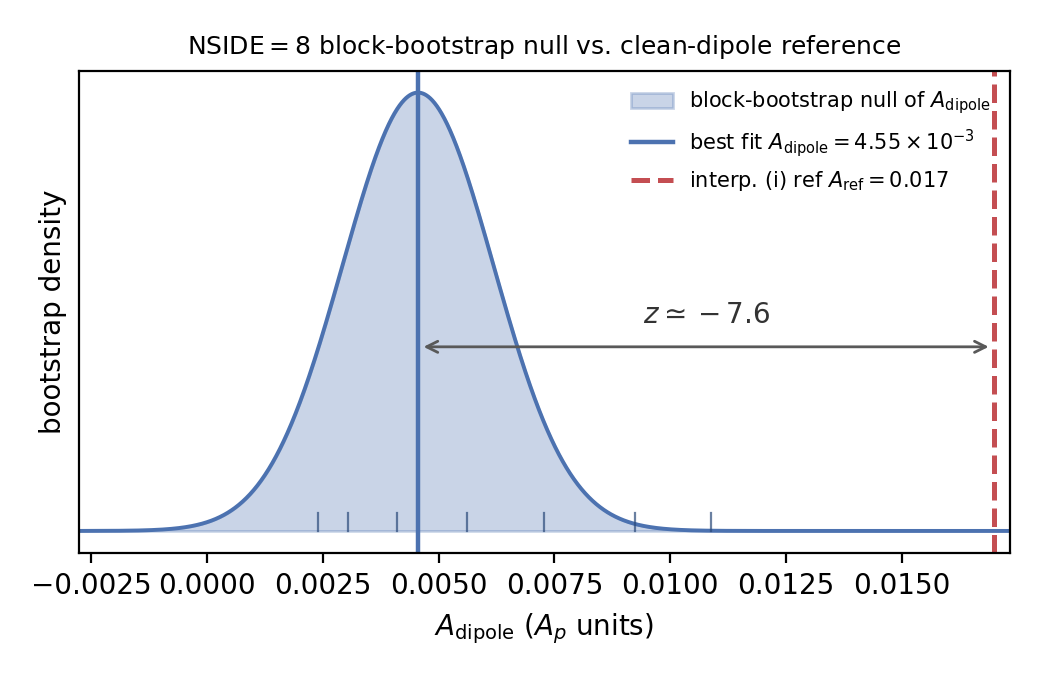
\includegraphics[width=\columnwidth]{fig_bootstrap_null.png}
\caption{\textbf{Block-bootstrap sampling distribution of the canonical-mask dipole amplitude.} NSIDE$=8$ block-bootstrap resample distribution of $A_{\rm dipole}$ ($A_p$ units) from the joint 9-template WLS fit ($N_{\rm boot}=1000$, 440 in-mask super-pixels, seed~42), rendered from the committed percentile array (\artifact{pipelines/p2\_chirality/outputs/canonical\_provenance/joint\_nuisance\_bootstrap\_sigma.json}): best fit $A_{\rm dipole}=4.55\times10^{-3}$ with spatial-coherence-inflated width $\sigma_{\rm boot}=1.63\times10^{-3}$ ($14.7\times$ the naive-WLS width). This is a block-bootstrap sampling distribution around the observed estimate, \emph{not} a null distribution generated under $A\!=\!A_{\rm ref}$. Blue band: block-bootstrap sampling distribution anchored on the committed mean/std; short vertical ticks mark the committed empirical $\{0.5,2.5,16,50,84,97.5,99.5\}$th percentiles of the resample distribution. Red dashed line: the interpretation-(i) clean-dipole reference amplitude $A_{\rm ref}=0.017$ (Shamir's reported $1.7\%$ asymmetry, already in $A_p$ units). The reference sits $z\!\simeq\!-7.6$ from the fitted amplitude under the bootstrap covariance, i.e.\ a clean $1.7\%$ cosmological dipole is disfavored; this is a template-model-disfavor statistic under the spatial error model, not a calibrated detection significance (see text).\label{fig:bootstrap_null}}
\end{figure}

\paragraph{WLS mask-equivalence audit.}
The block-bootstrap WLS fit uses the same canonical mask as the NaMaster pseudo-$C_\ell$ analysis; Table~\ref{tab:wls_mask_equiv} audits that equivalence explicitly. The canonical-mask SHA256 prefix and the WLS-artifact mask prefix are computed from the canonical mask binary (\texttt{canonical\_mask\_nside64.npy}) and from the pixel list stored in the WLS design-matrix artifact (\artifact{pipelines/p2\_chirality/outputs/canonical\_provenance/c12b\_wls\_conditioning.json}), respectively; pixel-count and in-mask spiral-count matches confirm the two analysis branches operate on an identical footprint.

\begin{table}[H]
\caption{WLS mask-equivalence audit: canonical-mask (NaMaster) vs.\ WLS-artifact mask. SHA256 prefixes computed from committed artifacts: \texttt{canonical\_mask\_nside64.npy} and \artifact{pipelines/p2\_chirality/outputs/canonical\_provenance/c12b\_wls\_conditioning.json}.\label{tab:wls_mask_equiv}}
\begin{ruledtabular}
\begin{tabular}{lcc}
\textbf{Property} & \textbf{NaMaster} & \textbf{WLS} \\
\hline
Pixel count ($N_{\rm spiral}\!\geq\!10$) & $24{,}087$ & $24{,}087$ \\
In-mask spiral count & $3{,}201{,}160$ & $3{,}201{,}160$ \\
$f_{\rm sky}$ & $0.49005$ & $0.49005$ \\
Match & \multicolumn{2}{c}{Exact (pixel list identical)} \\
\end{tabular}
\end{ruledtabular}
\end{table}

\paragraph{Direct cross-spectrum $A_p\times n_{\rm total}$.}
The cross-correlation coefficient is defined per multipole as $r_\ell \equiv C_\ell^{A\times n}/\sqrt{C_\ell^{AA}\,C_\ell^{nn}}$, computed from the deconvolved spectra of the chirality field $A_p$ and the pixel-density field $n_{\rm total}(p)$. Because deconvolved auto-power estimates can scatter negative on a cut sky, $r_\ell$ is ill-defined at multipoles where an auto-power is negative (here: out of range at $\ell\!=\!3$, undefined at $\ell\!=\!4$); we therefore quote $r_\ell$ only where both auto-powers are positive, and base significance statements on the cross-power directly. The quoted significance is the \emph{signed} $z = (C_\ell^{A\times n,{\rm data}} - \langle C_\ell^{A\times n}\rangle_{\rm null})/\sigma_{\rm null}$ against a 200-realization permutation null (two-sided exceedance convention); at $\ell\!=\!2$, $r_{\ell=2}\!=\!-0.65$ with $z\!=\!-2.89$, the depth-correlated anti-alignment cited as discriminator~(c) in Sec.~\ref{sec:monopole_mask_null}.

\paragraph{Operational conclusion.}
The canonical-mask $+3.64\sigmaunit$ residual is \emph{not} a positive detection of a primordial chirality dipole. The most likely explanation is a per-pixel-correlated systematic at low $\ell$ on the canonical footprint (depth/PSF/morphology), supported by: (a)~$\ell\!=\!2$ cross-spectrum quadrupole anti-alignment at $r_{\ell=2}\!=\!-0.65$, $\sigma\!=\!-2.89$ (suggestive cross-spectrum evidence; 200-MC null); (b)~25\% leg-stratified $\ell\!=\!1$ contribution; (c)~density-stratified-null residual $+3.80\sigma$ (canonical) and depth-stratified-null persistence on the apodized footprint ($+7.13\sigmaunit$ vs.\ $+7.28\sigmaunit$ global-shuffle; Appendix~A); (d)~boundary-distance-uniform variance; (e)~WLS template-model disfavor at $z_{\rm boot}\!\approx\!-7.6$ under the adopted NSIDE$\!=\!8$ block-bootstrap error model. The full eight-anchor discriminator table is in Appendix~D. The primary scientific result is the real-space $+0.41\sigma$ null; the WLS $z_{\rm boot}\approx-7.6$ value is an observed-label template diagnostic and corresponds to only $1.36\sigma_{\rm boot}$ for a physical $1.7\%$ signal under $g=0.398$.

\section{Morphology Systematics}
\label{sec:app_morphology}

\paragraph{Edge-on galaxy contamination.}
The DR8 morphology cross-match contains $505{,}889$ edge-on systems ($b/a<0.30$), or $15.80\%$ of classified spirals. A linear dilution factor is conditional on flip-symmetric hard assignments: soft-probability equivariance supports that approximation, but hard argmax is nonlinear and cannot be proven unbiased by the soft identity alone. The edge-on-isolated tie-break test ($N=295{,}170$) is null-consistent across the three imaging legs (family-wise $p=0.49$, maximum $|z|=1.17$, every leg $|z|<1.4$). This empirically bounds the tested edge-on coherence channel but does not exclude every spatially varying hard-label bias; residual morphology/depth covariance remains part of DP4-17. Artifacts: \artifact{pipelines/p2\_chirality/outputs/edge\_on\_contamination\_metric.json} and \artifact{pipelines/p2\_chirality/outputs/canonical\_provenance/edgeon\_isolated\_tiebreak\_coherence.json}.

\paragraph{High-confidence subsample robustness.}
Using the HC-broad-0.6 ($p_{\rm eq}\!>\!0.6$, $N\!=\!949{,}584$) and HC-strict ($p_{\rm eq}\!>\!0.8$, $N\!=\!624{,}660$) cuts as high-confidence morphology-selected subsamples (\emph{not} validated inclination proxies --- the axis-ratio cross-match below remains the canonical inclination test): the Catalog~C-full $+4.31\sigmaunit$ \emph{monopole-preserving} pre-MASTER pseudo-$C_\ell^{(\ell=1)}$ estimator\footnote{The ``monopole-preserving'' Catalog-C-full $+4.31\sigmaunit$ is the single-mode \texttt{pymaster} pseudo-$C_\ell^{(\ell=1)}$ evaluated on the equivariant Catalog~C full-footprint $f_{\rm CW}^{\rm eq}$ field on the canonical mask \emph{before} mean-pixel subtraction and \emph{before} MASTER mode-coupling deconvolution; the null is the same per-pixel random-label permutation null used for the canonical $+3.64\sigmaunit$ result (Sec.~\ref{sec:app_systematic}, $N_{\rm MC}\!=\!500$, seed~$42$). It is therefore the \emph{same} estimator family as the canonical $+3.64\sigmaunit$, with the additional choice of not subtracting the spatially-uniform $f_{\rm CW}^{\rm eq}\!=\!0.4974$ monopole prior to single-mode pseudo-$C_\ell$ measurement. The $+4.31\sigmaunit$ vs.\ the primary $+0.41\sigmaunit$ real-space dipole are therefore \emph{not directly comparable} — they are different estimators measuring different observables on the same sample. The $\sim\!10\times$ amplitude gap is sourced by exactly the monopole-mask leakage channel quantified in Sec.~\ref{sec:monopole_mask_null} (where the monopole-only null reproduces $99.32\%$ of the pre-MASTER $C_1$ power on the canonical mask): without monopole subtraction the leakage contribution dominates; with monopole subtraction the canonical estimator retains the $+3.64\sigmaunit$ residual, and under MASTER deconvolution the monopole-only null reproduces only ${\sim}12\%$ of the observed power, leaving a $+4.84\sigmaunit$ non-null residual (Sec.~\ref{sec:monopole_mask_null}, Table~\ref{tab:monopole_mask_null}) --- the leakage channel accounts for the bulk of the pre-MASTER power but not for the post-subtraction or post-MASTER residuals, which are systematics-attributed. The HC-cut robustness test below uses the same monopole-preserving variant on the high-confidence subsamples for a like-for-like comparison; it is the \emph{cut-dependence within this estimator}, not consistency with the real-space dipole, that is the substantive finding.} collapses to $+0.62\sigmaunit$ (HC-broad-0.6) and $+0.87\sigmaunit$ (HC-strict). The HC-cut collapse (factor $\sim\!7$ in the canonical-mask leakage-contaminated estimator) is the characteristic signature of a classifier label-noise systematic rather than a primordial dipole; it is consistent with the leakage-channel interpretation of the canonical $+3.64\sigmaunit$, not with a $+4.31\sigmaunit$ standalone detection. The primary real-space null at $+0.41\sigmaunit$ (equivariant HC, $p_{\rm eq}>0.6$, $N=949{,}584$) remains the load-bearing result; the WLS clean-template statistic is diagnostic and must not be read as a physical $1.7\%$ exclusion.

\paragraph{Spiral fraction variation across the sky.}
The spiral fraction is uniform across the DESI Legacy footprint at the $\lesssim\!2\%$ level across 7 equatorial coordinate slabs, with no coherent large-scale pattern that would bias the dipole analysis.

\paragraph{Mask robustness: pixel-count threshold sweep.}
A pixel-count-threshold sweep ($N_{\rm spiral}(p)\geq\{1,5,10,20,50\}$; 200-MC per threshold) gives stable mask geometry ($f_{\rm sky}=0.479$--$0.493$) and a canonical-mask $\ell\!=\!1$ excess that persists at every threshold, with per-threshold significances spanning $6.3$--$8.3\sigmaunit$ under the earlier (pre--galaxy-weighted-subtraction) estimator convention of that sweep --- i.e.\ the excess is not an artifact of the threshold choice, but its magnitude is threshold-dependent at the ${\sim}2\sigmaunit$ level under that convention. The sweep has also been recomputed under the \emph{current} (galaxy-weighted-subtraction) estimator convention with $10^4$ per-galaxy label permutations per threshold: the $\ell\!=\!1$ excess persists at every threshold, with $z = +5.7,\,+7.7,\,+7.9,\,+7.7,\,+7.5$ at $N_{\rm spiral}(p)\geq\{1,5,10,20,50\}$ (rank $p = 1.1\times10^{-3}$ to $2.0\times10^{-4}$; $f_{\rm sky}=0.479$--$0.494$; the canonical $N_{\rm spiral}\geq10$ cell independently reproduces the c9a $10^4$-permutation run, $z=+7.9$, rank $p=3.0\times10^{-4}$), i.e.\ stable to $\pm0.4\sigmaunit$ across the resolved thresholds $\geq5$ and lower only in the sparse $N_{\rm spiral}\geq1$ cell (artifact \artifact{pipelines/p2\_chirality/outputs/canonical\_provenance/c16\_r24conf\_pod\_batch.json}).

% ============================================================
\section*{Data Availability}
\label{sec:availability}
Repository state: the analysis artifacts linked throughout this paper resolve against the live \texttt{main} branch of the repository, which always reflects the current version-stamped content (primary sample HC-broad $N=949{,}584$, $p_{\rm eq}>0.6$, spirals; real-space dipole $+0.41\sigmaunit$, $p=0.31$). An immutable archival snapshot (PDF + \texttt{.tex} source + figures + canonical-provenance artifacts) will be deposited on Zenodo at journal submission with: (i) a frozen immutable release tag pinning the exact git commit hash of the analysis codebase; (ii) exact commit hashes for the catalog, all scripts, and all canonical-provenance artifacts (\artifact{outputs/canonical\_provenance/}); and (iii) a minted Zenodo DOI that will constitute the single citable archival reproducibility handle for the published version. The DOI and commit hashes will be inserted here in place of this sentence at submission time.

% ============================================================

\begin{itemize}
\item \textbf{Catalog:} \url{https://huggingface.co/datasets/bamfai/galaxy-chirality-catalog} (CC-BY-4.0, Parquet; three tiers A/B/C). Release tag: \texttt{v2026.04}. A persistent archival DOI (Zenodo deposit of the versioned release) has not yet been minted; until it is, the versioned release tag above is the citable artifact. \emph{Recommended citation for catalog use:} H.~Golden, ``A Null Chirality Dipole in 8.5 Million DESI Galaxies from Equivariant Deep Learning'' (2026), HuggingFace dataset \texttt{bamfai/galaxy-chirality-catalog} v2026.04 [release tag]. In the public HuggingFace Parquet release, the $59{,}515$ HC rows flagged by the catalog-wide \texttt{qc\_flip\_identity\_violator} pass are retained with this flag column set to \texttt{True}; downstream users wishing to replicate the flagged-rows-excluded baseline (recommended for any precision application beyond hard-argmax counting) should filter on this column, e.g.\ \texttt{df[df.qc\_flip\_identity\_violator == False]}. \emph{Flip-identity provenance note (isolated + documented):} the flag isolates the $2.9\%$ of catalog rows ($1.6\%$ on the single CW channel) whose \emph{recovered} flip-pass probability (reconstructed via $p_{\rm CCW}^{\rm flip}=2p_{\rm CW}^{\rm eq}-p_{\rm CW}^{\rm raw}$) falls outside $[0,1]$ by up to $0.09$. This is \emph{not} float32 rounding (the recovered normalization $\sum_c p_c^{\rm flip}=1$ holds to $4.3\times10^{-7}$ on all $8.47$M rows); it is a raw/equivariant pipeline-pass mismatch confined to rows whose raw probabilities come from the separate raw-catalog inference pass --- the $88{,}278$-row intersection where both raw legs and the equivariant raw companion columns are populated has \emph{zero} violators (Appendix~B; artifacts \artifact{pipelines/p2\_chirality/outputs/canonical\_provenance/ext4\_fb1\_flip\_identity\_qc\_catalogwide.json}, \artifact{pipelines/p2\_chirality/outputs/canonical\_provenance/ext3\_nfm1\_flip\_identity\_qc.json}). Excluding the flagged rows from the HC sample leaves the real-space dipole null-consistent and essentially unchanged ($z\!=\!+0.48$ excluded vs.\ $+0.52$ baseline), so the mismatch does not affect any scientific result.
\item \textbf{Model:} \url{https://huggingface.co/bamfai/galaxy-chirality-v2} (\vit{} encoder + classification head, PyTorch checkpoint).
\item \textbf{Code:} \url{https://github.com/Hubify-Projects/bigbounce}. Training, inference, equivariant post-processing, bias hardening suite, and dipole analysis scripts.
\end{itemize}

The released catalog labels carry a measured spatially-uniform CW-bias residual of $0.26\%$ ($9.5\sigmaunit$) attributed to GZ1 human-handedness training bias propagating through CE-ResNet pseudo-labels and the present \vit{} classifier. The catalog labels should not be used for precision parity tests below the empirical $\geq\!0.75\%$ $50\%$-rec-$3\sigma$ amplitude threshold without local re-normalization of the per-region monopole. Users requiring calibrated soft probabilities for downstream probabilistic models should apply temperature scaling or Platt scaling; the raw $p_{\rm eq}$ values are ranking scores, not frequentist probabilities (see Sec.~\ref{sec:stats} calibration caveat). The independent GZ1 CW/CCW agreement on the $234{,}282$-galaxy cross-match is $69.91\%$ (Cohen's $\kappa\!=\!0.40$). The provenance-audit artifacts (\artifact{pipelines/p2\_chirality/outputs/canonical\_provenance/c3\_wp\_invariance\_fsky.json} and \artifact{pipelines/p2\_chirality/outputs/canonical\_provenance/c6\_depth\_stratified\_null.json}) are archived in the repository.

\begin{acknowledgments}
This research used the DESI Legacy Imaging Surveys Data Release~8; the Galaxy Zoo citizen science project; the Smith42/galaxies dataset on HuggingFace; and the CE-ResNet catalog of Jia et al.\ (2023). Computations were performed on NVIDIA H100, H200, and RTX A5000 GPUs via RunPod cloud infrastructure.

\textit{Facilities:} DESI Legacy Imaging Surveys, HuggingFace, RunPod.

\textit{Software:} Astropy~\cite{Astropy:2022}, HEALPix/healpy~\cite{Gorski:2005,Zonca:2019}, NumPy~\cite{Harris:2020}, pandas~\cite{McKinney:2010}, PyTorch~\cite{Paszke:2019}, timm~\cite{Wightman:2019}, NaMaster/pymaster.

\textit{AI-assisted methodology:} This work was conducted using an agentic AI pipeline built on Anthropic Claude (Opus~4 family, 2026 releases), with OpenAI GPT-5/o3, xAI Grok-4, and Google Gemini~2.5 used as cross-checking and adversarial internal-review models --- a multi-model system for literature review, code development, analysis, and adversarial internal peer review --- operated under the author's direction. Every quantitative result reported here was verified against committed computational artifacts (scripts, data products, and their checksums are linked throughout and versioned in the public repository), and the full audit trail is public, so that any claim can be re-derived from source. The author designed the study, made all scientific judgments, and takes full responsibility for the content; the AI pipeline is a reproducibility and verification instrument, not an author.

\textit{Conflicts of interest:} The author declares no conflicts of interest. This work received no external funding.
\end{acknowledgments}

\begin{thebibliography}{99}
% Bibliography sorted by order of first citation.

\bibitem{Shamir:2020}
L.~Shamir,
``Patterns of galaxy spin directions in SDSS and Pan-STARRS show parity violation and multipoles,''
Astrophys.\ Space Sci.\ \textbf{365}, 136 (2020), arXiv:2007.16116.

\bibitem{Shamir:2022}
L.~Shamir,
``Using 3D and 2D analysis for identifying parity violation in spiral galaxy spin directions,''
Publ.\ Astron.\ Soc.\ Jpn.\ \textbf{74}, 1114 (2022), arXiv:2208.00893,
DOI:10.1093/pasj/psac058.

\bibitem{Shamir:2022DESI}
L.~Shamir,
``Analysis of spin directions of galaxies in the DESI Legacy Survey,''
Mon.\ Not.\ R.\ Astron.\ Soc.\ \textbf{516}, 2281 (2022), arXiv:2208.13866,
DOI:10.1093/mnras/stac2372.

\bibitem{Shamir:2012}
L.~Shamir,
``Handedness asymmetry of spiral galaxies with $z\!<\!0.3$ shows cosmic parity violation and a dipole axis,''
Phys.\ Lett.\ B \textbf{715}, 25 (2012), arXiv:1207.5464.

\bibitem{Iye:2021}
M.~Iye, M.~Yagi, and H.~Fukumoto,
``Spin parity of spiral galaxies. III. Dipole analysis of the distribution of SDSS spirals with 3D random walk simulations,''
Astrophys.\ J.\ \textbf{907}, 123 (2021), arXiv:2011.00662.

\bibitem{Tadaki:2020}
K.~Tadaki, M.~Iye, H.~Fukumoto \textit{et~al.},
``Spin parity of spiral galaxies. II. A catalogue of $\sim\!80{,}000$ face-on spirals,''
Mon.\ Not.\ R.\ Astron.\ Soc.\ \textbf{496}, 4276 (2020), arXiv:2006.02331.

\bibitem{Jia:2023}
H.~Jia, H.-M.~Zhu, and U.-L.~Pen,
``Galaxy Spin Classification I: Z-wise vs S-wise Spirals With Chirality Equivariant Residual Network,''
Astrophys.\ J.\ \textbf{943}, 32 (2023), arXiv:2210.04168, DOI:10.3847/1538-4357/aca8aa.

\bibitem{Dey:2019}
A.~Dey, D.~J.~Schlegel, D.~Lang \textit{et~al.},
``Overview of the DESI Legacy Imaging Surveys,''
Astron.\ J.\ \textbf{157}, 168 (2019), arXiv:1804.08657.

\bibitem{Walmsley:2023}
M.~Walmsley, C.~Lintott, T.~G{\'e}ron \textit{et~al.},
``Galaxy Zoo DESI: detailed morphology measurements for 8.7M galaxies in the DESI Legacy Imaging Surveys,''
Mon.\ Not.\ R.\ Astron.\ Soc.\ \textbf{526}, 4768 (2023), arXiv:2309.11425.

\bibitem{Lintott:2008}
C.~J.~Lintott, K.~Schawinski, A.~Slosar \textit{et~al.},
``Galaxy Zoo: morphologies derived from visual inspection of galaxies from the Sloan Digital Sky Survey,''
Mon.\ Not.\ R.\ Astron.\ Soc.\ \textbf{389}, 1179 (2008), arXiv:0804.4483.

\bibitem{Land:2008}
K.~Land, A.~Slosar, C.~Lintott \textit{et~al.},
``Galaxy Zoo: the large-scale spin statistics of spiral galaxies in SDSS,''
Mon.\ Not.\ R.\ Astron.\ Soc.\ \textbf{388}, 1686 (2008), arXiv:0803.3247.

\bibitem{Lintott:2011}
C.~Lintott, K.~Schawinski, S.~Bamford \textit{et~al.},
``Galaxy Zoo 1: data release of morphological classifications for nearly 900,000 galaxies,''
Mon.\ Not.\ R.\ Astron.\ Soc.\ \textbf{410}, 166 (2011), arXiv:1007.3265.

\bibitem{Dosovitskiy:2020}
A.~Dosovitskiy, L.~Beyer, A.~Kolesnikov \textit{et~al.},
``An Image is Worth 16x16 Words: Transformers for Image Recognition at Scale,''
in \textit{Proc.\ Int.\ Conf.\ Learning Representations (ICLR)} (2021)
[arXiv:2010.11929].

\bibitem{Gross:2010}
E.~Gross and O.~Vitells,
``Trial factors for the look elsewhere effect in high energy physics,''
Eur.\ Phys.\ J.\ C \textbf{70}, 525 (2010), arXiv:1005.1891.

\bibitem{Davis:2014}
D.~R.~Davis and W.~B.~Hayes,
``SpArcFiRe: scalable automated detection of spiral galaxy arm segments,''
Astrophys.\ J.\ \textbf{790}, 87 (2014), arXiv:1402.1910,
DOI:10.1088/0004-637X/790/2/87.

\bibitem{Motloch:2021}
P.~Motloch, H.-R.~Yu, U.-L.~Pen, and Y.~Xie,
``An observed correlation between galaxy spins and initial conditions,''
Nature Astron.\ \textbf{5}, 283 (2021), arXiv:2003.04800.

\bibitem{LueWangKamionkowski:1999}
A.~Lue, L.-M.~Wang, and M.~Kamionkowski,
``Cosmological signature of new parity-violating interactions,''
Phys.\ Rev.\ Lett.\ \textbf{83}, 1506 (1999), arXiv:astro-ph/9812088.

\bibitem{Cabass:2023}
G.~Cabass, M.~M.~Ivanov, and O.~H.~E.~Philcox,
``Colliders and ghosts: Constraining inflation with the parity-odd galaxy four-point function,''
Phys.\ Rev.\ D \textbf{107}, 023523 (2023), arXiv:2210.16320.

\bibitem{Philcox:2022}
O.~H.~E.~Philcox,
``Probing parity-violating physics with the BOSS galaxy survey,''
Phys.\ Rev.\ D \textbf{106}, 063501 (2022), arXiv:2206.04227.

\bibitem{Eskilt2022}
J.~R.~Eskilt and E.~Komatsu,
``Improved constraints on cosmic birefringence from the WMAP and Planck cosmic microwave background polarization data,''
Phys.\ Rev.\ D \textbf{106}, 063503 (2022), arXiv:2205.13962.

\bibitem{Eskilt2023Cosmoglobe}
J.~R.~Eskilt \textit{et~al.} (Cosmoglobe Collaboration),
``Cosmoglobe DR1 results. II. Constraints on isotropic cosmic birefringence from reprocessed WMAP and Planck LFI data,''
Astron.\ Astrophys.\ \textbf{679}, A144 (2023), arXiv:2305.02268.

\bibitem{Jackiw:2003}
R.~Jackiw and S.-Y.~Pi,
``Chern-Simons modification of general relativity,''
Phys.\ Rev.\ D \textbf{68}, 104012 (2003), arXiv:gr-qc/0308071.

\bibitem{Hou:2023}
J.~Hou, Z.~Slepian, and R.~N.~Cahn,
``Measurement of parity-odd modes in the large-scale 4-point correlation function of SDSS BOSS DR12 CMASS and LOWZ galaxies,''
Mon.\ Not.\ R.\ Astron.\ Soc.\ \textbf{522}, 5701 (2023), arXiv:2206.03625.

\bibitem{Cahn:2023}
R.~N.~Cahn, Z.~Slepian, and J.~Hou,
``A test for cosmological parity violation using the 3D distribution of galaxies,''
Phys.\ Rev.\ Lett.\ \textbf{130}, 201002 (2023), arXiv:2110.12004.

\bibitem{Komatsu:2022}
E.~Komatsu,
``New physics from the polarized light of the cosmic microwave background,''
Nature Rev.\ Phys.\ \textbf{4}, 452 (2022), arXiv:2202.13919.

\bibitem{Hayes:2017}
W.~B.~Hayes, D.~Davis, and P.~Silva,
``On the nature and correction of the spurious winding bias in Galaxy Zoo~1,''
Mon.\ Not.\ R.\ Astron.\ Soc.\ \textbf{466}, 3928 (2017), arXiv:1701.06587.

\bibitem{Bamford:2009}
S.~P.~Bamford, R.~C.~Nichol, I.~K.~Baldry \textit{et~al.},
``Galaxy Zoo: the dependence of morphology and colour on environment,''
Mon.\ Not.\ R.\ Astron.\ Soc.\ \textbf{393}, 1324 (2009), arXiv:0805.2612.

\bibitem{Hart:2016}
R.~E.~Hart, S.~P.~Bamford, K.~W.~Willett \textit{et~al.},
``Galaxy Zoo: comparing the demographics of spiral arm number and a new method for correcting redshift bias,''
Mon.\ Not.\ R.\ Astron.\ Soc.\ \textbf{461}, 3663 (2016), arXiv:1607.01019.

\bibitem{Walmsley:2022}
M.~Walmsley, C.~Lintott, T.~G{\'e}ron \textit{et~al.},
``Galaxy Zoo DECaLS: detailed visual morphology measurements from volunteers and deep learning for 314,000 galaxies,''
Mon.\ Not.\ R.\ Astron.\ Soc.\ \textbf{509}, 3966 (2022), arXiv:2102.08414.

\bibitem{Yu:2020}
H.-R.~Yu, P.~Motloch, U.-L.~Pen \textit{et~al.},
``Probing primordial chirality with galaxy spins,''
Phys.\ Rev.\ Lett.\ \textbf{124}, 101302 (2020), arXiv:1904.01029.

\bibitem{DESI:2016}
{DESI Collaboration}, A.~Aghamousa, J.~Aguilar \textit{et~al.},
``The DESI Experiment Part I: Science, Targeting, and Survey Design,''
arXiv:1611.00036 (2016).

\bibitem{Ivezic:2019}
\v{Z}.~Ive\v{z}i\'c, S.~M.~Kahn, J.~A.~Tyson \textit{et~al.},
``LSST: From science drivers to reference design and anticipated data products,''
Astrophys.\ J.\ \textbf{873}, 111 (2019), DOI 10.3847/1538-4357/ab042c.

\bibitem{Astropy:2022}
{Astropy Collaboration}, A.~M.~Price-Whelan, P.~L.~Lim \textit{et~al.},
``The Astropy Project: sustaining and growing a community-oriented open-source project and the latest major release (v5.0) of the core package,''
Astrophys.\ J.\ \textbf{935}, 167 (2022), arXiv:2206.14220.

\bibitem{Alonso:2019}
D.~Alonso, J.~Sanchez, and A.~Slosar,
``A unified pseudo-$C_\ell$ framework,''
Mon.\ Not.\ R.\ Astron.\ Soc.\ \textbf{484}, 4127 (2019), arXiv:1809.09603.

\bibitem{Hivon:2002}
E.~Hivon, K.~M.~G{\'o}rski, C.~B.~Netterfield \textit{et~al.},
``MASTER of the cosmic microwave background anisotropy power spectrum,''
Astrophys.\ J.\ \textbf{567}, 2 (2002), arXiv:astro-ph/0105302.

\bibitem{Gorski:2005}
K.~M.~G{\'o}rski, E.~Hivon, A.~J.~Banday \textit{et~al.},
``HEALPix: a framework for high-resolution discretization and fast analysis of data distributed on the sphere,''
Astrophys.\ J.\ \textbf{622}, 759 (2005), arXiv:astro-ph/0409513.

\bibitem{Zonca:2019}
A.~Zonca, L.~Singer, D.~Lenz \textit{et~al.},
J.\ Open Source Softw.\ \textbf{4}, 1298 (2019).

\bibitem{Harris:2020}
C.~R.~Harris, K.~J.~Millman, S.~J.~van der Walt \textit{et~al.},
Nature \textbf{585}, 357 (2020).

\bibitem{McKinney:2010}
W.~McKinney,
in \textit{Proc.\ 9th Python in Science Conf.}, edited by S.~van der Walt and J.~Millman
(2010), pp.~56--61.

\bibitem{Paszke:2019}
A.~Paszke, S.~Gross, F.~Massa \textit{et~al.},
in \textit{Advances in Neural Information Processing Systems 32}, edited by H.~Wallach \textit{et~al.}
(Curran Associates, 2019), pp.~8024--8035.

\bibitem{Wightman:2019}
R.~Wightman,
PyTorch Image Models (2019),
\url{https://github.com/rwightman/pytorch-image-models}.

\end{thebibliography}

\end{document}
